\documentclass[a4paper]{book}
\usepackage{a4wide}
\usepackage{makeidx}
\usepackage{graphicx}
\usepackage{multicol}
\usepackage{float}
\usepackage{listings}
\usepackage{color}
\usepackage{textcomp}
\usepackage{alltt}
\usepackage{times}
\usepackage{ifpdf}
\ifpdf
\usepackage[pdftex,
            pagebackref=true,
            colorlinks=true,
            linkcolor=blue,
            unicode
           ]{hyperref}
\else
\usepackage[ps2pdf,
            pagebackref=true,
            colorlinks=true,
            linkcolor=blue,
            unicode
           ]{hyperref}
\usepackage{pspicture}
\fi
\usepackage[utf8]{inputenc}
\usepackage{doxygen}
\lstset{language=C++,inputencoding=utf8,basicstyle=\footnotesize,breaklines=true,breakatwhitespace=true,tabsize=8,numbers=left }
\makeindex
\setcounter{tocdepth}{3}
\renewcommand{\footrulewidth}{0.4pt}
\begin{document}
\hypersetup{pageanchor=false}
\begin{titlepage}
\vspace*{7cm}
\begin{center}
{\Large CHEMTABLE }\\
\vspace*{1cm}
{\large Generated by Doxygen 1.6.1}\\
\vspace*{0.5cm}
{\small Wed Jan 7 14:45:15 2015}\\
\end{center}
\end{titlepage}
\clearemptydoublepage
\pagenumbering{roman}
\tableofcontents
\clearemptydoublepage
\pagenumbering{arabic}
\hypersetup{pageanchor=true}
\chapter{Class Index}
\section{Class Hierarchy}
This inheritance list is sorted roughly, but not completely, alphabetically:\begin{DoxyCompactList}
\item \contentsline{section}{convolute::\_\-object}{\pageref{d8/d53/classconvolute_1_1__object}}{}
\item \contentsline{section}{fittogrid::\_\-object}{\pageref{d4/dd1/classfittogrid_1_1__object}}{}
\item \contentsline{section}{lininterp::\_\-object}{\pageref{d5/dd7/classlininterp_1_1__object}}{}
\begin{DoxyCompactList}
\item \contentsline{section}{lininterp::Interpolator}{\pageref{d4/de4/classlininterp_1_1Interpolator}}{}
\begin{DoxyCompactList}
\item \contentsline{section}{lininterp::LinInterp}{\pageref{db/da6/classlininterp_1_1LinInterp}}{}
\end{DoxyCompactList}
\end{DoxyCompactList}
\item \contentsline{section}{matrix::\_\-object}{\pageref{d8/ddb/classmatrix_1_1__object}}{}
\begin{DoxyCompactList}
\item \contentsline{section}{matrix::Matrix}{\pageref{dd/db9/classmatrix_1_1Matrix}}{}
\end{DoxyCompactList}
\item \contentsline{section}{integrator::\_\-object}{\pageref{d6/d0c/classintegrator_1_1__object}}{}
\begin{DoxyCompactList}
\item \contentsline{section}{integrator::Integrator}{\pageref{dc/da1/classintegrator_1_1Integrator}}{}
\begin{DoxyCompactList}
\item \contentsline{section}{integrator::GLQuad}{\pageref{d0/de8/classintegrator_1_1GLQuad}}{}
\item \contentsline{section}{integrator::Simpson}{\pageref{d0/d4a/classintegrator_1_1Simpson}}{}
\item \contentsline{section}{integrator::Trapz}{\pageref{db/dc8/classintegrator_1_1Trapz}}{}
\end{DoxyCompactList}
\end{DoxyCompactList}
\item \contentsline{section}{matrix3d::\_\-object}{\pageref{d7/d99/classmatrix3d_1_1__object}}{}
\begin{DoxyCompactList}
\item \contentsline{section}{matrix3d::Matrix3D}{\pageref{d4/dbb/classmatrix3d_1_1Matrix3D}}{}
\end{DoxyCompactList}
\item \contentsline{section}{matrix4d::\_\-object}{\pageref{d5/df5/classmatrix4d_1_1__object}}{}
\begin{DoxyCompactList}
\item \contentsline{section}{matrix4d::Matrix4D}{\pageref{d8/d2d/classmatrix4d_1_1Matrix4D}}{}
\end{DoxyCompactList}
\item \contentsline{section}{maxslope::\_\-object}{\pageref{d1/d92/classmaxslope_1_1__object}}{}
\begin{DoxyCompactList}
\item \contentsline{section}{maxslope::MaxSlope}{\pageref{d8/deb/classmaxslope_1_1MaxSlope}}{}
\begin{DoxyCompactList}
\item \contentsline{section}{maxslope::EndPointSlope}{\pageref{d5/d36/classmaxslope_1_1EndPointSlope}}{}
\item \contentsline{section}{maxslope::LinRegression}{\pageref{d4/dbe/classmaxslope_1_1LinRegression}}{}
\end{DoxyCompactList}
\end{DoxyCompactList}
\item \contentsline{section}{leastnonmono::\_\-object}{\pageref{d0/dee/classleastnonmono_1_1__object}}{}
\begin{DoxyCompactList}
\item \contentsline{section}{leastnonmono::LeastNonMono}{\pageref{da/d81/classleastnonmono_1_1LeastNonMono}}{}
\begin{DoxyCompactList}
\item \contentsline{section}{leastnonmono::SimpleLNM}{\pageref{d8/df0/classleastnonmono_1_1SimpleLNM}}{}
\end{DoxyCompactList}
\end{DoxyCompactList}
\item \contentsline{section}{monocheck::\_\-object}{\pageref{d8/dec/classmonocheck_1_1__object}}{}
\begin{DoxyCompactList}
\item \contentsline{section}{monocheck::Matrix}{\pageref{d3/d15/classmonocheck_1_1Matrix}}{}
\item \contentsline{section}{monocheck::MonoCheck}{\pageref{d7/de1/classmonocheck_1_1MonoCheck}}{}
\end{DoxyCompactList}
\item \contentsline{section}{pdf::\_\-object}{\pageref{df/d35/classpdf_1_1__object}}{}
\begin{DoxyCompactList}
\item \contentsline{section}{pdf::PDF}{\pageref{dd/d66/classpdf_1_1PDF}}{}
\begin{DoxyCompactList}
\item \contentsline{section}{pdf::BetaPDF}{\pageref{d4/dae/classpdf_1_1BetaPDF}}{}
\item \contentsline{section}{pdf::DeltaPDF}{\pageref{dc/d18/classpdf_1_1DeltaPDF}}{}
\end{DoxyCompactList}
\end{DoxyCompactList}
\item \contentsline{section}{sorting::\_\-object}{\pageref{da/d16/classsorting_1_1__object}}{}
\begin{DoxyCompactList}
\item \contentsline{section}{sorting::sorting}{\pageref{d8/d91/classsorting_1_1sorting}}{}
\begin{DoxyCompactList}
\item \contentsline{section}{sorting::brute\_\-sort}{\pageref{d0/da8/classsorting_1_1brute__sort}}{}
\item \contentsline{section}{sorting::bubble\_\-sort}{\pageref{dc/ddd/classsorting_1_1bubble__sort}}{}
\item \contentsline{section}{sorting::standard\_\-sort}{\pageref{d4/d39/classsorting_1_1standard__sort}}{}
\end{DoxyCompactList}
\end{DoxyCompactList}
\item \contentsline{section}{CompVec}{\pageref{d7/d1f/classCompVec}}{}
\item \contentsline{section}{Integrator}{\pageref{da/d05/classIntegrator}}{}
\begin{DoxyCompactList}
\item \contentsline{section}{GLQuad}{\pageref{db/d06/classGLQuad}}{}
\item \contentsline{section}{Simpson}{\pageref{d7/d99/classSimpson}}{}
\item \contentsline{section}{Trapz}{\pageref{d8/da8/classTrapz}}{}
\end{DoxyCompactList}
\item \contentsline{section}{Interpolator}{\pageref{d3/df3/classInterpolator}}{}
\begin{DoxyCompactList}
\item \contentsline{section}{LinInterp}{\pageref{d8/dee/classLinInterp}}{}
\end{DoxyCompactList}
\item \contentsline{section}{LeastNonMono}{\pageref{d9/da9/classLeastNonMono}}{}
\begin{DoxyCompactList}
\item \contentsline{section}{SimpleLNM}{\pageref{d8/dfe/classSimpleLNM}}{}
\end{DoxyCompactList}
\item \contentsline{section}{Matrix}{\pageref{d3/d3f/classMatrix}}{}
\item \contentsline{section}{Matrix3D}{\pageref{d0/dcb/classMatrix3D}}{}
\item \contentsline{section}{Matrix4D}{\pageref{d7/d9c/classMatrix4D}}{}
\item \contentsline{section}{MaxSlope}{\pageref{d0/d39/classMaxSlope}}{}
\begin{DoxyCompactList}
\item \contentsline{section}{EndPointSlope}{\pageref{da/d7d/classEndPointSlope}}{}
\item \contentsline{section}{LinRegression}{\pageref{de/d89/classLinRegression}}{}
\end{DoxyCompactList}
\item \contentsline{section}{MonoCheck}{\pageref{d8/ddf/classMonoCheck}}{}
\item \contentsline{section}{PDF}{\pageref{dc/d2d/classPDF}}{}
\begin{DoxyCompactList}
\item \contentsline{section}{BetaPDF}{\pageref{de/d4f/classBetaPDF}}{}
\item \contentsline{section}{DeltaPDF}{\pageref{dd/d98/classDeltaPDF}}{}
\end{DoxyCompactList}
\item \contentsline{section}{iofuncs::ProcFile}{\pageref{d3/d16/classiofuncs_1_1ProcFile}}{}
\item \contentsline{section}{SequenceGen}{\pageref{d4/d99/classSequenceGen}}{}
\item \contentsline{section}{sorting}{\pageref{df/d42/classsorting}}{}
\begin{DoxyCompactList}
\item \contentsline{section}{brute\_\-sort}{\pageref{d3/d39/classbrute__sort}}{}
\item \contentsline{section}{bubble\_\-sort}{\pageref{dc/d2f/classbubble__sort}}{}
\item \contentsline{section}{standard\_\-sort}{\pageref{d4/dec/classstandard__sort}}{}
\end{DoxyCompactList}
\item \contentsline{section}{swig\_\-cast\_\-info}{\pageref{d2/d87/structswig__cast__info}}{}
\item \contentsline{section}{swig\_\-const\_\-info}{\pageref{d6/d72/structswig__const__info}}{}
\item \contentsline{section}{swig\_\-globalvar}{\pageref{d4/ddc/structswig__globalvar}}{}
\item \contentsline{section}{swig\_\-module\_\-info}{\pageref{d8/d1b/structswig__module__info}}{}
\item \contentsline{section}{swig\_\-type\_\-info}{\pageref{dd/dee/structswig__type__info}}{}
\item \contentsline{section}{swig\_\-varlinkobject}{\pageref{d8/d89/structswig__varlinkobject}}{}
\item \contentsline{section}{swig::SwigPtr\_\-PyObject}{\pageref{d2/d50/classswig_1_1SwigPtr__PyObject}}{}
\begin{DoxyCompactList}
\item \contentsline{section}{swig::SwigVar\_\-PyObject}{\pageref{de/d74/structswig_1_1SwigVar__PyObject}}{}
\item \contentsline{section}{swig::SwigVar\_\-PyObject}{\pageref{de/d74/structswig_1_1SwigVar__PyObject}}{}
\item \contentsline{section}{swig::SwigVar\_\-PyObject}{\pageref{de/d74/structswig_1_1SwigVar__PyObject}}{}
\item \contentsline{section}{swig::SwigVar\_\-PyObject}{\pageref{de/d74/structswig_1_1SwigVar__PyObject}}{}
\item \contentsline{section}{swig::SwigVar\_\-PyObject}{\pageref{de/d74/structswig_1_1SwigVar__PyObject}}{}
\item \contentsline{section}{swig::SwigVar\_\-PyObject}{\pageref{de/d74/structswig_1_1SwigVar__PyObject}}{}
\item \contentsline{section}{swig::SwigVar\_\-PyObject}{\pageref{de/d74/structswig_1_1SwigVar__PyObject}}{}
\item \contentsline{section}{swig::SwigVar\_\-PyObject}{\pageref{de/d74/structswig_1_1SwigVar__PyObject}}{}
\item \contentsline{section}{swig::SwigVar\_\-PyObject}{\pageref{de/d74/structswig_1_1SwigVar__PyObject}}{}
\item \contentsline{section}{swig::SwigVar\_\-PyObject}{\pageref{de/d74/structswig_1_1SwigVar__PyObject}}{}
\item \contentsline{section}{swig::SwigVar\_\-PyObject}{\pageref{de/d74/structswig_1_1SwigVar__PyObject}}{}
\item \contentsline{section}{swig::SwigVar\_\-PyObject}{\pageref{de/d74/structswig_1_1SwigVar__PyObject}}{}
\end{DoxyCompactList}
\item \contentsline{section}{SwigPyClientData}{\pageref{d5/d6b/structSwigPyClientData}}{}
\item \contentsline{section}{SwigPyObject}{\pageref{d4/d88/structSwigPyObject}}{}
\item \contentsline{section}{SwigPyPacked}{\pageref{db/d08/structSwigPyPacked}}{}
\end{DoxyCompactList}

\chapter{Class Index}
\section{Class List}
Here are the classes, structs, unions and interfaces with brief descriptions:\begin{DoxyCompactList}
\item\contentsline{section}{\hyperlink{classAdvancedLNM}{AdvancedLNM} }{\pageref{dd/d1d/classAdvancedLNM}}{}
\item\contentsline{section}{\hyperlink{classBetaPDF}{BetaPDF} (Evaluates beta \hyperlink{classPDF}{PDF} and stores values in a \hyperlink{classMatrix3D}{Matrix3D} object )}{\pageref{de/d4f/classBetaPDF}}{}
\item\contentsline{section}{\hyperlink{classbrute__sort}{brute\_\-sort} }{\pageref{d3/d39/classbrute__sort}}{}
\item\contentsline{section}{\hyperlink{classbubble__sort}{bubble\_\-sort} }{\pageref{dc/d2f/classbubble__sort}}{}
\item\contentsline{section}{\hyperlink{classCompVec}{CompVec} (Comparator for the standard \hyperlink{classsorting}{sorting} algorithm )}{\pageref{d7/d1f/classCompVec}}{}
\item\contentsline{section}{\hyperlink{classCubicInterp}{CubicInterp} }{\pageref{dd/de9/classCubicInterp}}{}
\item\contentsline{section}{\hyperlink{classDeltaPDF}{DeltaPDF} (Evaluates delta \hyperlink{classPDF}{PDF} and stores values in a \hyperlink{classMatrix3D}{Matrix3D} object )}{\pageref{dd/d98/classDeltaPDF}}{}
\item\contentsline{section}{\hyperlink{classEndPointSlope}{EndPointSlope} }{\pageref{da/d7d/classEndPointSlope}}{}
\item\contentsline{section}{\hyperlink{classGLQuad}{GLQuad} (Calculates integral using Gauss-\/Legendre quadrature )}{\pageref{db/d06/classGLQuad}}{}
\item\contentsline{section}{\hyperlink{classHermiteInterp}{HermiteInterp} }{\pageref{dd/d1b/classHermiteInterp}}{}
\item\contentsline{section}{\hyperlink{classIntegrator}{Integrator} }{\pageref{da/d05/classIntegrator}}{}
\item\contentsline{section}{\hyperlink{classInterpolator}{Interpolator} }{\pageref{d3/df3/classInterpolator}}{}
\item\contentsline{section}{\hyperlink{classLeastNonMono}{LeastNonMono} }{\pageref{d9/da9/classLeastNonMono}}{}
\item\contentsline{section}{\hyperlink{classLinInterp}{LinInterp} }{\pageref{d8/dee/classLinInterp}}{}
\item\contentsline{section}{\hyperlink{classLinRegression}{LinRegression} }{\pageref{de/d89/classLinRegression}}{}
\item\contentsline{section}{\hyperlink{classMatrix}{Matrix} }{\pageref{d3/d3f/classMatrix}}{}
\item\contentsline{section}{\hyperlink{classMatrix3D}{Matrix3D} }{\pageref{d0/dcb/classMatrix3D}}{}
\item\contentsline{section}{\hyperlink{classMatrix4D}{Matrix4D} }{\pageref{d7/d9c/classMatrix4D}}{}
\item\contentsline{section}{\hyperlink{classMaxSlope}{MaxSlope} }{\pageref{d0/d39/classMaxSlope}}{}
\item\contentsline{section}{\hyperlink{classMonoCheck}{MonoCheck} }{\pageref{d8/ddf/classMonoCheck}}{}
\item\contentsline{section}{\hyperlink{classPDF}{PDF} }{\pageref{dc/d2d/classPDF}}{}
\item\contentsline{section}{\hyperlink{classiofuncs_1_1ProcFile}{iofuncs::ProcFile} }{\pageref{d3/d16/classiofuncs_1_1ProcFile}}{}
\item\contentsline{section}{\hyperlink{classSequenceGen}{SequenceGen} (Sequence generator for the standard \hyperlink{classsorting}{sorting} algorithm )}{\pageref{d4/d99/classSequenceGen}}{}
\item\contentsline{section}{\hyperlink{classSimpleLNM}{SimpleLNM} }{\pageref{d8/dfe/classSimpleLNM}}{}
\item\contentsline{section}{\hyperlink{classSimpson}{Simpson} (Calculates integral using Simpson's rule )}{\pageref{d7/d99/classSimpson}}{}
\item\contentsline{section}{\hyperlink{classsorting}{sorting} }{\pageref{df/d42/classsorting}}{}
\item\contentsline{section}{\hyperlink{classstandard__sort}{standard\_\-sort} }{\pageref{d4/dec/classstandard__sort}}{}
\item\contentsline{section}{\hyperlink{classTrapz}{Trapz} (Calculates integral using the trapezoidal method )}{\pageref{d8/da8/classTrapz}}{}
\end{DoxyCompactList}

\chapter{Class Documentation}
\hypertarget{classconvolute_1_1__object}{
\section{convolute::\_\-object Class Reference}
\label{d8/d53/classconvolute_1_1__object}\index{convolute::\_\-object@{convolute::\_\-object}}
}


The documentation for this class was generated from the following file:\begin{DoxyCompactItemize}
\item 
src/convolute.py\end{DoxyCompactItemize}

\hypertarget{classfittogrid_1_1__object}{
\section{fittogrid::\_\-object Class Reference}
\label{d4/dd1/classfittogrid_1_1__object}\index{fittogrid::\_\-object@{fittogrid::\_\-object}}
}


The documentation for this class was generated from the following file:\begin{DoxyCompactItemize}
\item 
src/fittogrid.py\end{DoxyCompactItemize}

\hypertarget{classlininterp_1_1__object}{
\section{lininterp::\_\-object Class Reference}
\label{d5/dd7/classlininterp_1_1__object}\index{lininterp::\_\-object@{lininterp::\_\-object}}
}
Inheritance diagram for lininterp::\_\-object::\begin{figure}[H]
\begin{center}
\leavevmode
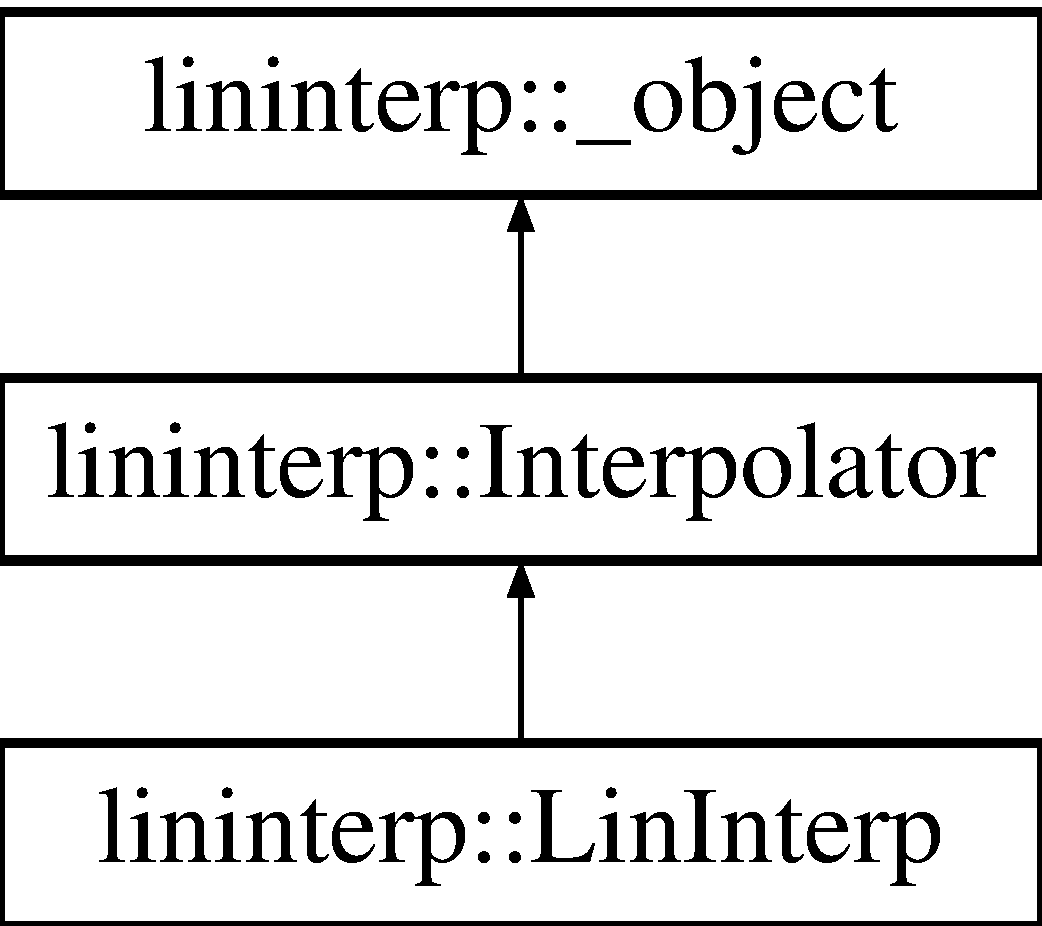
\includegraphics[height=3cm]{d5/dd7/classlininterp_1_1__object}
\end{center}
\end{figure}


The documentation for this class was generated from the following file:\begin{DoxyCompactItemize}
\item 
src/lininterp.py\end{DoxyCompactItemize}

\hypertarget{classmatrix_1_1__object}{
\section{matrix::\_\-object Class Reference}
\label{d8/ddb/classmatrix_1_1__object}\index{matrix::\_\-object@{matrix::\_\-object}}
}
Inheritance diagram for matrix::\_\-object::\begin{figure}[H]
\begin{center}
\leavevmode
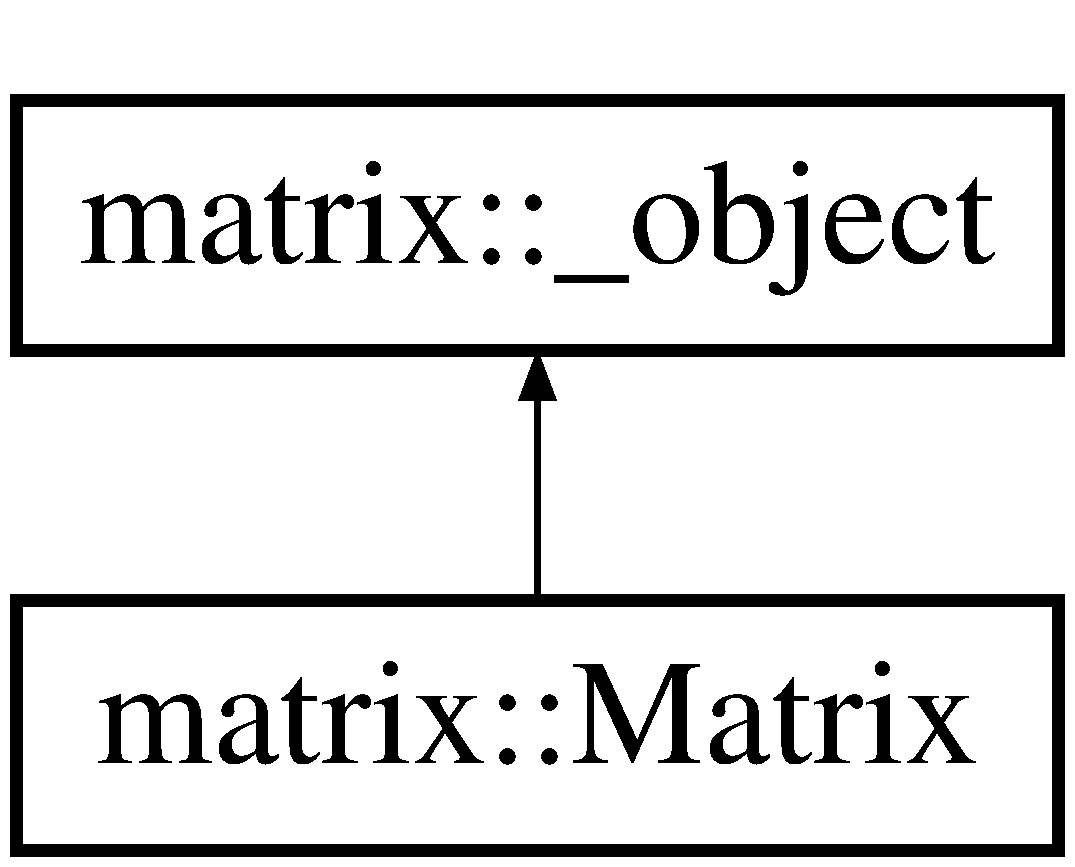
\includegraphics[height=2cm]{d8/ddb/classmatrix_1_1__object}
\end{center}
\end{figure}


The documentation for this class was generated from the following file:\begin{DoxyCompactItemize}
\item 
src/matrix.py\end{DoxyCompactItemize}

\hypertarget{classintegrator_1_1__object}{
\section{integrator::\_\-object Class Reference}
\label{d6/d0c/classintegrator_1_1__object}\index{integrator::\_\-object@{integrator::\_\-object}}
}
Inheritance diagram for integrator::\_\-object::\begin{figure}[H]
\begin{center}
\leavevmode
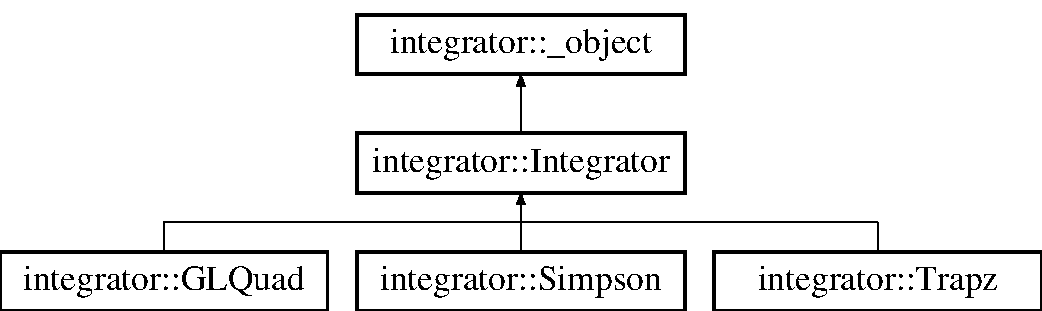
\includegraphics[height=3cm]{d6/d0c/classintegrator_1_1__object}
\end{center}
\end{figure}


The documentation for this class was generated from the following file:\begin{DoxyCompactItemize}
\item 
src/integrator.py\end{DoxyCompactItemize}

\hypertarget{classmatrix3d_1_1__object}{
\section{matrix3d::\_\-object Class Reference}
\label{d7/d99/classmatrix3d_1_1__object}\index{matrix3d::\_\-object@{matrix3d::\_\-object}}
}
Inheritance diagram for matrix3d::\_\-object::\begin{figure}[H]
\begin{center}
\leavevmode
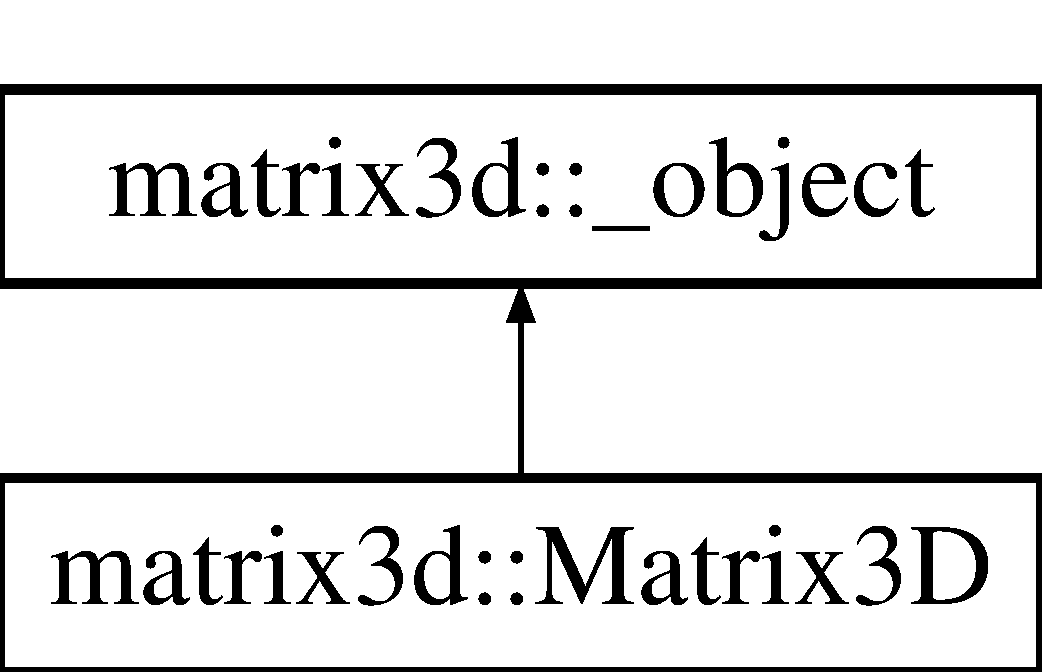
\includegraphics[height=2cm]{d7/d99/classmatrix3d_1_1__object}
\end{center}
\end{figure}


The documentation for this class was generated from the following file:\begin{DoxyCompactItemize}
\item 
src/matrix3d.py\end{DoxyCompactItemize}

\hypertarget{classmatrix4d_1_1__object}{
\section{matrix4d::\_\-object Class Reference}
\label{d5/df5/classmatrix4d_1_1__object}\index{matrix4d::\_\-object@{matrix4d::\_\-object}}
}
Inheritance diagram for matrix4d::\_\-object::\begin{figure}[H]
\begin{center}
\leavevmode
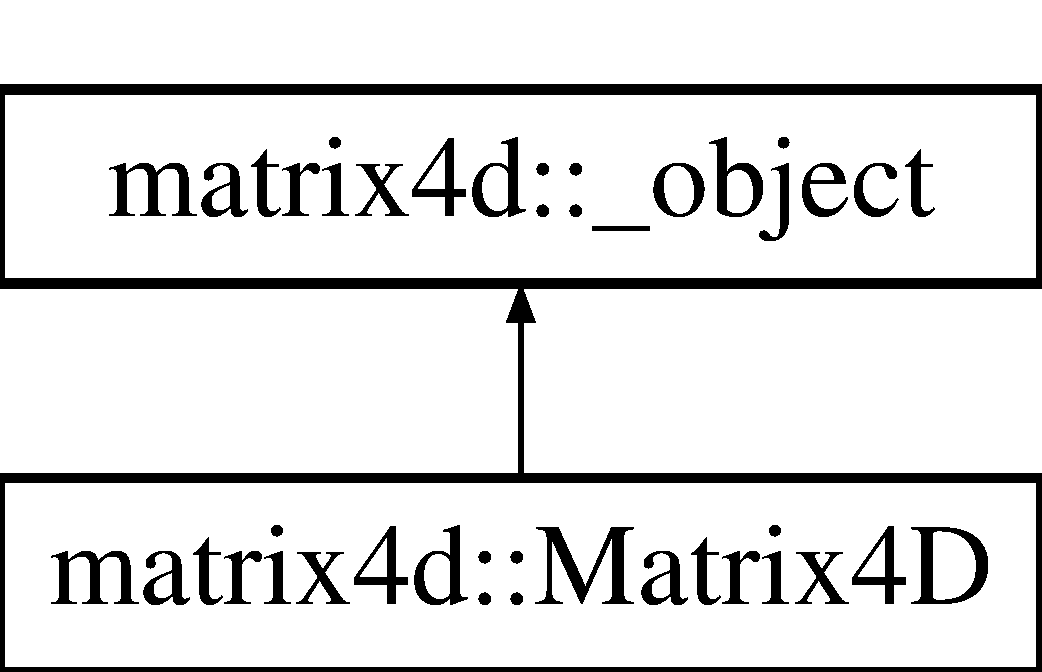
\includegraphics[height=2cm]{d5/df5/classmatrix4d_1_1__object}
\end{center}
\end{figure}


The documentation for this class was generated from the following file:\begin{DoxyCompactItemize}
\item 
src/matrix4d.py\end{DoxyCompactItemize}

\hypertarget{classmaxslope_1_1__object}{
\section{maxslope::\_\-object Class Reference}
\label{d1/d92/classmaxslope_1_1__object}\index{maxslope::\_\-object@{maxslope::\_\-object}}
}
Inheritance diagram for maxslope::\_\-object::\begin{figure}[H]
\begin{center}
\leavevmode
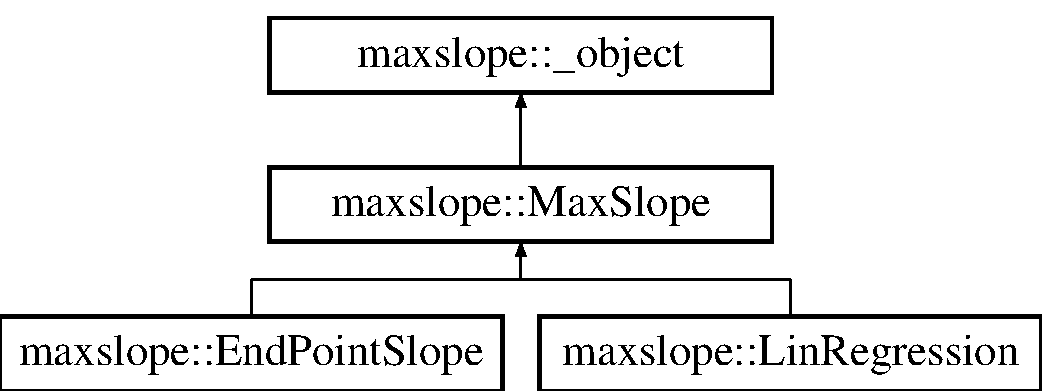
\includegraphics[height=3cm]{d1/d92/classmaxslope_1_1__object}
\end{center}
\end{figure}


The documentation for this class was generated from the following file:\begin{DoxyCompactItemize}
\item 
src/maxslope.py\end{DoxyCompactItemize}

\hypertarget{classleastnonmono_1_1__object}{
\section{leastnonmono::\_\-object Class Reference}
\label{d0/dee/classleastnonmono_1_1__object}\index{leastnonmono::\_\-object@{leastnonmono::\_\-object}}
}
Inheritance diagram for leastnonmono::\_\-object::\begin{figure}[H]
\begin{center}
\leavevmode
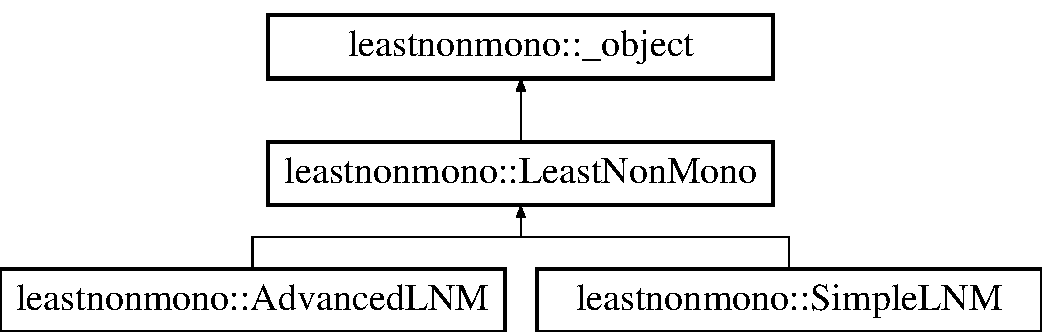
\includegraphics[height=3cm]{d0/dee/classleastnonmono_1_1__object}
\end{center}
\end{figure}


The documentation for this class was generated from the following file:\begin{DoxyCompactItemize}
\item 
src/leastnonmono.py\end{DoxyCompactItemize}

\hypertarget{classmonocheck_1_1__object}{
\section{monocheck::\_\-object Class Reference}
\label{d8/dec/classmonocheck_1_1__object}\index{monocheck::\_\-object@{monocheck::\_\-object}}
}
Inheritance diagram for monocheck::\_\-object::\begin{figure}[H]
\begin{center}
\leavevmode
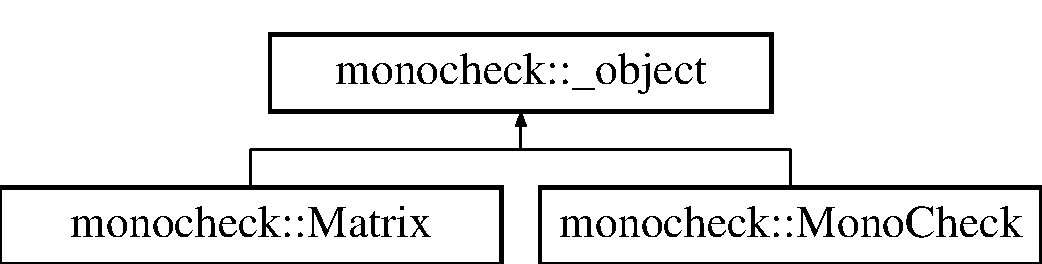
\includegraphics[height=2cm]{d8/dec/classmonocheck_1_1__object}
\end{center}
\end{figure}


The documentation for this class was generated from the following file:\begin{DoxyCompactItemize}
\item 
src/monocheck.py\end{DoxyCompactItemize}

\hypertarget{classpdf_1_1__object}{
\section{pdf::\_\-object Class Reference}
\label{df/d35/classpdf_1_1__object}\index{pdf::\_\-object@{pdf::\_\-object}}
}
Inheritance diagram for pdf::\_\-object::\begin{figure}[H]
\begin{center}
\leavevmode
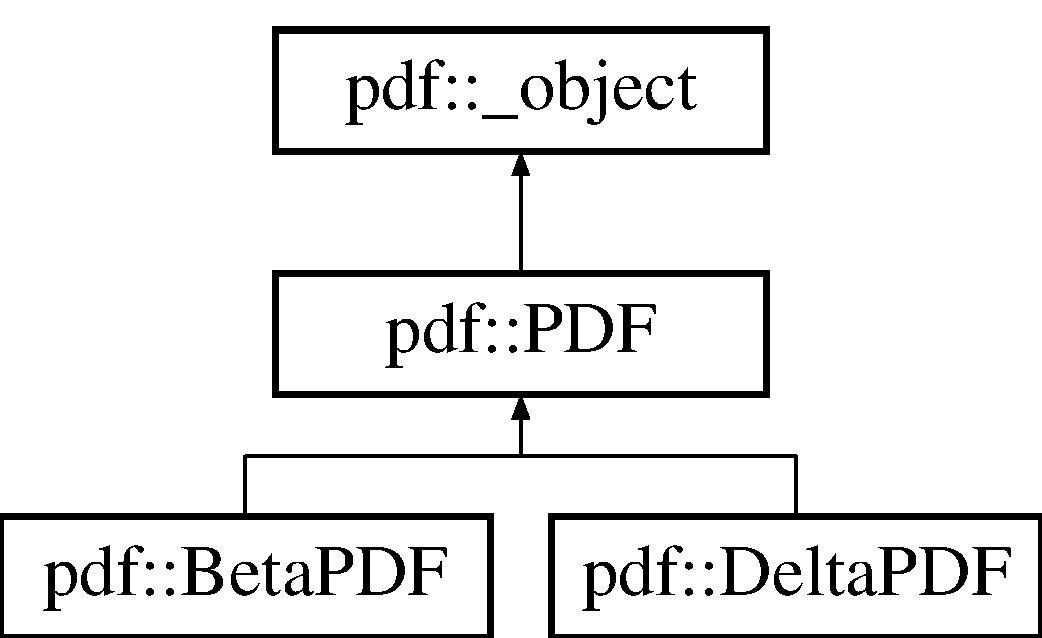
\includegraphics[height=3cm]{df/d35/classpdf_1_1__object}
\end{center}
\end{figure}


The documentation for this class was generated from the following file:\begin{DoxyCompactItemize}
\item 
src/pdf.py\end{DoxyCompactItemize}

\hypertarget{classsorting_1_1__object}{
\section{sorting::\_\-object Class Reference}
\label{da/d16/classsorting_1_1__object}\index{sorting::\_\-object@{sorting::\_\-object}}
}
Inheritance diagram for sorting::\_\-object::\begin{figure}[H]
\begin{center}
\leavevmode
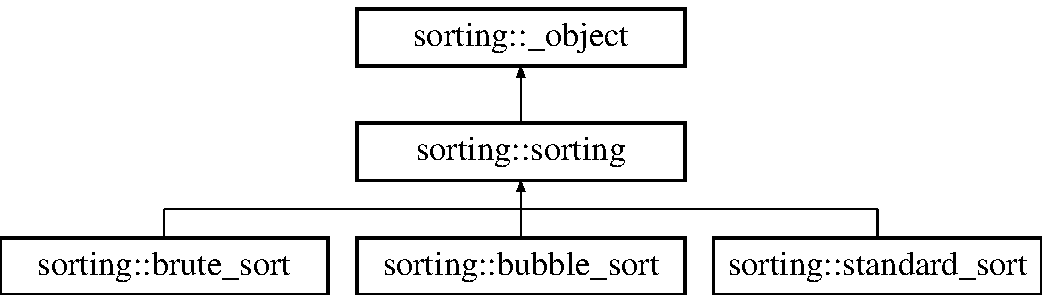
\includegraphics[height=3cm]{da/d16/classsorting_1_1__object}
\end{center}
\end{figure}


The documentation for this class was generated from the following file:\begin{DoxyCompactItemize}
\item 
src/sorting.py\end{DoxyCompactItemize}

\hypertarget{classBetaPDF}{
\section{BetaPDF Class Reference}
\label{de/d4f/classBetaPDF}\index{BetaPDF@{BetaPDF}}
}
Inheritance diagram for BetaPDF::\begin{figure}[H]
\begin{center}
\leavevmode
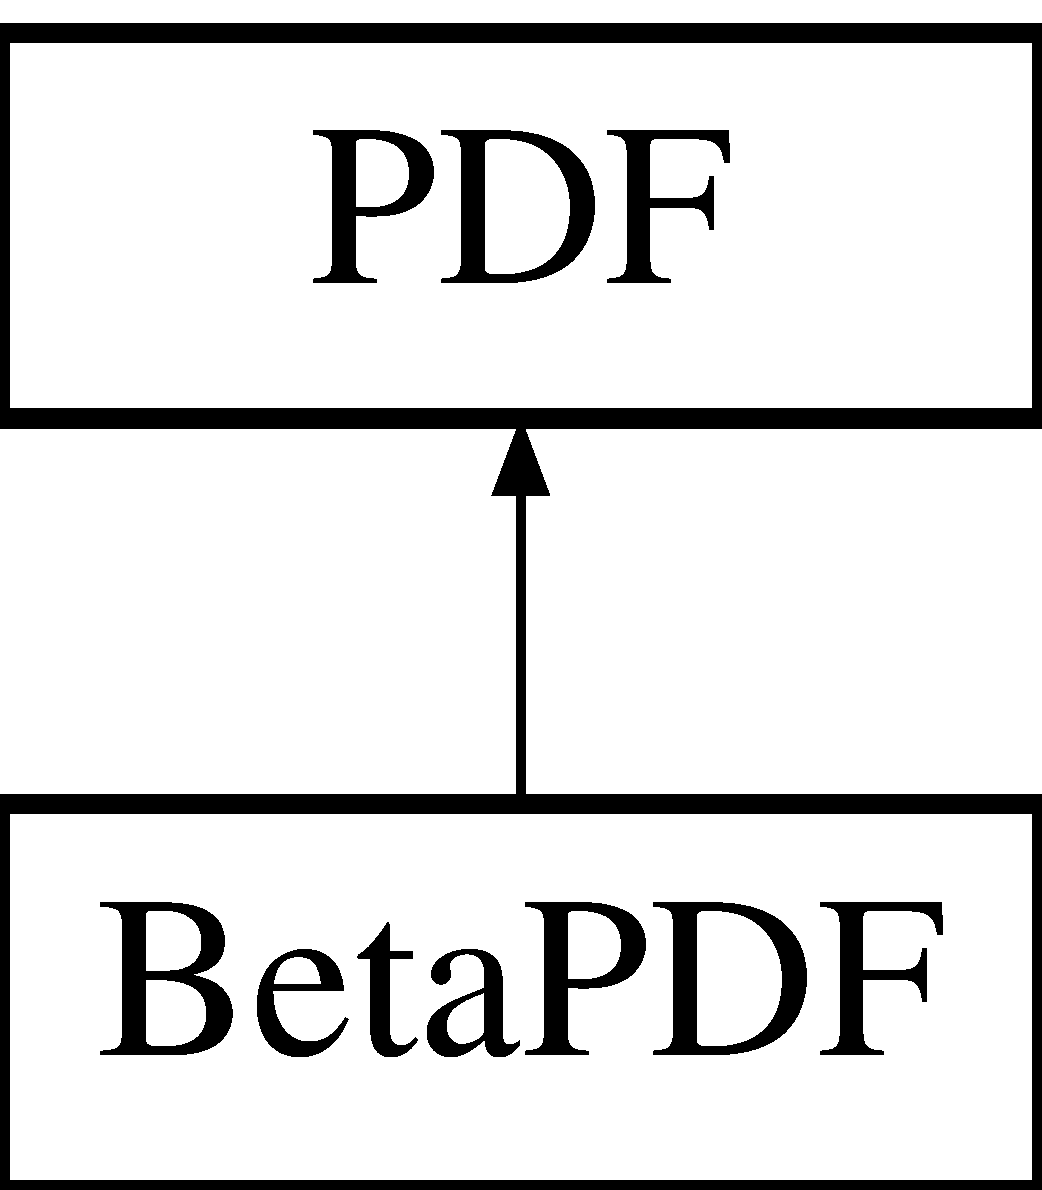
\includegraphics[height=2cm]{de/d4f/classBetaPDF}
\end{center}
\end{figure}
\subsection*{Public Member Functions}
\begin{DoxyCompactItemize}
\item 
\hypertarget{classBetaPDF_a0b5160ebefdcd8b696a45a131bab3261}{
{\bfseries BetaPDF} (const double $\ast$Zmean, const int ZmeanPoints, const double $\ast$Zvar, const int ZvarPoints)}
\label{de/d4f/classBetaPDF_a0b5160ebefdcd8b696a45a131bab3261}

\item 
int \hyperlink{classBetaPDF_a5c27da056f9c9b17af0888fac7df2c9f}{pdfVal} (const double $\ast$Z, const int ZPoints, \hyperlink{classMatrix3D}{Matrix3D} $\ast$pdfValM)
\end{DoxyCompactItemize}


\subsection{Member Function Documentation}
\hypertarget{classBetaPDF_a5c27da056f9c9b17af0888fac7df2c9f}{
\index{BetaPDF@{BetaPDF}!pdfVal@{pdfVal}}
\index{pdfVal@{pdfVal}!BetaPDF@{BetaPDF}}
\subsubsection[{pdfVal}]{\setlength{\rightskip}{0pt plus 5cm}int BetaPDF::pdfVal (const double $\ast$ {\em Z}, \/  const int {\em ZPoints}, \/  {\bf Matrix3D} $\ast$ {\em pdfValM})\hspace{0.3cm}{\ttfamily  \mbox{[}virtual\mbox{]}}}}
\label{de/d4f/classBetaPDF_a5c27da056f9c9b17af0888fac7df2c9f}


check for Min or Max mean

Delta \hyperlink{classPDF}{PDF} for zero variance

Impossible cases: becomes double delta \hyperlink{classPDF}{PDF}

\hyperlink{classBetaPDF}{BetaPDF}

Middle points: 0 $<$ n $<$ ZPoints-\/1

Calculate integral at ends

Set \hyperlink{classPDF}{PDF} to output 

Implements \hyperlink{classPDF}{PDF}.

The documentation for this class was generated from the following files:\begin{DoxyCompactItemize}
\item 
src/betaPDF.h\item 
src/betaPDF.cc\end{DoxyCompactItemize}

\hypertarget{classpdf_1_1BetaPDF}{
\section{pdf::BetaPDF Class Reference}
\label{d4/dae/classpdf_1_1BetaPDF}\index{pdf::BetaPDF@{pdf::BetaPDF}}
}
Inheritance diagram for pdf::BetaPDF::\begin{figure}[H]
\begin{center}
\leavevmode
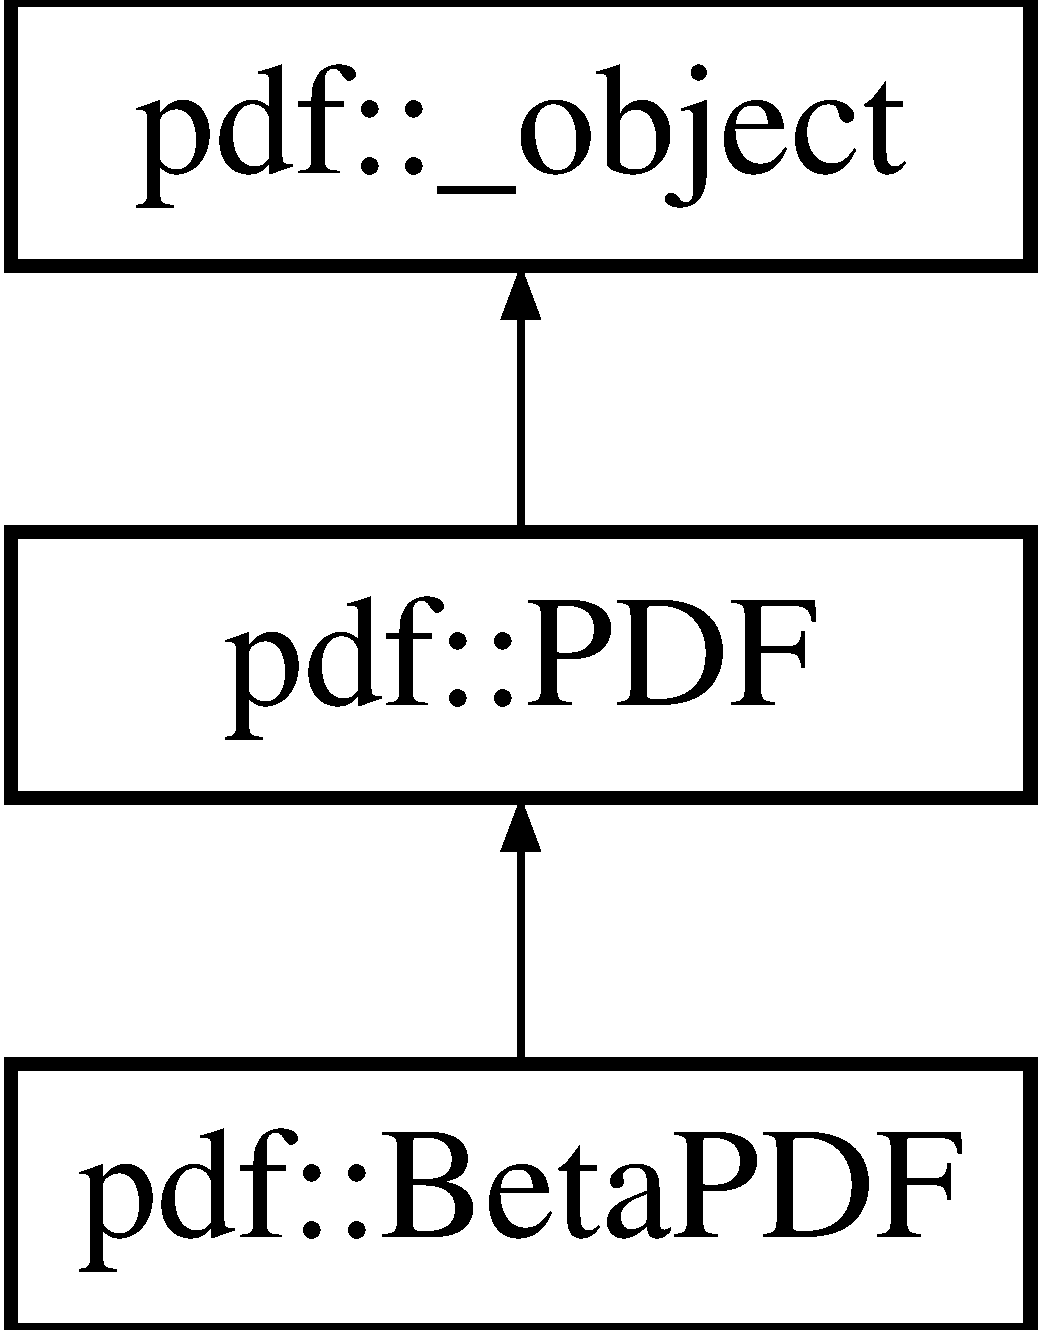
\includegraphics[height=3cm]{d4/dae/classpdf_1_1BetaPDF}
\end{center}
\end{figure}
\subsection*{Public Member Functions}
\begin{DoxyCompactItemize}
\item 
\hypertarget{classpdf_1_1BetaPDF_a20df6a985b59544305063ed17b7358c5}{
def {\bfseries \_\-\_\-init\_\-\_\-}}
\label{d4/dae/classpdf_1_1BetaPDF_a20df6a985b59544305063ed17b7358c5}

\item 
\hypertarget{classpdf_1_1BetaPDF_ad7f9b56263693e180c38d788048299f0}{
def {\bfseries pdfVal}}
\label{d4/dae/classpdf_1_1BetaPDF_ad7f9b56263693e180c38d788048299f0}

\end{DoxyCompactItemize}
\subsection*{Public Attributes}
\begin{DoxyCompactItemize}
\item 
\hypertarget{classpdf_1_1BetaPDF_afec5aec12f1405624850046968b2bbec}{
{\bfseries this}}
\label{d4/dae/classpdf_1_1BetaPDF_afec5aec12f1405624850046968b2bbec}

\end{DoxyCompactItemize}


The documentation for this class was generated from the following file:\begin{DoxyCompactItemize}
\item 
src/pdf.py\end{DoxyCompactItemize}

\hypertarget{classsorting_1_1brute__sort}{
\section{sorting::brute\_\-sort Class Reference}
\label{d0/da8/classsorting_1_1brute__sort}\index{sorting::brute\_\-sort@{sorting::brute\_\-sort}}
}
Inheritance diagram for sorting::brute\_\-sort::\begin{figure}[H]
\begin{center}
\leavevmode
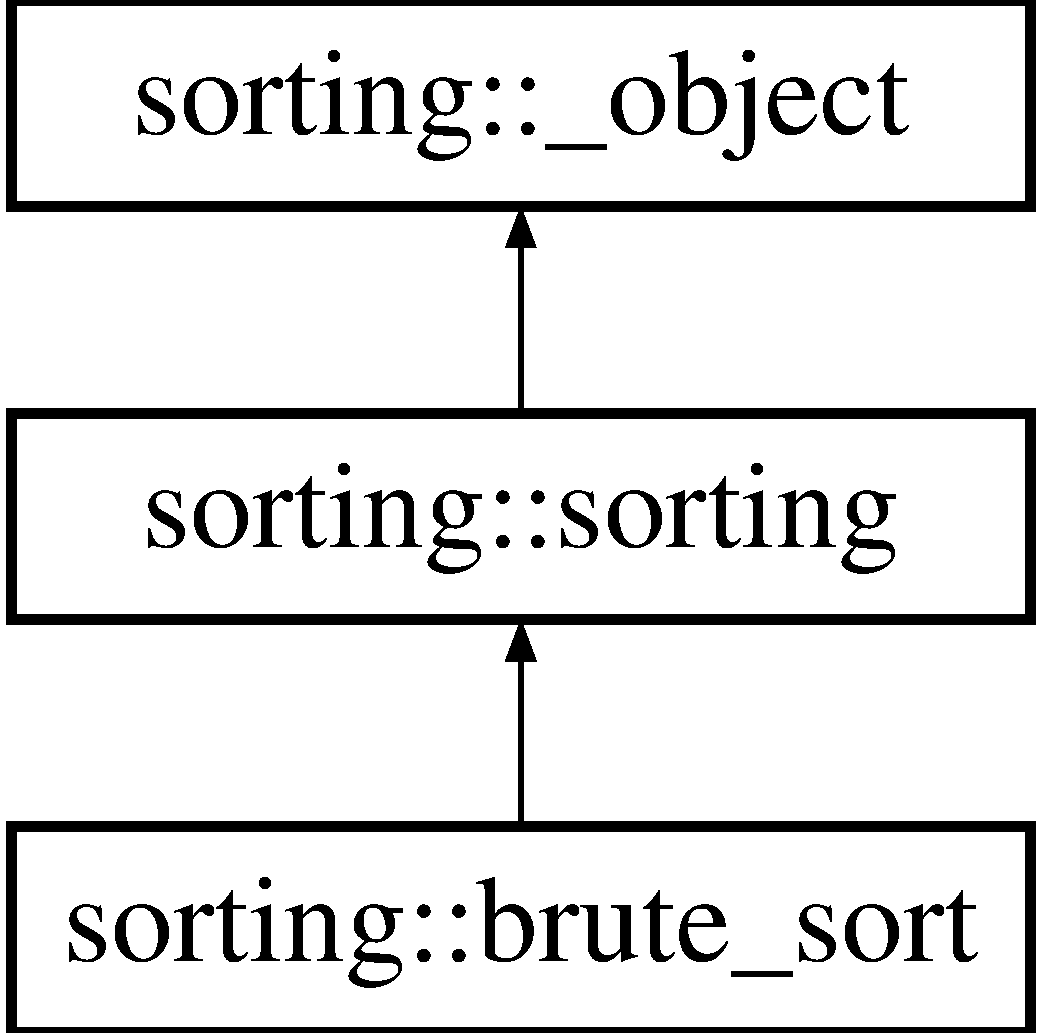
\includegraphics[height=3cm]{d0/da8/classsorting_1_1brute__sort}
\end{center}
\end{figure}
\subsection*{Public Member Functions}
\begin{DoxyCompactItemize}
\item 
\hypertarget{classsorting_1_1brute__sort_aa845948c1030d3cd0922c3322f16f789}{
def {\bfseries \_\-\_\-init\_\-\_\-}}
\label{d0/da8/classsorting_1_1brute__sort_aa845948c1030d3cd0922c3322f16f789}

\item 
\hypertarget{classsorting_1_1brute__sort_a0d206532a6c29ac13e0f76b1b6cfc9ca}{
def {\bfseries sort\_\-data}}
\label{d0/da8/classsorting_1_1brute__sort_a0d206532a6c29ac13e0f76b1b6cfc9ca}

\item 
\hypertarget{classsorting_1_1brute__sort_a07dc13d397462f069f699a721198ce41}{
def {\bfseries SetRefColNum}}
\label{d0/da8/classsorting_1_1brute__sort_a07dc13d397462f069f699a721198ce41}

\item 
\hypertarget{classsorting_1_1brute__sort_a5969ba91785fa7e8185c0a42ecd5b6f5}{
def {\bfseries extractRefCol}}
\label{d0/da8/classsorting_1_1brute__sort_a5969ba91785fa7e8185c0a42ecd5b6f5}

\item 
\hypertarget{classsorting_1_1brute__sort_a7e948e1976abc0cac6913f8fd89c62c7}{
def {\bfseries generateIndexArray}}
\label{d0/da8/classsorting_1_1brute__sort_a7e948e1976abc0cac6913f8fd89c62c7}

\item 
\hypertarget{classsorting_1_1brute__sort_a99e2001754a0dab53f293119f59f4c27}{
def {\bfseries SetSortStartIndex}}
\label{d0/da8/classsorting_1_1brute__sort_a99e2001754a0dab53f293119f59f4c27}

\item 
\hypertarget{classsorting_1_1brute__sort_a584b9ceb12f2bfa3f370e8269a7e028e}{
def {\bfseries SetSortEndIndex}}
\label{d0/da8/classsorting_1_1brute__sort_a584b9ceb12f2bfa3f370e8269a7e028e}

\end{DoxyCompactItemize}
\subsection*{Public Attributes}
\begin{DoxyCompactItemize}
\item 
\hypertarget{classsorting_1_1brute__sort_a44f3eb7349db40f6b417ab5fecb36927}{
{\bfseries this}}
\label{d0/da8/classsorting_1_1brute__sort_a44f3eb7349db40f6b417ab5fecb36927}

\end{DoxyCompactItemize}


The documentation for this class was generated from the following file:\begin{DoxyCompactItemize}
\item 
src/sorting.py\end{DoxyCompactItemize}

\hypertarget{classbrute__sort}{
\section{brute\_\-sort Class Reference}
\label{d3/d39/classbrute__sort}\index{brute\_\-sort@{brute\_\-sort}}
}
Inheritance diagram for brute\_\-sort::\begin{figure}[H]
\begin{center}
\leavevmode
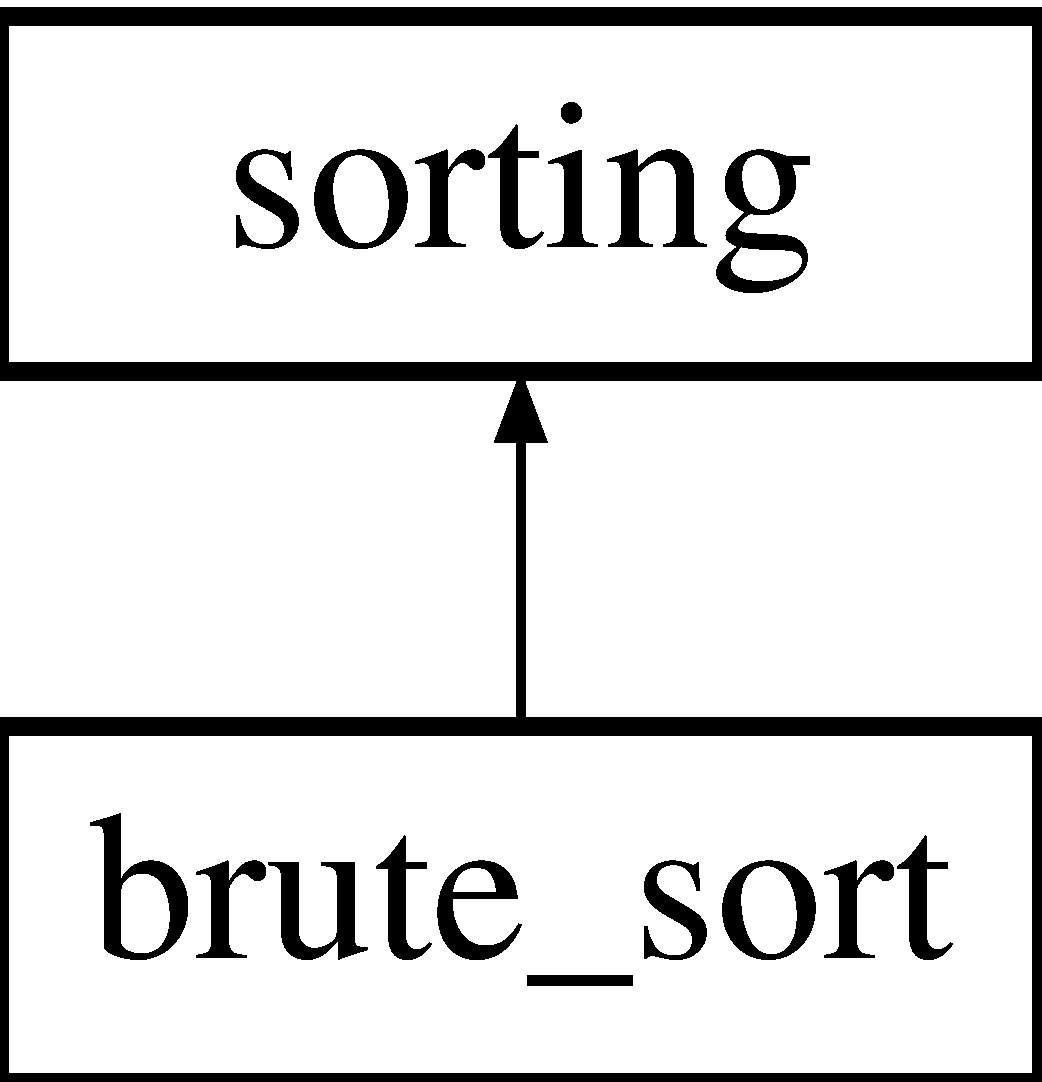
\includegraphics[height=2cm]{d3/d39/classbrute__sort}
\end{center}
\end{figure}
\subsection*{Public Member Functions}
\begin{DoxyCompactItemize}
\item 
\hyperlink{classbrute__sort_a2dbbb3b1c89d6a5720d79a5bf150ad1f}{brute\_\-sort} (\hyperlink{classMatrix}{Matrix} $\ast$data)
\begin{DoxyCompactList}\small\item\em Constructor. \item\end{DoxyCompactList}\item 
\hypertarget{classbrute__sort_a0c5f47456d59d36d8b2370196d953b81}{
\hyperlink{classbrute__sort_a0c5f47456d59d36d8b2370196d953b81}{$\sim$brute\_\-sort} ()}
\label{d3/d39/classbrute__sort_a0c5f47456d59d36d8b2370196d953b81}

\begin{DoxyCompactList}\small\item\em Destructor. \item\end{DoxyCompactList}\item 
int \hyperlink{classbrute__sort_a377b8811e92553a66cdb6780c43e16e6}{sort\_\-data} ()
\begin{DoxyCompactList}\small\item\em Main function that sorts the given data. \item\end{DoxyCompactList}\item 
\hypertarget{classbrute__sort_a7d43275af73d67695f2736dcada07b86}{
void \hyperlink{classbrute__sort_a7d43275af73d67695f2736dcada07b86}{SetRefColNum} (int num)}
\label{d3/d39/classbrute__sort_a7d43275af73d67695f2736dcada07b86}

\begin{DoxyCompactList}\small\item\em Set the reference column number. \item\end{DoxyCompactList}\end{DoxyCompactItemize}


\subsection{Constructor \& Destructor Documentation}
\hypertarget{classbrute__sort_a2dbbb3b1c89d6a5720d79a5bf150ad1f}{
\index{brute\_\-sort@{brute\_\-sort}!brute\_\-sort@{brute\_\-sort}}
\index{brute\_\-sort@{brute\_\-sort}!brute_sort@{brute\_\-sort}}
\subsubsection[{brute\_\-sort}]{\setlength{\rightskip}{0pt plus 5cm}{\bf brute\_\-sort::brute\_\-sort} ({\bf Matrix} $\ast$ {\em data})}}
\label{d3/d39/classbrute__sort_a2dbbb3b1c89d6a5720d79a5bf150ad1f}


Constructor. This algorithm goes over the each entry (rows times) at the selected column, finds the maximum entry, records its index. This is repeated rows times until the indices of the entries are obtained in order. Then each column of the matrix is reordered using these indices. 

\subsection{Member Function Documentation}
\hypertarget{classbrute__sort_a377b8811e92553a66cdb6780c43e16e6}{
\index{brute\_\-sort@{brute\_\-sort}!sort\_\-data@{sort\_\-data}}
\index{sort\_\-data@{sort\_\-data}!brute_sort@{brute\_\-sort}}
\subsubsection[{sort\_\-data}]{\setlength{\rightskip}{0pt plus 5cm}int brute\_\-sort::sort\_\-data ()\hspace{0.3cm}{\ttfamily  \mbox{[}virtual\mbox{]}}}}
\label{d3/d39/classbrute__sort_a377b8811e92553a66cdb6780c43e16e6}


Main function that sorts the given data. The algortihm processes the reference column and sorts it using the brute sort approach.

\begin{DoxyVerb}
  INPUT:

  There are no inputs. The data to be sorted is already passed via the constructor

  
  OUTPUT:

  int          flag specifying whether or not the function succeeded
                = 0: success
	       != 0: something went wrong

  \end{DoxyVerb}
 

Implements \hyperlink{classsorting_a94c4b729732743299f3dcd2505312381}{sorting}.

The documentation for this class was generated from the following files:\begin{DoxyCompactItemize}
\item 
src/brute\_\-sort.h\item 
src/brute\_\-sort.cc\end{DoxyCompactItemize}

\hypertarget{classsorting_1_1bubble__sort}{
\section{sorting::bubble\_\-sort Class Reference}
\label{dc/ddd/classsorting_1_1bubble__sort}\index{sorting::bubble\_\-sort@{sorting::bubble\_\-sort}}
}
Inheritance diagram for sorting::bubble\_\-sort::\begin{figure}[H]
\begin{center}
\leavevmode
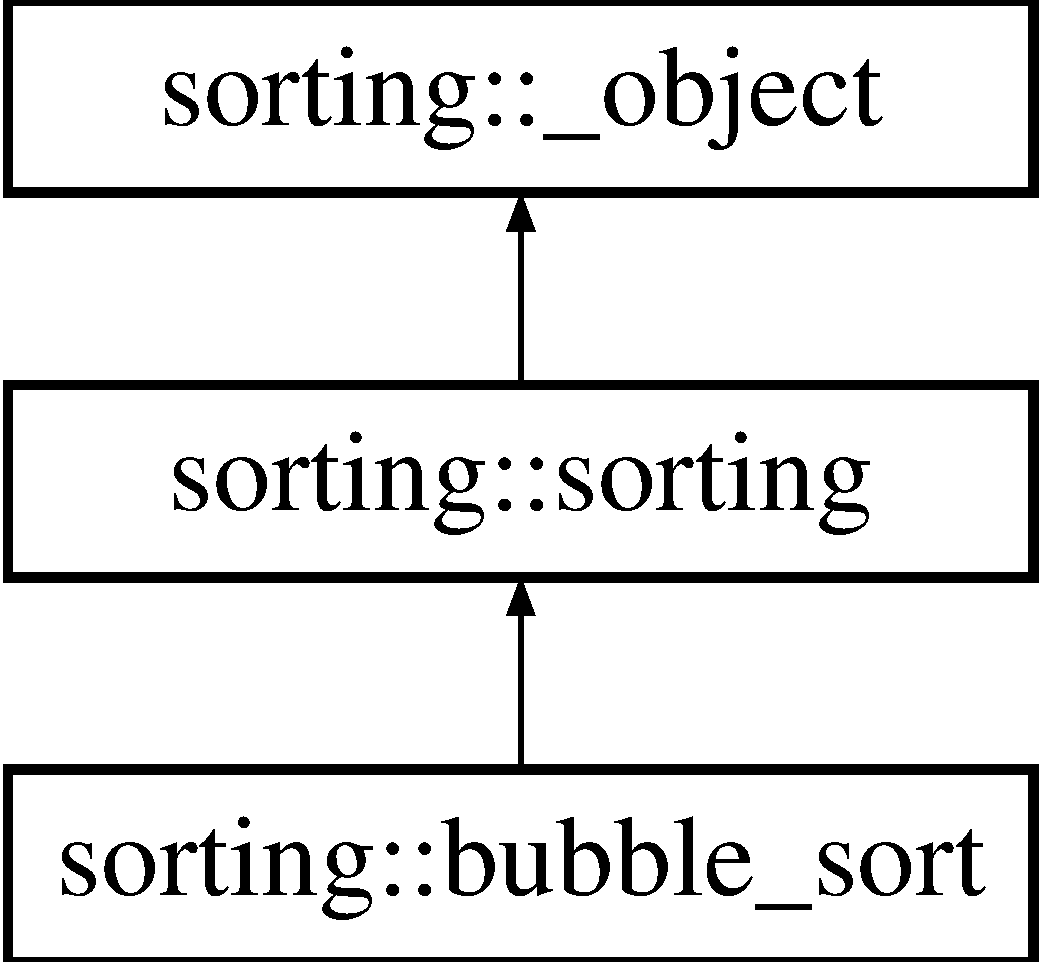
\includegraphics[height=3cm]{dc/ddd/classsorting_1_1bubble__sort}
\end{center}
\end{figure}
\subsection*{Public Member Functions}
\begin{DoxyCompactItemize}
\item 
\hypertarget{classsorting_1_1bubble__sort_a41429408d3f230ce2b68acaeacabe719}{
def {\bfseries \_\-\_\-init\_\-\_\-}}
\label{dc/ddd/classsorting_1_1bubble__sort_a41429408d3f230ce2b68acaeacabe719}

\item 
\hypertarget{classsorting_1_1bubble__sort_a25f3566a6fe7dac1291ae1ca3b190f6d}{
def {\bfseries sort\_\-data}}
\label{dc/ddd/classsorting_1_1bubble__sort_a25f3566a6fe7dac1291ae1ca3b190f6d}

\item 
\hypertarget{classsorting_1_1bubble__sort_aa4d91cd959905d26975604a165687d6e}{
def {\bfseries SetRefColNum}}
\label{dc/ddd/classsorting_1_1bubble__sort_aa4d91cd959905d26975604a165687d6e}

\item 
\hypertarget{classsorting_1_1bubble__sort_a10ece0df6466a21213006beea777f3d9}{
def {\bfseries extractRefCol}}
\label{dc/ddd/classsorting_1_1bubble__sort_a10ece0df6466a21213006beea777f3d9}

\item 
\hypertarget{classsorting_1_1bubble__sort_aa5818ee4017096a296d6943054f4831a}{
def {\bfseries generateIndexArray}}
\label{dc/ddd/classsorting_1_1bubble__sort_aa5818ee4017096a296d6943054f4831a}

\item 
\hypertarget{classsorting_1_1bubble__sort_afbc885145ee1afd6eec22814143ea480}{
def {\bfseries SetSortStartIndex}}
\label{dc/ddd/classsorting_1_1bubble__sort_afbc885145ee1afd6eec22814143ea480}

\item 
\hypertarget{classsorting_1_1bubble__sort_aa1c565331e9ca1c884fd86b7e94ca253}{
def {\bfseries SetSortEndIndex}}
\label{dc/ddd/classsorting_1_1bubble__sort_aa1c565331e9ca1c884fd86b7e94ca253}

\end{DoxyCompactItemize}
\subsection*{Public Attributes}
\begin{DoxyCompactItemize}
\item 
\hypertarget{classsorting_1_1bubble__sort_ad9ac15e871f8737d8513e7ee1097c5e4}{
{\bfseries this}}
\label{dc/ddd/classsorting_1_1bubble__sort_ad9ac15e871f8737d8513e7ee1097c5e4}

\end{DoxyCompactItemize}


The documentation for this class was generated from the following file:\begin{DoxyCompactItemize}
\item 
src/sorting.py\end{DoxyCompactItemize}

\hypertarget{classbubble__sort}{
\section{bubble\_\-sort Class Reference}
\label{dc/d2f/classbubble__sort}\index{bubble\_\-sort@{bubble\_\-sort}}
}
Inheritance diagram for bubble\_\-sort::\begin{figure}[H]
\begin{center}
\leavevmode
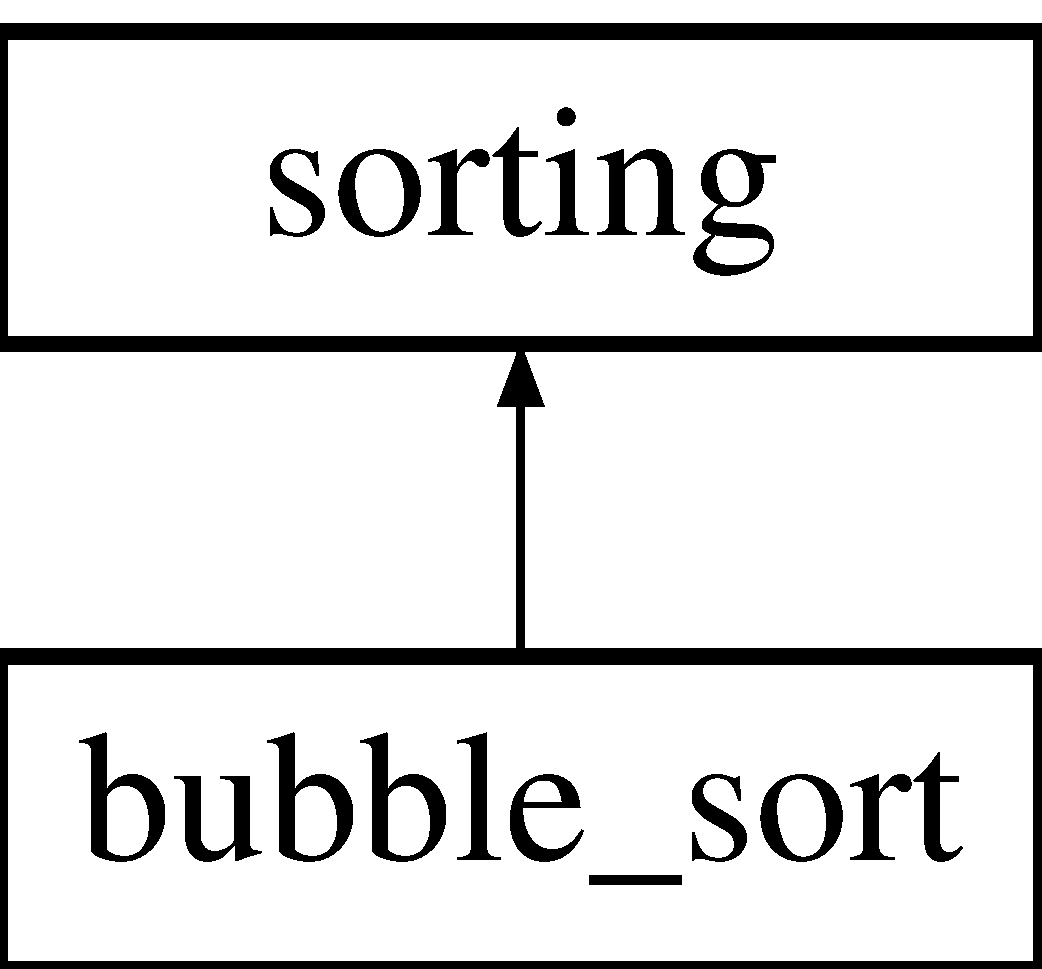
\includegraphics[height=2cm]{dc/d2f/classbubble__sort}
\end{center}
\end{figure}
\subsection*{Public Member Functions}
\begin{DoxyCompactItemize}
\item 
\hyperlink{classbubble__sort_aa413fc87fd7b9a0da354c0da0bfc0fa2}{bubble\_\-sort} (\hyperlink{classMatrix}{Matrix} $\ast$data)
\item 
\hypertarget{classbubble__sort_ad33134a9337963c4a3e39397bdd5d09d}{
\hyperlink{classbubble__sort_ad33134a9337963c4a3e39397bdd5d09d}{$\sim$bubble\_\-sort} ()}
\label{dc/d2f/classbubble__sort_ad33134a9337963c4a3e39397bdd5d09d}

\begin{DoxyCompactList}\small\item\em Destructor. \item\end{DoxyCompactList}\item 
int \hyperlink{classbubble__sort_a8fdc845adc8e24bbb169b79ef5140ee2}{sort\_\-data} ()
\begin{DoxyCompactList}\small\item\em Main \hyperlink{classsorting}{sorting} body. \item\end{DoxyCompactList}\item 
\hypertarget{classbubble__sort_af950c87cd047c9d26b12cba8e06e6326}{
void \hyperlink{classbubble__sort_af950c87cd047c9d26b12cba8e06e6326}{SetRefColNum} (int num)}
\label{dc/d2f/classbubble__sort_af950c87cd047c9d26b12cba8e06e6326}

\begin{DoxyCompactList}\small\item\em Set the reference column number and extract the data of the reference column to the container refColumn\_\-. \item\end{DoxyCompactList}\end{DoxyCompactItemize}


\subsection{Constructor \& Destructor Documentation}
\hypertarget{classbubble__sort_aa413fc87fd7b9a0da354c0da0bfc0fa2}{
\index{bubble\_\-sort@{bubble\_\-sort}!bubble\_\-sort@{bubble\_\-sort}}
\index{bubble\_\-sort@{bubble\_\-sort}!bubble_sort@{bubble\_\-sort}}
\subsubsection[{bubble\_\-sort}]{\setlength{\rightskip}{0pt plus 5cm}bubble\_\-sort::bubble\_\-sort ({\bf Matrix} $\ast$ {\em data})}}
\label{dc/d2f/classbubble__sort_aa413fc87fd7b9a0da354c0da0bfc0fa2}
The constructor duplicates the data from the matrix pointer to datacopy\_\- object. It also generates the array containing the indices to be used during \hyperlink{classsorting}{sorting}. 

\subsection{Member Function Documentation}
\hypertarget{classbubble__sort_a8fdc845adc8e24bbb169b79ef5140ee2}{
\index{bubble\_\-sort@{bubble\_\-sort}!sort\_\-data@{sort\_\-data}}
\index{sort\_\-data@{sort\_\-data}!bubble_sort@{bubble\_\-sort}}
\subsubsection[{sort\_\-data}]{\setlength{\rightskip}{0pt plus 5cm}int bubble\_\-sort::sort\_\-data ()\hspace{0.3cm}{\ttfamily  \mbox{[}virtual\mbox{]}}}}
\label{dc/d2f/classbubble__sort_a8fdc845adc8e24bbb169b79ef5140ee2}


Main \hyperlink{classsorting}{sorting} body. Details of the bubble sort algortihm can be found from the following link: \href{http://en.wikipedia.org/wiki/Bubble_sort}{\tt http://en.wikipedia.org/wiki/Bubble\_\-sort} 

Implements \hyperlink{classsorting_a94c4b729732743299f3dcd2505312381}{sorting}.

The documentation for this class was generated from the following files:\begin{DoxyCompactItemize}
\item 
src/bubble\_\-sort.h\item 
src/bubble\_\-sort.cc\end{DoxyCompactItemize}

\hypertarget{classCompVec}{
\section{CompVec Class Reference}
\label{d7/d1f/classCompVec}\index{CompVec@{CompVec}}
}


Comparator for the standard sorting algorithm.  
\subsection*{Public Member Functions}
\begin{DoxyCompactItemize}
\item 
\hypertarget{classCompVec_a6963b86bb7b027c564f9fcbfa48631ff}{
{\bfseries CompVec} (double $\ast$arr)}
\label{d7/d1f/classCompVec_a6963b86bb7b027c564f9fcbfa48631ff}

\item 
\hypertarget{classCompVec_af72aba58e4ec029df30580c71c965490}{
bool {\bfseries operator()} (size\_\-t i, size\_\-t j)}
\label{d7/d1f/classCompVec_af72aba58e4ec029df30580c71c965490}

\end{DoxyCompactItemize}


\subsection{Detailed Description}
Comparator for the standard sorting algorithm. 

The documentation for this class was generated from the following file:\begin{DoxyCompactItemize}
\item 
src/standardsort.cc\end{DoxyCompactItemize}

\hypertarget{classDeltaPDF}{
\section{DeltaPDF Class Reference}
\label{dd/d98/classDeltaPDF}\index{DeltaPDF@{DeltaPDF}}
}


Evaluates delta \hyperlink{classPDF}{PDF} and stores values in a \hyperlink{classMatrix3D}{Matrix3D} object.  


{\ttfamily \#include $<$deltaPDF.h$>$}Inheritance diagram for DeltaPDF::\begin{figure}[H]
\begin{center}
\leavevmode
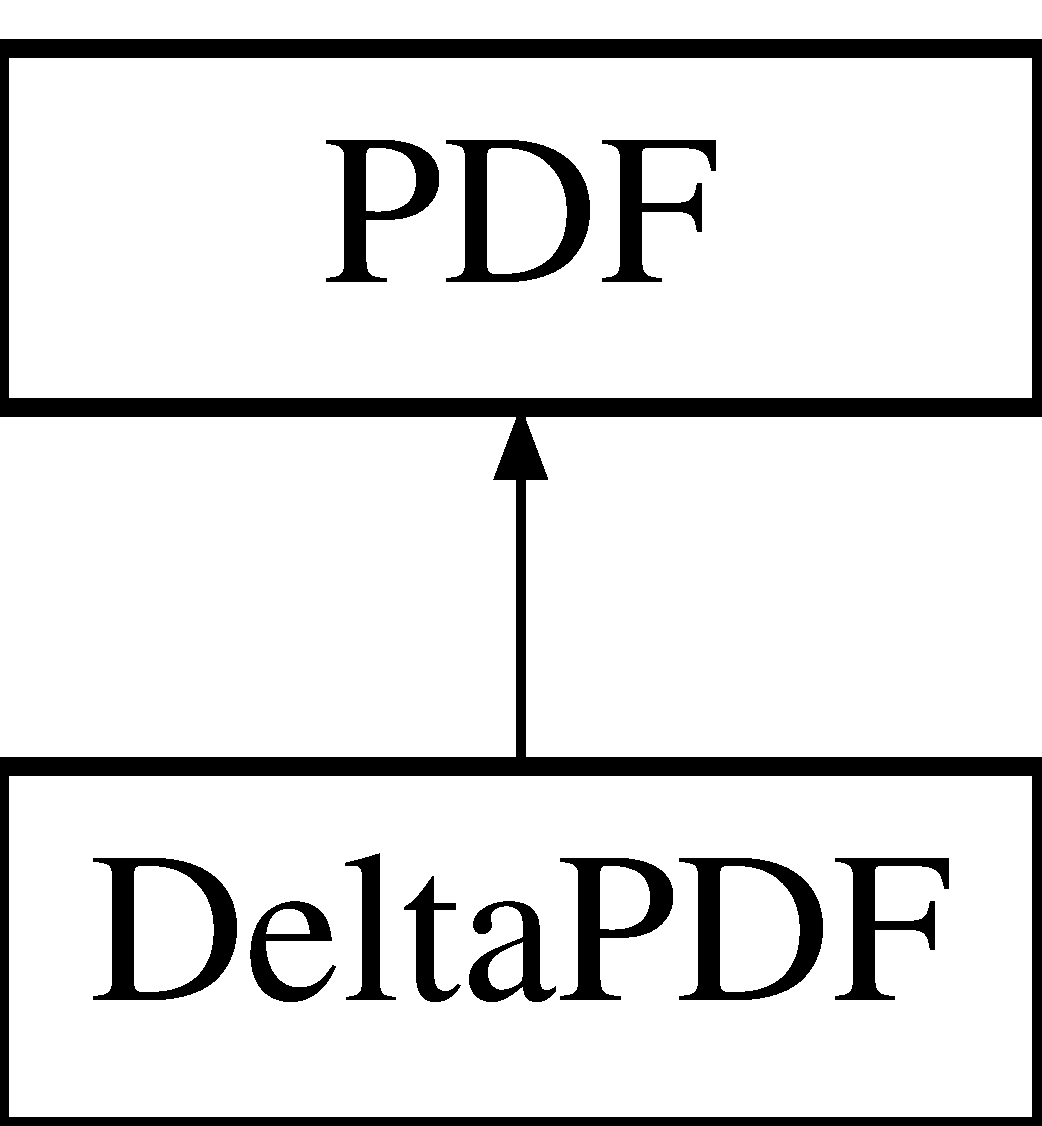
\includegraphics[height=2cm]{dd/d98/classDeltaPDF}
\end{center}
\end{figure}
\subsection*{Public Member Functions}
\begin{DoxyCompactItemize}
\item 
\hypertarget{classDeltaPDF_a6268a222dac459788d7a7589e0bec1c5}{
\hyperlink{classDeltaPDF_a6268a222dac459788d7a7589e0bec1c5}{DeltaPDF} (const double $\ast$Zmean, const int ZmeanPoints)}
\label{dd/d98/classDeltaPDF_a6268a222dac459788d7a7589e0bec1c5}

\begin{DoxyCompactList}\small\item\em Constructor. \item\end{DoxyCompactList}\item 
\hypertarget{classDeltaPDF_a9539ed9f2f24966af76b6bba4734b2be}{
\hyperlink{classDeltaPDF_a9539ed9f2f24966af76b6bba4734b2be}{$\sim$DeltaPDF} ()}
\label{dd/d98/classDeltaPDF_a9539ed9f2f24966af76b6bba4734b2be}

\begin{DoxyCompactList}\small\item\em Destructor. \item\end{DoxyCompactList}\item 
int \hyperlink{classDeltaPDF_a787e205c3bd8d4f95f7c528497e3a617}{pdfVal} (const double $\ast$Z, const int ZPoints, \hyperlink{classMatrix3D}{Matrix3D} $\ast$pdfValM)
\end{DoxyCompactItemize}


\subsection{Detailed Description}
Evaluates delta \hyperlink{classPDF}{PDF} and stores values in a \hyperlink{classMatrix3D}{Matrix3D} object. 

\subsection{Member Function Documentation}
\hypertarget{classDeltaPDF_a787e205c3bd8d4f95f7c528497e3a617}{
\index{DeltaPDF@{DeltaPDF}!pdfVal@{pdfVal}}
\index{pdfVal@{pdfVal}!DeltaPDF@{DeltaPDF}}
\subsubsection[{pdfVal}]{\setlength{\rightskip}{0pt plus 5cm}int DeltaPDF::pdfVal (const double $\ast$ {\em Z}, \/  const int {\em ZPoints}, \/  {\bf Matrix3D} $\ast$ {\em pdfValM})\hspace{0.3cm}{\ttfamily  \mbox{[}virtual\mbox{]}}}}
\label{dd/d98/classDeltaPDF_a787e205c3bd8d4f95f7c528497e3a617}
The Delta \hyperlink{classPDF}{PDF} uses statistics (means) to generate a \hyperlink{classPDF}{PDF}. The \hyperlink{classPDF}{PDF} values are stored in a \hyperlink{classMatrix3D}{Matrix3D} object: dim1 is the variance, dim2 is the mean, and dim3 are the data points.

\begin{DoxyVerb}
  
  INPUTS: 
  
  const double *Z           double arrray containing mixture fraction values coming from the files

  const int ZPoints         number of mixture fraction values in the Z array

  Matrix3D* pdfValm         the Matrix3D type container that stores the PDF values


  OUTPUT:

  int                       flag specifying whether or not the function succeeded
                             = 0: success
			    != 0: something went wrong

  \end{DoxyVerb}
 

Implements \hyperlink{classPDF}{PDF}.

The documentation for this class was generated from the following files:\begin{DoxyCompactItemize}
\item 
src/deltaPDF.h\item 
src/deltaPDF.cc\end{DoxyCompactItemize}

\hypertarget{classpdf_1_1DeltaPDF}{
\section{pdf::DeltaPDF Class Reference}
\label{dc/d18/classpdf_1_1DeltaPDF}\index{pdf::DeltaPDF@{pdf::DeltaPDF}}
}
Inheritance diagram for pdf::DeltaPDF::\begin{figure}[H]
\begin{center}
\leavevmode
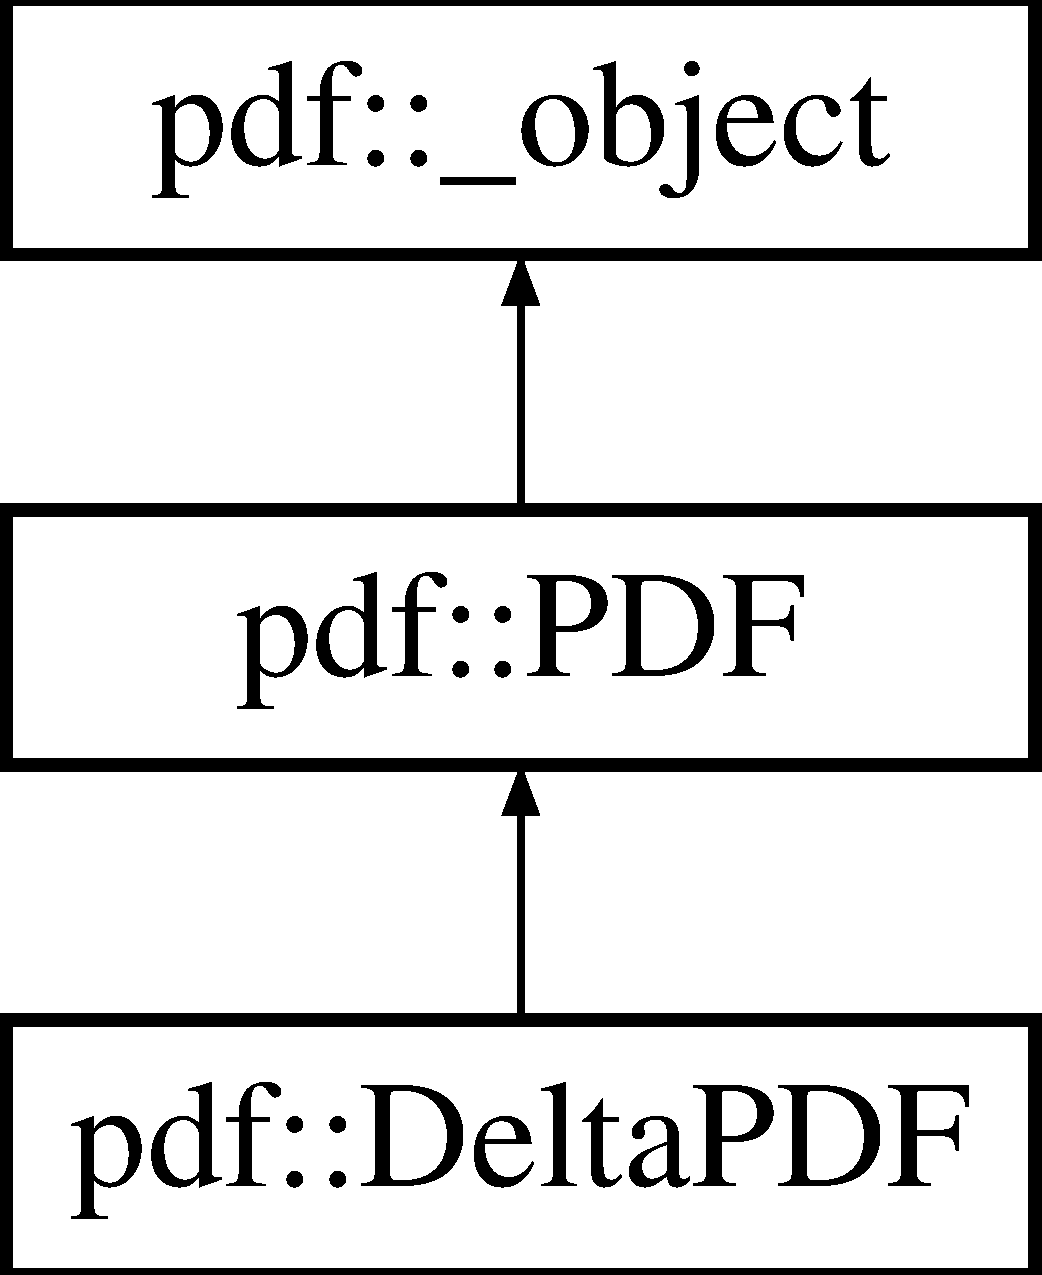
\includegraphics[height=3cm]{dc/d18/classpdf_1_1DeltaPDF}
\end{center}
\end{figure}
\subsection*{Public Member Functions}
\begin{DoxyCompactItemize}
\item 
\hypertarget{classpdf_1_1DeltaPDF_a6fdc3ea1145460c7872f078ae4c53f47}{
def {\bfseries \_\-\_\-init\_\-\_\-}}
\label{dc/d18/classpdf_1_1DeltaPDF_a6fdc3ea1145460c7872f078ae4c53f47}

\item 
\hypertarget{classpdf_1_1DeltaPDF_a39f58564645df6ada5bdfa96bdea11c9}{
def {\bfseries pdfVal}}
\label{dc/d18/classpdf_1_1DeltaPDF_a39f58564645df6ada5bdfa96bdea11c9}

\end{DoxyCompactItemize}
\subsection*{Public Attributes}
\begin{DoxyCompactItemize}
\item 
\hypertarget{classpdf_1_1DeltaPDF_a5060ddf377ac837c54c16a4f56bd10a6}{
{\bfseries this}}
\label{dc/d18/classpdf_1_1DeltaPDF_a5060ddf377ac837c54c16a4f56bd10a6}

\end{DoxyCompactItemize}


The documentation for this class was generated from the following file:\begin{DoxyCompactItemize}
\item 
src/pdf.py\end{DoxyCompactItemize}

\hypertarget{classEndPointSlope}{
\section{EndPointSlope Class Reference}
\label{da/d7d/classEndPointSlope}\index{EndPointSlope@{EndPointSlope}}
}
Inheritance diagram for EndPointSlope::\begin{figure}[H]
\begin{center}
\leavevmode
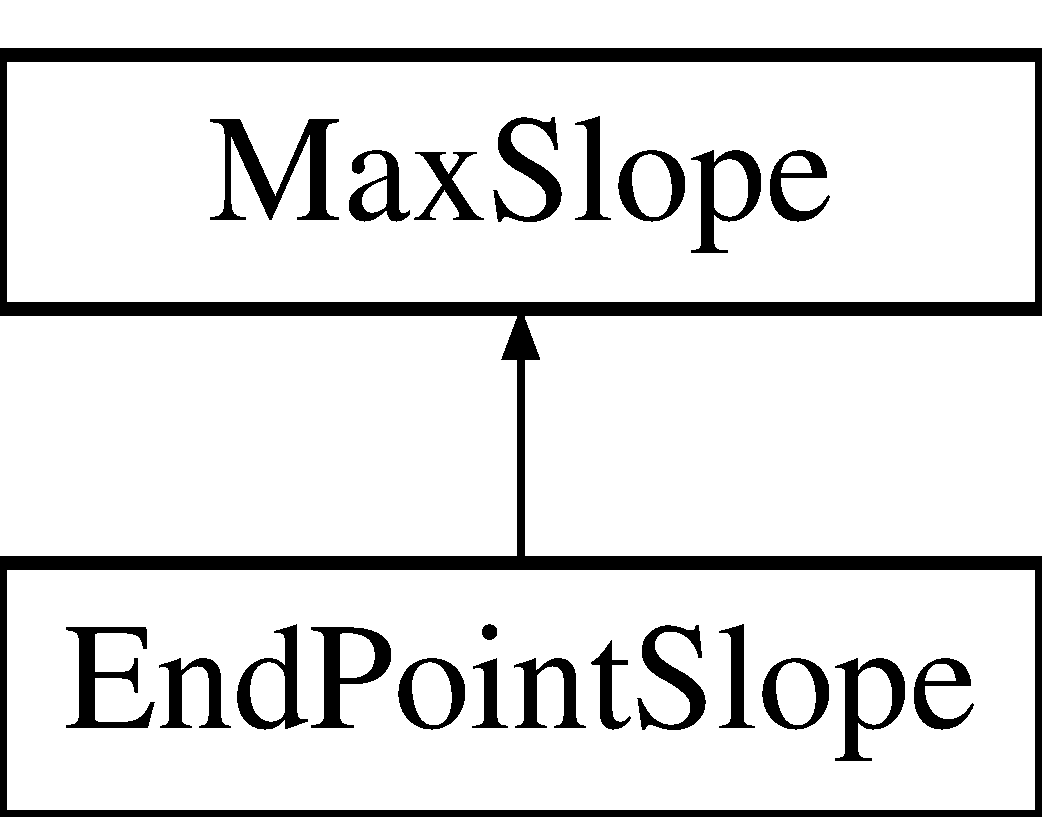
\includegraphics[height=2cm]{da/d7d/classEndPointSlope}
\end{center}
\end{figure}
\subsection*{Public Member Functions}
\begin{DoxyCompactItemize}
\item 
\hyperlink{classEndPointSlope_aa1c680c5137b40a465d2433e636892ce}{EndPointSlope} (const \hyperlink{classMatrix}{Matrix} \&progVar)
\begin{DoxyCompactList}\small\item\em Constructor. \item\end{DoxyCompactList}\item 
\hypertarget{classEndPointSlope_a37cf0a75d426b64fc50a8a76f45beb1f}{
\hyperlink{classEndPointSlope_a37cf0a75d426b64fc50a8a76f45beb1f}{$\sim$EndPointSlope} ()}
\label{da/d7d/classEndPointSlope_a37cf0a75d426b64fc50a8a76f45beb1f}

\begin{DoxyCompactList}\small\item\em Destructor. \item\end{DoxyCompactList}\item 
int \hyperlink{classEndPointSlope_a70417721fe8a60669a67d19a7855bef5}{MostMonotonic} (int $\ast$monoAry, const int ncols, const int col)
\begin{DoxyCompactList}\small\item\em Method to find the most monotonic progress variable. \item\end{DoxyCompactList}\end{DoxyCompactItemize}


\subsection{Constructor \& Destructor Documentation}
\hypertarget{classEndPointSlope_aa1c680c5137b40a465d2433e636892ce}{
\index{EndPointSlope@{EndPointSlope}!EndPointSlope@{EndPointSlope}}
\index{EndPointSlope@{EndPointSlope}!EndPointSlope@{EndPointSlope}}
\subsubsection[{EndPointSlope}]{\setlength{\rightskip}{0pt plus 5cm}EndPointSlope::EndPointSlope (const {\bf Matrix} \& {\em progVar})}}
\label{da/d7d/classEndPointSlope_aa1c680c5137b40a465d2433e636892ce}


Constructor. \hyperlink{classEndPointSlope}{EndPointSlope} is a class that determines the most monotonic progress variable with respect to temperature (or another specified column). It calculates the slope from the first and last endpoints of each progress variable column and selects the progress variable with the largest magnitude slope.

The slope is given by $ \frac{C_i(N) - C_i(1)}{N} $ 

\subsection{Member Function Documentation}
\hypertarget{classEndPointSlope_a70417721fe8a60669a67d19a7855bef5}{
\index{EndPointSlope@{EndPointSlope}!MostMonotonic@{MostMonotonic}}
\index{MostMonotonic@{MostMonotonic}!EndPointSlope@{EndPointSlope}}
\subsubsection[{MostMonotonic}]{\setlength{\rightskip}{0pt plus 5cm}int EndPointSlope::MostMonotonic (int $\ast$ {\em monoAry}, \/  const int {\em ncols}, \/  const int {\em col})\hspace{0.3cm}{\ttfamily  \mbox{[}virtual\mbox{]}}}}
\label{da/d7d/classEndPointSlope_a70417721fe8a60669a67d19a7855bef5}


Method to find the most monotonic progress variable. MostMonotonic calculates the slope of the best linear approximation for each progress variable which is strictly increasing or strictly decreasing. The output array monoAry must be of length ncols, where each cell holds a value of 3 if C is strictly monotonic and has the largest slope, 2 if C is strictly monotonic but does not have the largest slope, and 0 for non-\/monotonic C. col is the reference column.

\begin{DoxyVerb}
INPUTS:

int *monoAry       array containing integer flags that denote the monotonicity of candidate progress variables

const int ncols    number of columns of monoAry

const int col      the reference column

OUTPUT:

int                flag specifying whether or not the function succeeded 
                    = 0: success
		   != 0: something went wrong 
\end{DoxyVerb}
 

Implements \hyperlink{classMaxSlope}{MaxSlope}.

The documentation for this class was generated from the following files:\begin{DoxyCompactItemize}
\item 
src/endpointslope.h\item 
src/endpointslope.cc\end{DoxyCompactItemize}

\hypertarget{classmaxslope_1_1EndPointSlope}{
\section{maxslope::EndPointSlope Class Reference}
\label{d5/d36/classmaxslope_1_1EndPointSlope}\index{maxslope::EndPointSlope@{maxslope::EndPointSlope}}
}
Inheritance diagram for maxslope::EndPointSlope::\begin{figure}[H]
\begin{center}
\leavevmode
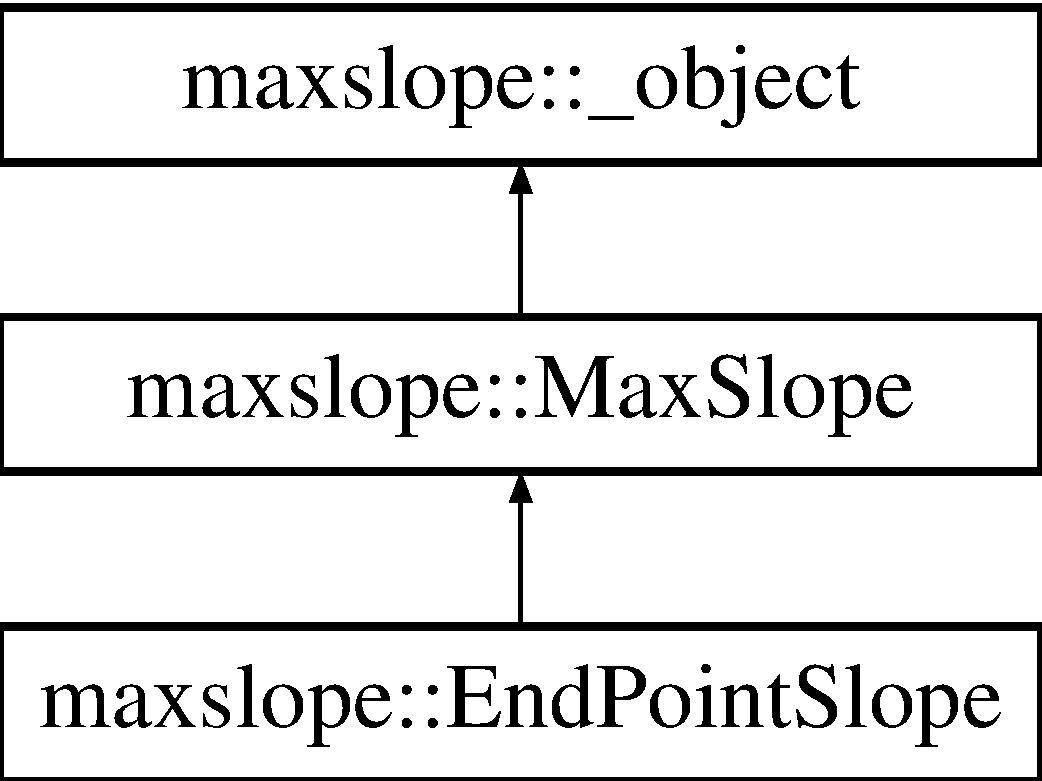
\includegraphics[height=3cm]{d5/d36/classmaxslope_1_1EndPointSlope}
\end{center}
\end{figure}
\subsection*{Public Member Functions}
\begin{DoxyCompactItemize}
\item 
\hypertarget{classmaxslope_1_1EndPointSlope_aa64ffcafb99bb6f9978a9037f14a18db}{
def {\bfseries \_\-\_\-init\_\-\_\-}}
\label{d5/d36/classmaxslope_1_1EndPointSlope_aa64ffcafb99bb6f9978a9037f14a18db}

\item 
\hypertarget{classmaxslope_1_1EndPointSlope_ac9ac444eccb64b1489ddf729975cb201}{
def {\bfseries MostMonotonic}}
\label{d5/d36/classmaxslope_1_1EndPointSlope_ac9ac444eccb64b1489ddf729975cb201}

\end{DoxyCompactItemize}
\subsection*{Public Attributes}
\begin{DoxyCompactItemize}
\item 
\hypertarget{classmaxslope_1_1EndPointSlope_ac09aca88eb1acd43cdfe6292862a3de1}{
{\bfseries this}}
\label{d5/d36/classmaxslope_1_1EndPointSlope_ac09aca88eb1acd43cdfe6292862a3de1}

\end{DoxyCompactItemize}


The documentation for this class was generated from the following file:\begin{DoxyCompactItemize}
\item 
src/maxslope.py\end{DoxyCompactItemize}

\hypertarget{classGLQuad}{
\section{GLQuad Class Reference}
\label{db/d06/classGLQuad}\index{GLQuad@{GLQuad}}
}
Inheritance diagram for GLQuad::\begin{figure}[H]
\begin{center}
\leavevmode
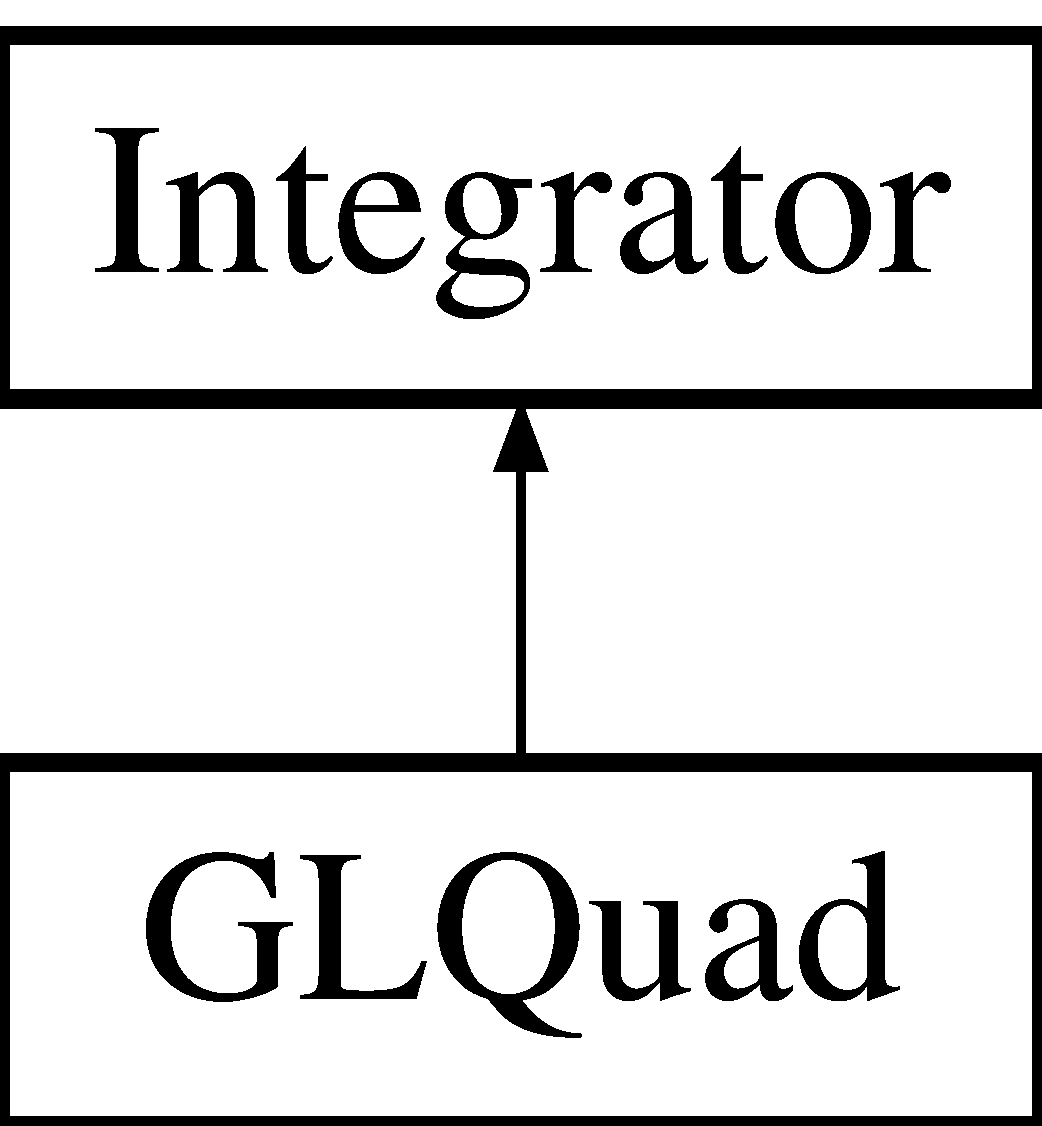
\includegraphics[height=2cm]{db/d06/classGLQuad}
\end{center}
\end{figure}
\subsection*{Public Member Functions}
\begin{DoxyCompactItemize}
\item 
\hypertarget{classGLQuad_a835d29af2507b6b2716794d3371d2ba8}{
{\bfseries GLQuad} (int Nodes)}
\label{db/d06/classGLQuad_a835d29af2507b6b2716794d3371d2ba8}

\item 
\hypertarget{classGLQuad_a951e36d849cfadc749a62218212802b6}{
double \hyperlink{classGLQuad_a951e36d849cfadc749a62218212802b6}{integrate} (const double $\ast$integrand, const double $\ast$Z, const int ZPoints)}
\label{db/d06/classGLQuad_a951e36d849cfadc749a62218212802b6}

\begin{DoxyCompactList}\small\item\em Virtual function to be inherited by each integration algorithm to integrate the given data set. \item\end{DoxyCompactList}\end{DoxyCompactItemize}


The documentation for this class was generated from the following files:\begin{DoxyCompactItemize}
\item 
src/glquad.h\item 
src/glquad.cc\end{DoxyCompactItemize}

\hypertarget{classintegrator_1_1GLQuad}{
\section{integrator::GLQuad Class Reference}
\label{d0/de8/classintegrator_1_1GLQuad}\index{integrator::GLQuad@{integrator::GLQuad}}
}
Inheritance diagram for integrator::GLQuad::\begin{figure}[H]
\begin{center}
\leavevmode
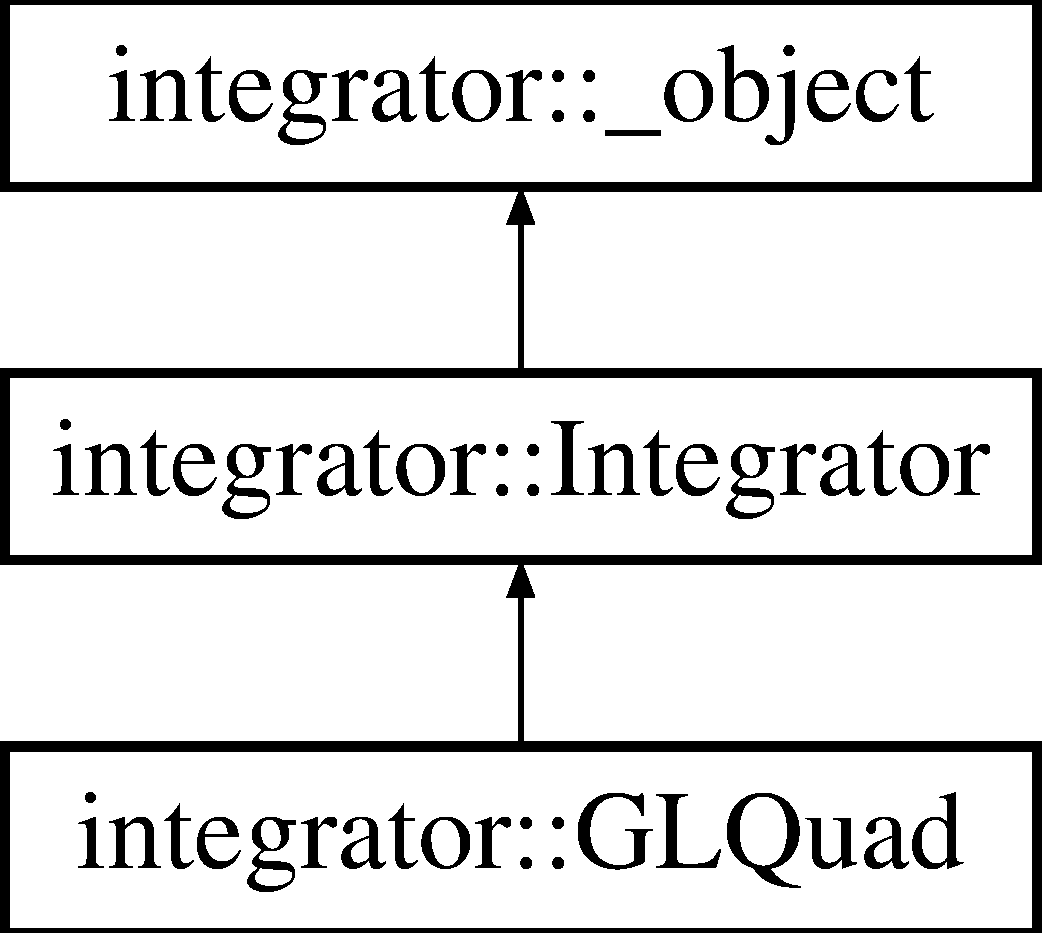
\includegraphics[height=3cm]{d0/de8/classintegrator_1_1GLQuad}
\end{center}
\end{figure}
\subsection*{Public Member Functions}
\begin{DoxyCompactItemize}
\item 
\hypertarget{classintegrator_1_1GLQuad_af1c5b397ad095a34096db39e83602ec9}{
def {\bfseries \_\-\_\-init\_\-\_\-}}
\label{d0/de8/classintegrator_1_1GLQuad_af1c5b397ad095a34096db39e83602ec9}

\item 
\hypertarget{classintegrator_1_1GLQuad_a85a93767e974c0890fe49e3811209cb4}{
def {\bfseries integrate}}
\label{d0/de8/classintegrator_1_1GLQuad_a85a93767e974c0890fe49e3811209cb4}

\end{DoxyCompactItemize}
\subsection*{Public Attributes}
\begin{DoxyCompactItemize}
\item 
\hypertarget{classintegrator_1_1GLQuad_a613996b0a038da751fa6cf2753d921cd}{
{\bfseries this}}
\label{d0/de8/classintegrator_1_1GLQuad_a613996b0a038da751fa6cf2753d921cd}

\end{DoxyCompactItemize}


The documentation for this class was generated from the following file:\begin{DoxyCompactItemize}
\item 
src/integrator.py\end{DoxyCompactItemize}

\hypertarget{classIntegrator}{
\section{Integrator Class Reference}
\label{da/d05/classIntegrator}\index{Integrator@{Integrator}}
}
Inheritance diagram for Integrator::\begin{figure}[H]
\begin{center}
\leavevmode
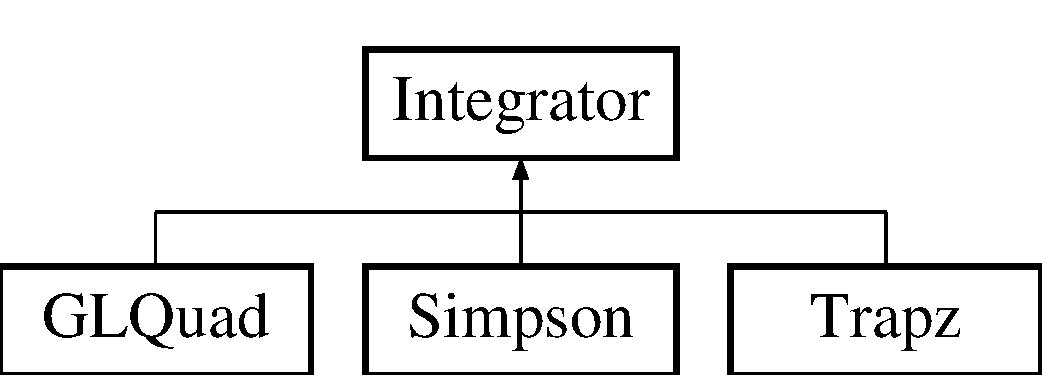
\includegraphics[height=2cm]{da/d05/classIntegrator}
\end{center}
\end{figure}
\subsection*{Public Member Functions}
\begin{DoxyCompactItemize}
\item 
\hypertarget{classIntegrator_a89fbef2f7923ce4e2c979b2ff1d1f4ac}{
virtual double {\bfseries integrate} (const double $\ast$integrand, const double $\ast$Z, const int ZPoints)=0}
\label{da/d05/classIntegrator_a89fbef2f7923ce4e2c979b2ff1d1f4ac}

\end{DoxyCompactItemize}


The documentation for this class was generated from the following file:\begin{DoxyCompactItemize}
\item 
src/integrator.h\end{DoxyCompactItemize}

\hypertarget{classintegrator_1_1Integrator}{
\section{integrator::Integrator Class Reference}
\label{dc/da1/classintegrator_1_1Integrator}\index{integrator::Integrator@{integrator::Integrator}}
}
Inheritance diagram for integrator::Integrator::\begin{figure}[H]
\begin{center}
\leavevmode
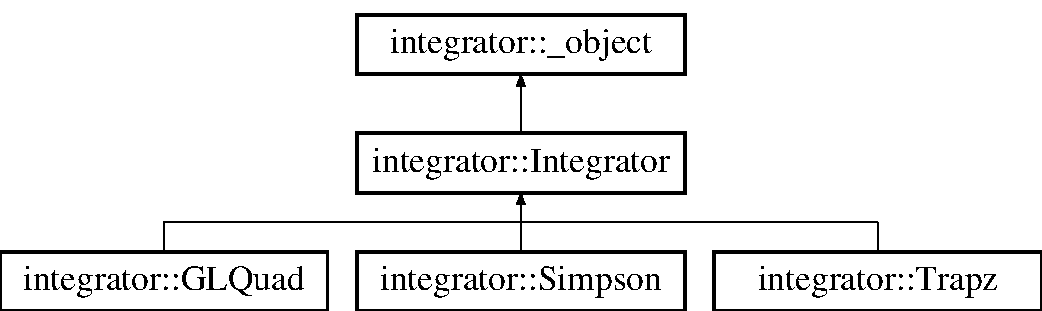
\includegraphics[height=3cm]{dc/da1/classintegrator_1_1Integrator}
\end{center}
\end{figure}
\subsection*{Public Member Functions}
\begin{DoxyCompactItemize}
\item 
\hypertarget{classintegrator_1_1Integrator_a973f474b13cde1d131d4a187b6b9f498}{
def {\bfseries \_\-\_\-init\_\-\_\-}}
\label{dc/da1/classintegrator_1_1Integrator_a973f474b13cde1d131d4a187b6b9f498}

\item 
\hypertarget{classintegrator_1_1Integrator_a7ab4e9c4f500e5c1020508e160237e0e}{
def {\bfseries integrate}}
\label{dc/da1/classintegrator_1_1Integrator_a7ab4e9c4f500e5c1020508e160237e0e}

\end{DoxyCompactItemize}


The documentation for this class was generated from the following file:\begin{DoxyCompactItemize}
\item 
src/integrator.py\end{DoxyCompactItemize}

\hypertarget{classlininterp_1_1Interpolator}{
\section{lininterp::Interpolator Class Reference}
\label{d4/de4/classlininterp_1_1Interpolator}\index{lininterp::Interpolator@{lininterp::Interpolator}}
}
Inheritance diagram for lininterp::Interpolator::\begin{figure}[H]
\begin{center}
\leavevmode
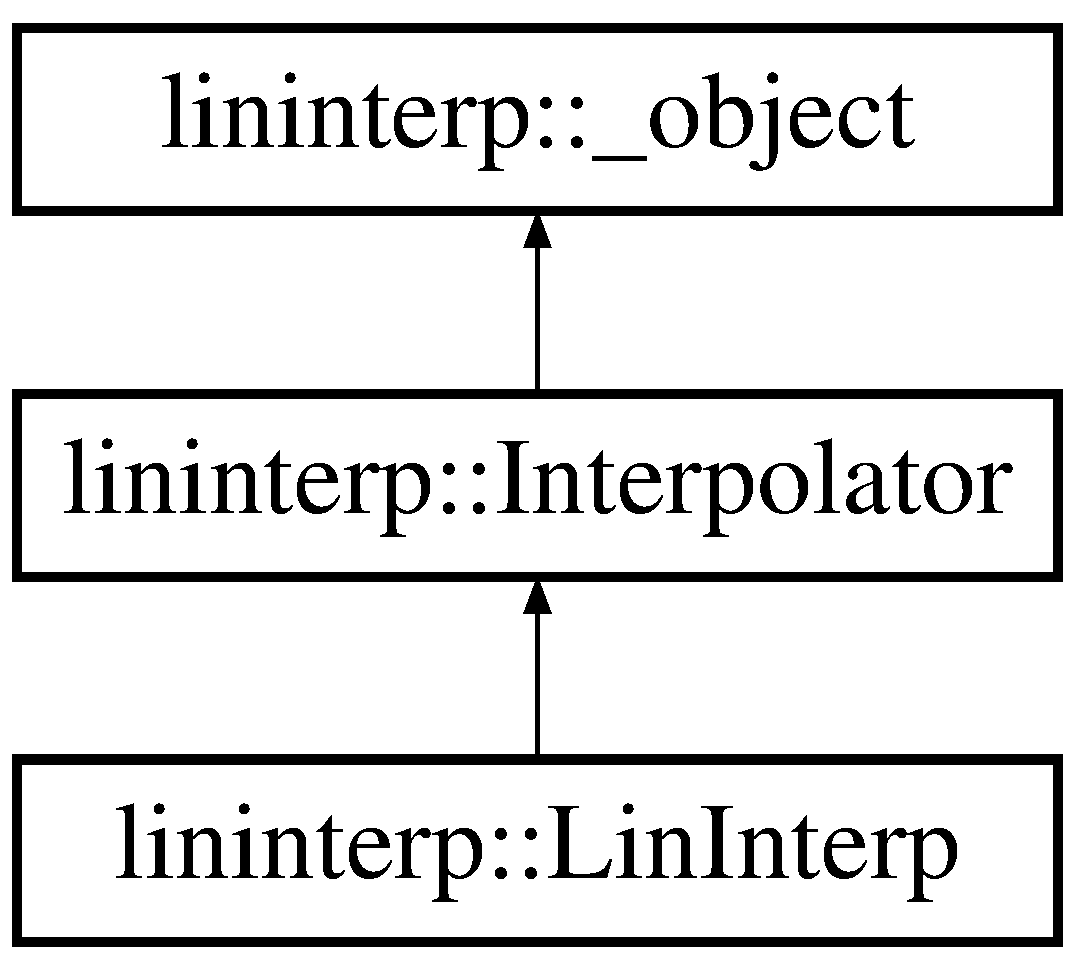
\includegraphics[height=3cm]{d4/de4/classlininterp_1_1Interpolator}
\end{center}
\end{figure}
\subsection*{Public Member Functions}
\begin{DoxyCompactItemize}
\item 
\hypertarget{classlininterp_1_1Interpolator_a0c338598d52dedcaa004534838ba2073}{
def {\bfseries \_\-\_\-init\_\-\_\-}}
\label{d4/de4/classlininterp_1_1Interpolator_a0c338598d52dedcaa004534838ba2073}

\item 
\hypertarget{classlininterp_1_1Interpolator_a6a32134abe67a61c3245c704793e95af}{
def {\bfseries Interp}}
\label{d4/de4/classlininterp_1_1Interpolator_a6a32134abe67a61c3245c704793e95af}

\end{DoxyCompactItemize}


The documentation for this class was generated from the following file:\begin{DoxyCompactItemize}
\item 
src/lininterp.py\end{DoxyCompactItemize}

\hypertarget{classInterpolator}{
\section{Interpolator Class Reference}
\label{d3/df3/classInterpolator}\index{Interpolator@{Interpolator}}
}
Inheritance diagram for Interpolator::\begin{figure}[H]
\begin{center}
\leavevmode
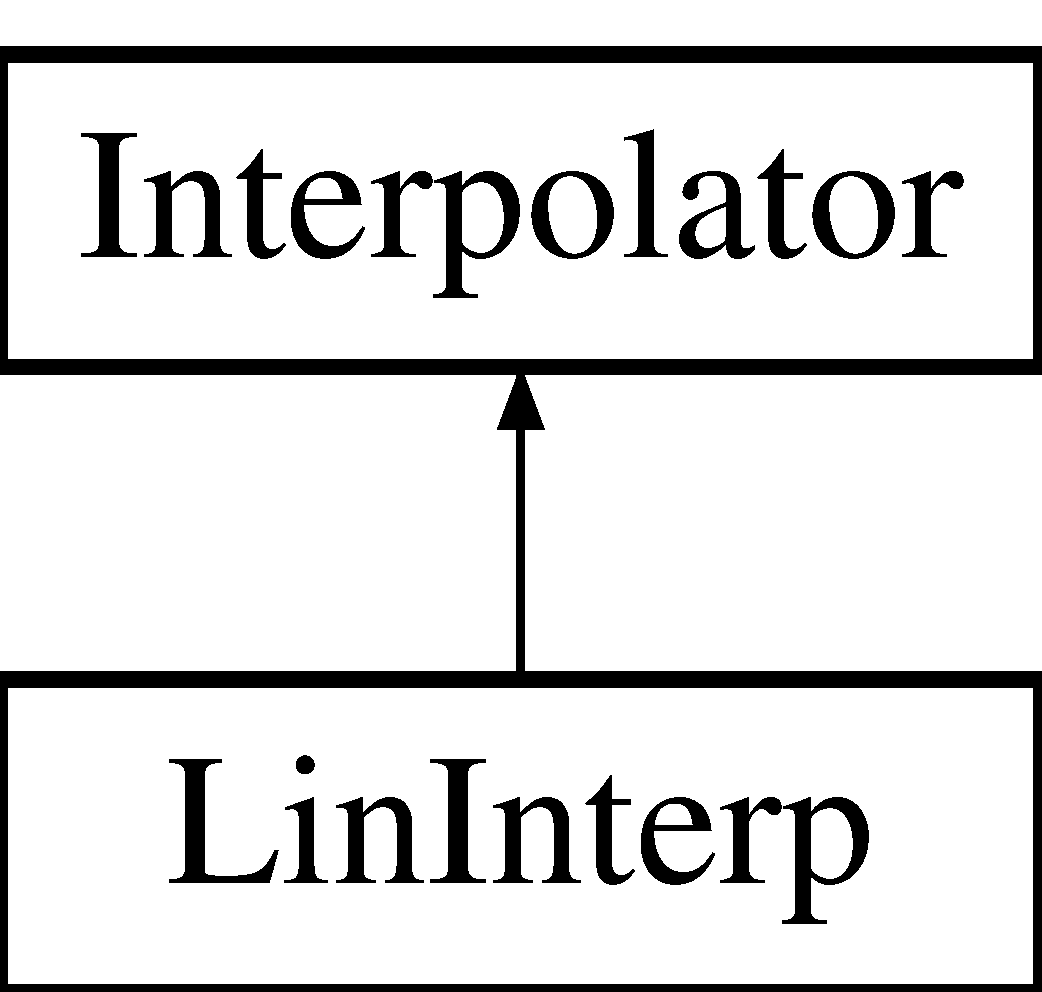
\includegraphics[height=2cm]{d3/df3/classInterpolator}
\end{center}
\end{figure}
\subsection*{Public Member Functions}
\begin{DoxyCompactItemize}
\item 
\hypertarget{classInterpolator_a2238defccb009047f624bda33cc47c73}{
virtual int {\bfseries Interp} (const \hyperlink{classMatrix}{Matrix} $\ast$matin, int col, double ival, double $\ast$vecout, int cols)=0}
\label{d3/df3/classInterpolator_a2238defccb009047f624bda33cc47c73}

\end{DoxyCompactItemize}


The documentation for this class was generated from the following file:\begin{DoxyCompactItemize}
\item 
src/interpolator.h\end{DoxyCompactItemize}

\hypertarget{classLeastNonMono}{
\section{LeastNonMono Class Reference}
\label{d9/da9/classLeastNonMono}\index{LeastNonMono@{LeastNonMono}}
}
Inheritance diagram for LeastNonMono::\begin{figure}[H]
\begin{center}
\leavevmode
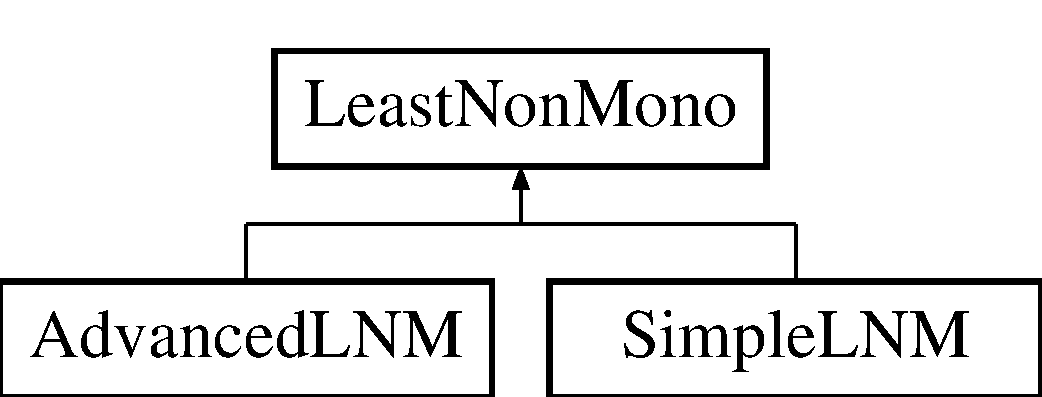
\includegraphics[height=2cm]{d9/da9/classLeastNonMono}
\end{center}
\end{figure}
\subsection*{Public Member Functions}
\begin{DoxyCompactItemize}
\item 
\hypertarget{classLeastNonMono_a239cbd7836950dc7c758138c4db00d0c}{
virtual int \hyperlink{classLeastNonMono_a239cbd7836950dc7c758138c4db00d0c}{LeastNonMonotonic} (int $\ast$monoAry, const int ncols, const int col)=0}
\label{d9/da9/classLeastNonMono_a239cbd7836950dc7c758138c4db00d0c}

\begin{DoxyCompactList}\small\item\em Virtual function to be inherited by each monotonicity cheking algorithm to determine the least non-\/monotonic progress variable. \item\end{DoxyCompactList}\end{DoxyCompactItemize}


The documentation for this class was generated from the following file:\begin{DoxyCompactItemize}
\item 
src/leastnonmono.h\end{DoxyCompactItemize}

\hypertarget{classleastnonmono_1_1LeastNonMono}{
\section{leastnonmono::LeastNonMono Class Reference}
\label{da/d81/classleastnonmono_1_1LeastNonMono}\index{leastnonmono::LeastNonMono@{leastnonmono::LeastNonMono}}
}
Inheritance diagram for leastnonmono::LeastNonMono::\begin{figure}[H]
\begin{center}
\leavevmode
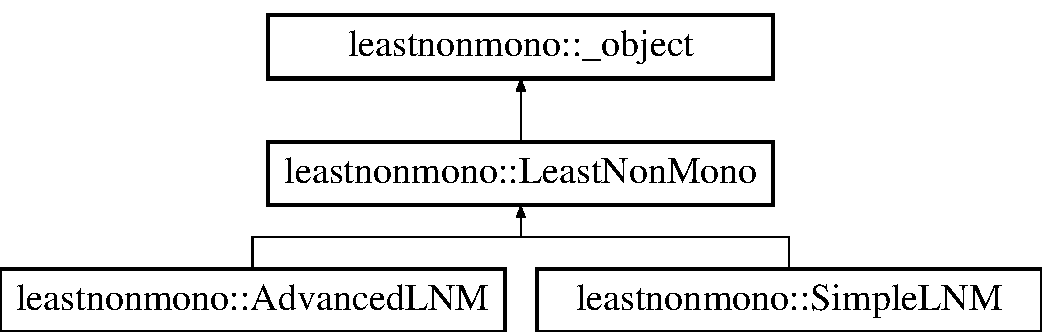
\includegraphics[height=3cm]{da/d81/classleastnonmono_1_1LeastNonMono}
\end{center}
\end{figure}
\subsection*{Public Member Functions}
\begin{DoxyCompactItemize}
\item 
\hypertarget{classleastnonmono_1_1LeastNonMono_ad27a656979919a3cf13907470b53fc2d}{
def {\bfseries \_\-\_\-init\_\-\_\-}}
\label{da/d81/classleastnonmono_1_1LeastNonMono_ad27a656979919a3cf13907470b53fc2d}

\item 
\hypertarget{classleastnonmono_1_1LeastNonMono_ab1899f44db61835de8d8f819a07bf07d}{
def {\bfseries LeastNonMonotonic}}
\label{da/d81/classleastnonmono_1_1LeastNonMono_ab1899f44db61835de8d8f819a07bf07d}

\end{DoxyCompactItemize}


The documentation for this class was generated from the following file:\begin{DoxyCompactItemize}
\item 
src/leastnonmono.py\end{DoxyCompactItemize}

\hypertarget{classlininterp_1_1LinInterp}{
\section{lininterp::LinInterp Class Reference}
\label{db/da6/classlininterp_1_1LinInterp}\index{lininterp::LinInterp@{lininterp::LinInterp}}
}
Inheritance diagram for lininterp::LinInterp::\begin{figure}[H]
\begin{center}
\leavevmode
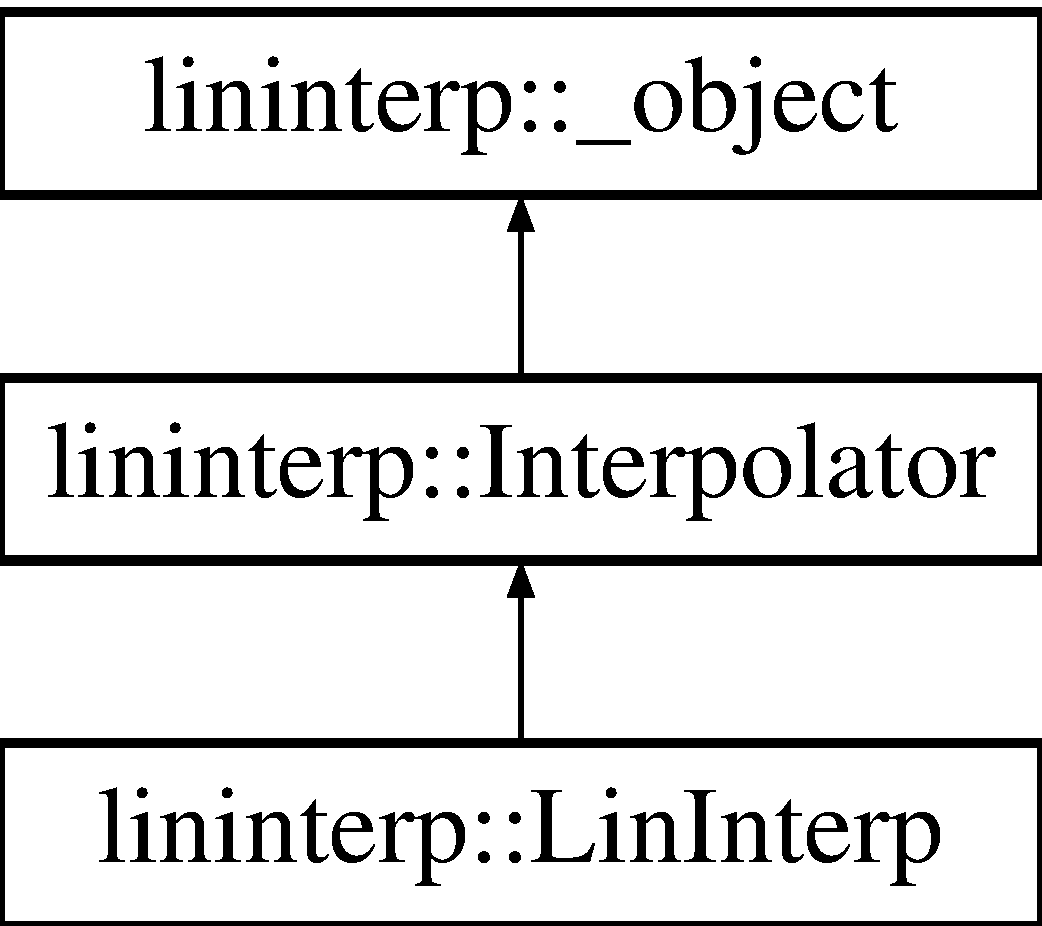
\includegraphics[height=3cm]{db/da6/classlininterp_1_1LinInterp}
\end{center}
\end{figure}
\subsection*{Public Member Functions}
\begin{DoxyCompactItemize}
\item 
\hypertarget{classlininterp_1_1LinInterp_ac3e5644b61ba0c4a406e5b9c4df73015}{
def {\bfseries \_\-\_\-init\_\-\_\-}}
\label{db/da6/classlininterp_1_1LinInterp_ac3e5644b61ba0c4a406e5b9c4df73015}

\item 
\hypertarget{classlininterp_1_1LinInterp_a2a0d4d4f60b4266c7c69307d5f8a03df}{
def {\bfseries Interp}}
\label{db/da6/classlininterp_1_1LinInterp_a2a0d4d4f60b4266c7c69307d5f8a03df}

\end{DoxyCompactItemize}
\subsection*{Public Attributes}
\begin{DoxyCompactItemize}
\item 
\hypertarget{classlininterp_1_1LinInterp_a2991116f7ec800a41b328bd1c4e71e6e}{
{\bfseries this}}
\label{db/da6/classlininterp_1_1LinInterp_a2991116f7ec800a41b328bd1c4e71e6e}

\end{DoxyCompactItemize}


The documentation for this class was generated from the following file:\begin{DoxyCompactItemize}
\item 
src/lininterp.py\end{DoxyCompactItemize}

\hypertarget{classLinInterp}{
\section{LinInterp Class Reference}
\label{d8/dee/classLinInterp}\index{LinInterp@{LinInterp}}
}
Inheritance diagram for LinInterp::\begin{figure}[H]
\begin{center}
\leavevmode
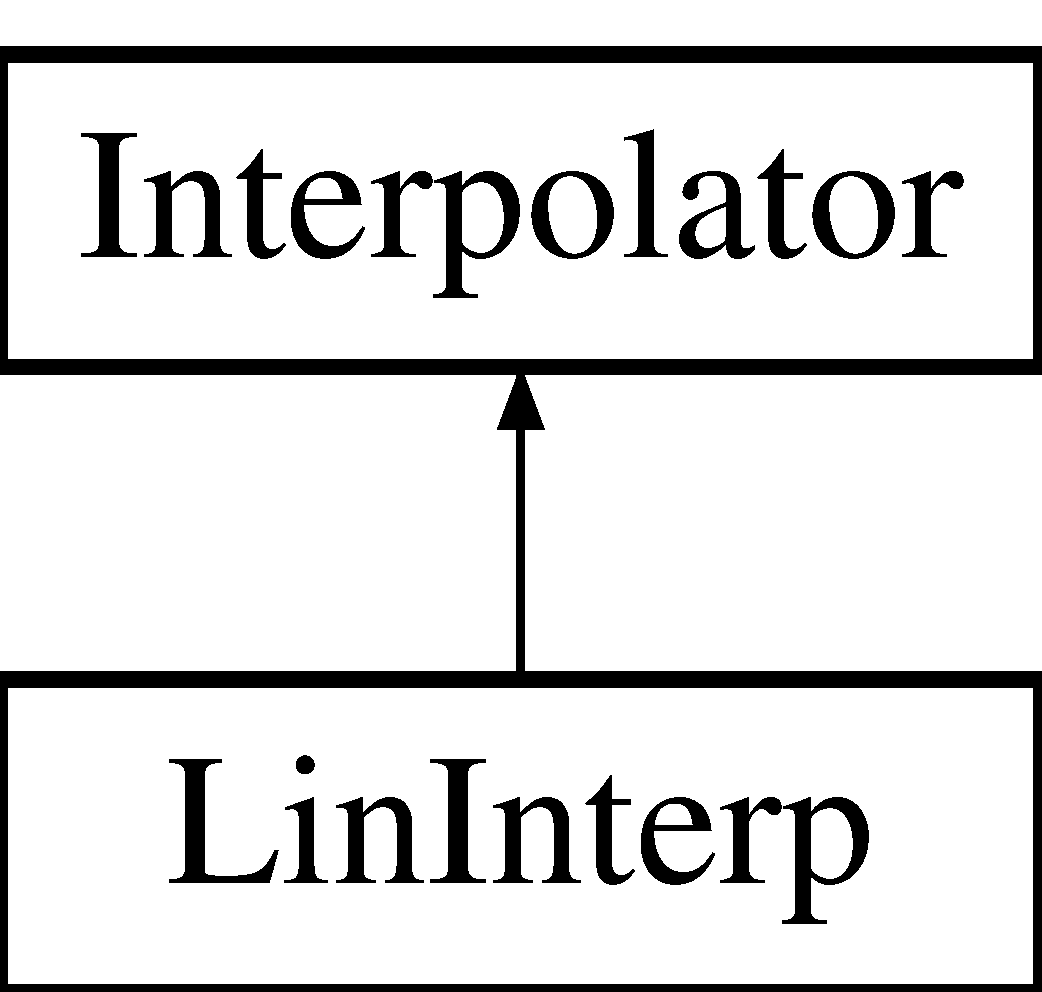
\includegraphics[height=2cm]{d8/dee/classLinInterp}
\end{center}
\end{figure}
\subsection*{Public Member Functions}
\begin{DoxyCompactItemize}
\item 
\hypertarget{classLinInterp_a56a58464dae6196cc671749133f1de12}{
\hyperlink{classLinInterp_a56a58464dae6196cc671749133f1de12}{LinInterp} ()}
\label{d8/dee/classLinInterp_a56a58464dae6196cc671749133f1de12}

\begin{DoxyCompactList}\small\item\em Constructor. \item\end{DoxyCompactList}\item 
\hypertarget{classLinInterp_a301177227b3013bcf9ea45e1c66fc468}{
\hyperlink{classLinInterp_a301177227b3013bcf9ea45e1c66fc468}{$\sim$LinInterp} ()}
\label{d8/dee/classLinInterp_a301177227b3013bcf9ea45e1c66fc468}

\begin{DoxyCompactList}\small\item\em Destructor. \item\end{DoxyCompactList}\item 
int \hyperlink{classLinInterp_a26aeb03c387bf5c8ea5db0ed111b5cd7}{Interp} (const \hyperlink{classMatrix}{Matrix} $\ast$matin, int col, double ival, double $\ast$vecout, int cols)
\begin{DoxyCompactList}\small\item\em Linear interpolation function. \item\end{DoxyCompactList}\end{DoxyCompactItemize}


\subsection{Member Function Documentation}
\hypertarget{classLinInterp_a26aeb03c387bf5c8ea5db0ed111b5cd7}{
\index{LinInterp@{LinInterp}!Interp@{Interp}}
\index{Interp@{Interp}!LinInterp@{LinInterp}}
\subsubsection[{Interp}]{\setlength{\rightskip}{0pt plus 5cm}int LinInterp::Interp (const {\bf Matrix} $\ast$ {\em matin}, \/  int {\em col}, \/  double {\em ival}, \/  double $\ast$ {\em vecout}, \/  int {\em cols})\hspace{0.3cm}{\ttfamily  \mbox{[}virtual\mbox{]}}}}
\label{d8/dee/classLinInterp_a26aeb03c387bf5c8ea5db0ed111b5cd7}


Linear interpolation function. This function takes in a 2D matrix of data and interpolates an entire row from it using a linear interpolator. Each column of the matrix is treated as a variable, with a specified column being the independent variable. The input data is not assumed to be sorted.

\begin{DoxyVerb}
  INPUTS:

  const Matrix *matin    pointer to a Matrix object. This is the input data.

  int col                integer specifying which column of the input Matrix is the independent 
                         variable

  double ival            value at which to interpolate

  double *vecout         pointer to an array which contains the interpolated row. This array has
                         the same number of columns as the input Matrix.

  int cols               number of columns of matin/vecout


  OUTPUTS:

  int                    flag specifying whether or not the function succeeded
                         = 0: success
			 = 1: extrapolation attempted
\end{DoxyVerb}
 

Implements \hyperlink{classInterpolator_a2238defccb009047f624bda33cc47c73}{Interpolator}.

The documentation for this class was generated from the following files:\begin{DoxyCompactItemize}
\item 
src/lininterp.h\item 
src/lininterp.cc\end{DoxyCompactItemize}

\hypertarget{classLinRegression}{
\section{LinRegression Class Reference}
\label{de/d89/classLinRegression}\index{LinRegression@{LinRegression}}
}
Inheritance diagram for LinRegression::\begin{figure}[H]
\begin{center}
\leavevmode
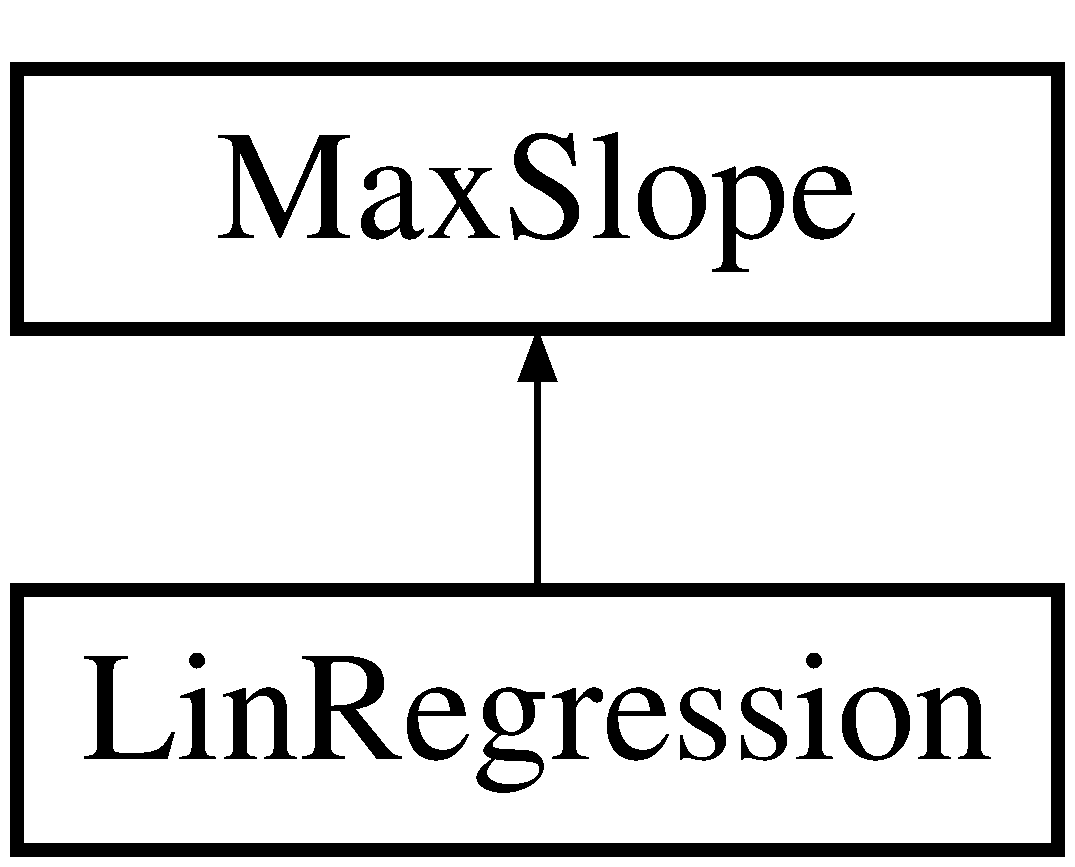
\includegraphics[height=2cm]{de/d89/classLinRegression}
\end{center}
\end{figure}
\subsection*{Public Member Functions}
\begin{DoxyCompactItemize}
\item 
\hyperlink{classLinRegression_a0d747e38f7a8997765be15f43062290c}{LinRegression} (const \hyperlink{classMatrix}{Matrix} \&progVar)
\begin{DoxyCompactList}\small\item\em Constructor. \item\end{DoxyCompactList}\item 
\hypertarget{classLinRegression_a4ea5ffb8032172bdf54d1f2d4041d520}{
\hyperlink{classLinRegression_a4ea5ffb8032172bdf54d1f2d4041d520}{$\sim$LinRegression} ()}
\label{de/d89/classLinRegression_a4ea5ffb8032172bdf54d1f2d4041d520}

\begin{DoxyCompactList}\small\item\em Destructor. \item\end{DoxyCompactList}\item 
int \hyperlink{classLinRegression_a1f245c4e47637f3f1d94f6129861406d}{MostMonotonic} (int $\ast$monoAry, const int ncols, const int col)
\begin{DoxyCompactList}\small\item\em Method to find the most monotonic progress variable. \item\end{DoxyCompactList}\end{DoxyCompactItemize}


\subsection{Constructor \& Destructor Documentation}
\hypertarget{classLinRegression_a0d747e38f7a8997765be15f43062290c}{
\index{LinRegression@{LinRegression}!LinRegression@{LinRegression}}
\index{LinRegression@{LinRegression}!LinRegression@{LinRegression}}
\subsubsection[{LinRegression}]{\setlength{\rightskip}{0pt plus 5cm}LinRegression::LinRegression (const {\bf Matrix} \& {\em progVar})}}
\label{de/d89/classLinRegression_a0d747e38f7a8997765be15f43062290c}


Constructor. \hyperlink{classLinRegression}{LinRegression} is a class that determines the most monotonic progress variable with respect to temperature (or another specified column). It calculates the slope of the best linear approximation for each progress variable and selects the largest magnitude.

The slope is given by \{sum\_\-i=1\_\-i=N (C\_\-i-\/C\_\-ave)(T\_\-i-\/T\_\-ave)\}/\{sum\_\-i=1\_\-i=N (T\_\-i-\/T\_\-ave)$^\wedge$2\} 

\subsection{Member Function Documentation}
\hypertarget{classLinRegression_a1f245c4e47637f3f1d94f6129861406d}{
\index{LinRegression@{LinRegression}!MostMonotonic@{MostMonotonic}}
\index{MostMonotonic@{MostMonotonic}!LinRegression@{LinRegression}}
\subsubsection[{MostMonotonic}]{\setlength{\rightskip}{0pt plus 5cm}int LinRegression::MostMonotonic (int $\ast$ {\em monoAry}, \/  const int {\em ncols}, \/  const int {\em col})\hspace{0.3cm}{\ttfamily  \mbox{[}virtual\mbox{]}}}}
\label{de/d89/classLinRegression_a1f245c4e47637f3f1d94f6129861406d}


Method to find the most monotonic progress variable. MostMonotonic calculates the slope of the best linear approximation for each progress variable which is strictly increasing or strictly decreasing. The output array monoAry must be of length ncols, where each cell holds a value of 3 if C is strictly monotonic and has the largest slope, 2 if C is strictly monotonic but does not have the largest slope, and 0 for non-\/monotonic C. col is the reference column. 

Implements \hyperlink{classMaxSlope_a494b1b1ae073d3b29fe7cdc023ce7861}{MaxSlope}.

The documentation for this class was generated from the following files:\begin{DoxyCompactItemize}
\item 
src/linregression.h\item 
src/linregression.cc\end{DoxyCompactItemize}

\hypertarget{classmaxslope_1_1LinRegression}{
\section{maxslope::LinRegression Class Reference}
\label{d4/dbe/classmaxslope_1_1LinRegression}\index{maxslope::LinRegression@{maxslope::LinRegression}}
}
Inheritance diagram for maxslope::LinRegression::\begin{figure}[H]
\begin{center}
\leavevmode
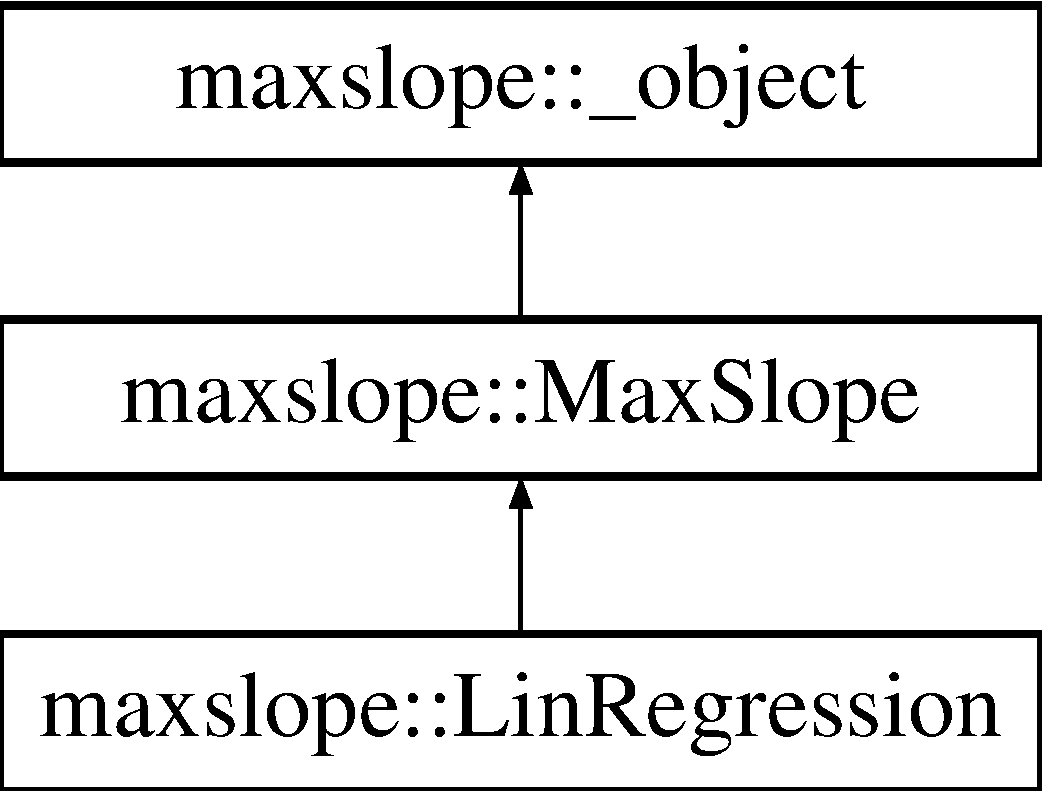
\includegraphics[height=3cm]{d4/dbe/classmaxslope_1_1LinRegression}
\end{center}
\end{figure}
\subsection*{Public Member Functions}
\begin{DoxyCompactItemize}
\item 
\hypertarget{classmaxslope_1_1LinRegression_ab45de3d79a109d5e052e219a102dbeec}{
def {\bfseries \_\-\_\-init\_\-\_\-}}
\label{d4/dbe/classmaxslope_1_1LinRegression_ab45de3d79a109d5e052e219a102dbeec}

\item 
\hypertarget{classmaxslope_1_1LinRegression_a963c3ebdaab1a12e99a6efc812de9226}{
def {\bfseries MostMonotonic}}
\label{d4/dbe/classmaxslope_1_1LinRegression_a963c3ebdaab1a12e99a6efc812de9226}

\end{DoxyCompactItemize}
\subsection*{Public Attributes}
\begin{DoxyCompactItemize}
\item 
\hypertarget{classmaxslope_1_1LinRegression_a359905ee6312345940c5ad51583acbc8}{
{\bfseries this}}
\label{d4/dbe/classmaxslope_1_1LinRegression_a359905ee6312345940c5ad51583acbc8}

\end{DoxyCompactItemize}


The documentation for this class was generated from the following file:\begin{DoxyCompactItemize}
\item 
src/maxslope.py\end{DoxyCompactItemize}

\hypertarget{classMatrix}{
\section{Matrix Class Reference}
\label{d3/d3f/classMatrix}\index{Matrix@{Matrix}}
}
\subsection*{Public Member Functions}
\begin{DoxyCompactItemize}
\item 
\hypertarget{classMatrix_a7213414e405fd1c81c394d5053721fa7}{
\hyperlink{classMatrix_a7213414e405fd1c81c394d5053721fa7}{Matrix} (int rows, int cols)}
\label{d3/d3f/classMatrix_a7213414e405fd1c81c394d5053721fa7}

\begin{DoxyCompactList}\small\item\em Constructor. \item\end{DoxyCompactList}\item 
\hypertarget{classMatrix_a9b1c3627f573d78a2f08623fdfef990f}{
\hyperlink{classMatrix_a9b1c3627f573d78a2f08623fdfef990f}{$\sim$Matrix} ()}
\label{d3/d3f/classMatrix_a9b1c3627f573d78a2f08623fdfef990f}

\begin{DoxyCompactList}\small\item\em Destructor. \item\end{DoxyCompactList}\item 
\hypertarget{classMatrix_ad7da71a311eeedf1ac24be5c6ada4dcb}{
double \hyperlink{classMatrix_ad7da71a311eeedf1ac24be5c6ada4dcb}{GetVal} (int i, int j) const }
\label{d3/d3f/classMatrix_ad7da71a311eeedf1ac24be5c6ada4dcb}

\begin{DoxyCompactList}\small\item\em Get the value at a specified index. \item\end{DoxyCompactList}\item 
\hypertarget{classMatrix_aa8c1c4e96ce2dff650a31dd0650db7db}{
void \hyperlink{classMatrix_aa8c1c4e96ce2dff650a31dd0650db7db}{SetVal} (int i, int j, double val)}
\label{d3/d3f/classMatrix_aa8c1c4e96ce2dff650a31dd0650db7db}

\begin{DoxyCompactList}\small\item\em Set the value at a specific location. \item\end{DoxyCompactList}\item 
\hypertarget{classMatrix_ae683a43cfb2cb84e8f6fa0297744b307}{
int \hyperlink{classMatrix_ae683a43cfb2cb84e8f6fa0297744b307}{GetNumRows} () const }
\label{d3/d3f/classMatrix_ae683a43cfb2cb84e8f6fa0297744b307}

\begin{DoxyCompactList}\small\item\em Return the number of rows. \item\end{DoxyCompactList}\item 
\hypertarget{classMatrix_a4069e97fcef57fce6828c6042d63e7d2}{
int \hyperlink{classMatrix_a4069e97fcef57fce6828c6042d63e7d2}{GetNumCols} () const }
\label{d3/d3f/classMatrix_a4069e97fcef57fce6828c6042d63e7d2}

\begin{DoxyCompactList}\small\item\em Return the number of columns. \item\end{DoxyCompactList}\item 
\hypertarget{classMatrix_a830c8a78828c4db552648e46aef5ec6e}{
int \hyperlink{classMatrix_a830c8a78828c4db552648e46aef5ec6e}{GetCol} (int j, double $\ast$colAry) const }
\label{d3/d3f/classMatrix_a830c8a78828c4db552648e46aef5ec6e}

\begin{DoxyCompactList}\small\item\em Return an array containing column j. \item\end{DoxyCompactList}\end{DoxyCompactItemize}


The documentation for this class was generated from the following files:\begin{DoxyCompactItemize}
\item 
src/matrix.h\item 
src/matrix.cc\end{DoxyCompactItemize}

\hypertarget{classmatrix_1_1Matrix}{
\section{matrix::Matrix Class Reference}
\label{dd/db9/classmatrix_1_1Matrix}\index{matrix::Matrix@{matrix::Matrix}}
}
Inheritance diagram for matrix::Matrix::\begin{figure}[H]
\begin{center}
\leavevmode
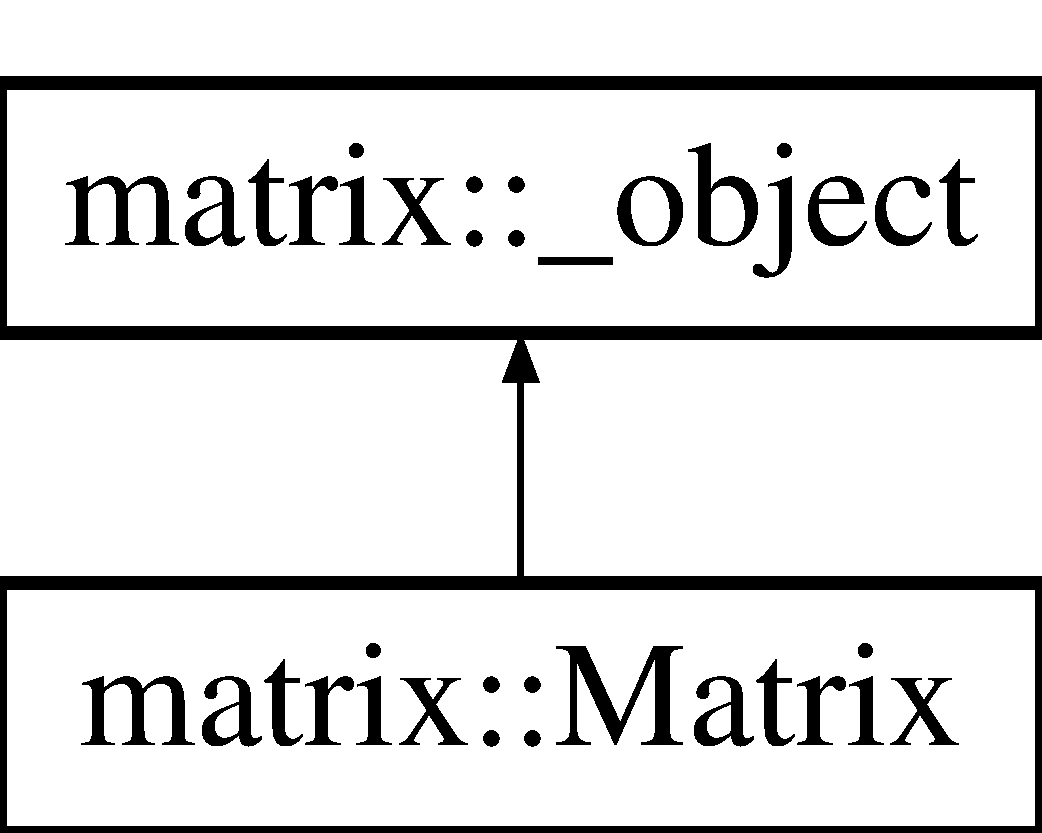
\includegraphics[height=2cm]{dd/db9/classmatrix_1_1Matrix}
\end{center}
\end{figure}
\subsection*{Public Member Functions}
\begin{DoxyCompactItemize}
\item 
\hypertarget{classmatrix_1_1Matrix_af668028ba2f2859741988054da60ee75}{
def {\bfseries \_\-\_\-init\_\-\_\-}}
\label{dd/db9/classmatrix_1_1Matrix_af668028ba2f2859741988054da60ee75}

\item 
\hypertarget{classmatrix_1_1Matrix_a78af2756e24b6f0d74695956b2f02646}{
def {\bfseries GetVal}}
\label{dd/db9/classmatrix_1_1Matrix_a78af2756e24b6f0d74695956b2f02646}

\item 
\hypertarget{classmatrix_1_1Matrix_ae7b5ee268f12fb34ebbbe7213f91638a}{
def {\bfseries SetVal}}
\label{dd/db9/classmatrix_1_1Matrix_ae7b5ee268f12fb34ebbbe7213f91638a}

\item 
\hypertarget{classmatrix_1_1Matrix_a25ad06ac9533ca524f9f17734d6a1ad6}{
def {\bfseries GetNumRows}}
\label{dd/db9/classmatrix_1_1Matrix_a25ad06ac9533ca524f9f17734d6a1ad6}

\item 
\hypertarget{classmatrix_1_1Matrix_af4ec3fb39dcbec6b92df554051019e6d}{
def {\bfseries GetNumCols}}
\label{dd/db9/classmatrix_1_1Matrix_af4ec3fb39dcbec6b92df554051019e6d}

\item 
\hypertarget{classmatrix_1_1Matrix_a81fd68a34b15d0f2412818b39eaaf02c}{
def {\bfseries GetCol}}
\label{dd/db9/classmatrix_1_1Matrix_a81fd68a34b15d0f2412818b39eaaf02c}

\end{DoxyCompactItemize}
\subsection*{Public Attributes}
\begin{DoxyCompactItemize}
\item 
\hypertarget{classmatrix_1_1Matrix_acc21534927e527008524f070e1a8f5fd}{
{\bfseries this}}
\label{dd/db9/classmatrix_1_1Matrix_acc21534927e527008524f070e1a8f5fd}

\end{DoxyCompactItemize}


The documentation for this class was generated from the following file:\begin{DoxyCompactItemize}
\item 
src/matrix.py\end{DoxyCompactItemize}

\hypertarget{classmonocheck_1_1Matrix}{
\section{monocheck::Matrix Class Reference}
\label{d3/d15/classmonocheck_1_1Matrix}\index{monocheck::Matrix@{monocheck::Matrix}}
}
Inheritance diagram for monocheck::Matrix::\begin{figure}[H]
\begin{center}
\leavevmode
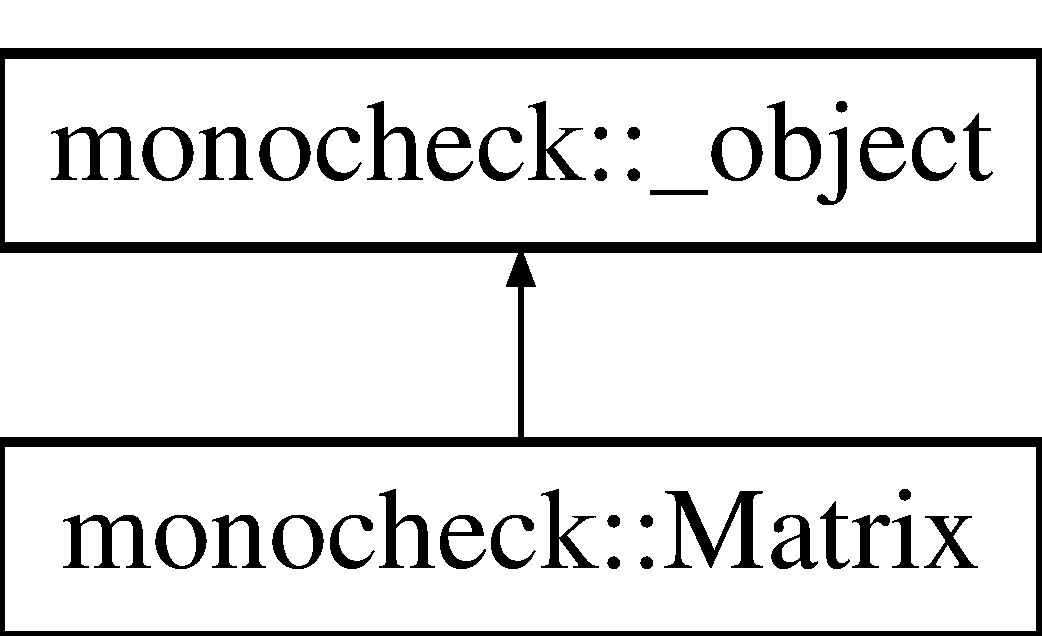
\includegraphics[height=2cm]{d3/d15/classmonocheck_1_1Matrix}
\end{center}
\end{figure}
\subsection*{Public Member Functions}
\begin{DoxyCompactItemize}
\item 
\hypertarget{classmonocheck_1_1Matrix_a24536d0f43c78981935dd94967a121cf}{
def {\bfseries \_\-\_\-init\_\-\_\-}}
\label{d3/d15/classmonocheck_1_1Matrix_a24536d0f43c78981935dd94967a121cf}

\item 
\hypertarget{classmonocheck_1_1Matrix_aa3a58278b48efcfff8e5c491b7f86b44}{
def {\bfseries GetVal}}
\label{d3/d15/classmonocheck_1_1Matrix_aa3a58278b48efcfff8e5c491b7f86b44}

\item 
\hypertarget{classmonocheck_1_1Matrix_ac3c442daf925b657fe290c72dae1271c}{
def {\bfseries SetVal}}
\label{d3/d15/classmonocheck_1_1Matrix_ac3c442daf925b657fe290c72dae1271c}

\item 
\hypertarget{classmonocheck_1_1Matrix_abdb690f5b480564be56ff839f6cd79e7}{
def {\bfseries GetNumRows}}
\label{d3/d15/classmonocheck_1_1Matrix_abdb690f5b480564be56ff839f6cd79e7}

\item 
\hypertarget{classmonocheck_1_1Matrix_afe4ec68e3ecf301292b417cc2daf1db3}{
def {\bfseries GetNumCols}}
\label{d3/d15/classmonocheck_1_1Matrix_afe4ec68e3ecf301292b417cc2daf1db3}

\item 
\hypertarget{classmonocheck_1_1Matrix_af023859e735f04776b64d225d58ec5a5}{
def {\bfseries GetCol}}
\label{d3/d15/classmonocheck_1_1Matrix_af023859e735f04776b64d225d58ec5a5}

\end{DoxyCompactItemize}
\subsection*{Public Attributes}
\begin{DoxyCompactItemize}
\item 
\hypertarget{classmonocheck_1_1Matrix_aaa81a06876b224d4caf8663c14444835}{
{\bfseries this}}
\label{d3/d15/classmonocheck_1_1Matrix_aaa81a06876b224d4caf8663c14444835}

\end{DoxyCompactItemize}


The documentation for this class was generated from the following file:\begin{DoxyCompactItemize}
\item 
src/monocheck.py\end{DoxyCompactItemize}

\hypertarget{classMatrix3D}{
\section{Matrix3D Class Reference}
\label{d0/dcb/classMatrix3D}\index{Matrix3D@{Matrix3D}}
}
\subsection*{Public Member Functions}
\begin{DoxyCompactItemize}
\item 
\hypertarget{classMatrix3D_a79ffea45e6ad9f5789f5444f033cb8f4}{
\hyperlink{classMatrix3D_a79ffea45e6ad9f5789f5444f033cb8f4}{Matrix3D} (int dim1, int dim2, int dim3)}
\label{d0/dcb/classMatrix3D_a79ffea45e6ad9f5789f5444f033cb8f4}

\begin{DoxyCompactList}\small\item\em Constructor. \item\end{DoxyCompactList}\item 
\hypertarget{classMatrix3D_a67ebf80ff62e71d327066491811401af}{
\hyperlink{classMatrix3D_a67ebf80ff62e71d327066491811401af}{$\sim$Matrix3D} ()}
\label{d0/dcb/classMatrix3D_a67ebf80ff62e71d327066491811401af}

\begin{DoxyCompactList}\small\item\em Destructor. \item\end{DoxyCompactList}\item 
\hypertarget{classMatrix3D_a8422daf16b13a3a26f3856dcadfae291}{
double \hyperlink{classMatrix3D_a8422daf16b13a3a26f3856dcadfae291}{GetVal} (int i, int j, int k) const }
\label{d0/dcb/classMatrix3D_a8422daf16b13a3a26f3856dcadfae291}

\begin{DoxyCompactList}\small\item\em Get the value at a specified index. \item\end{DoxyCompactList}\item 
\hypertarget{classMatrix3D_a082378ce9c6565d0655cb0ec2e68116c}{
void \hyperlink{classMatrix3D_a082378ce9c6565d0655cb0ec2e68116c}{SetVal} (int i, int j, int k, double vol)}
\label{d0/dcb/classMatrix3D_a082378ce9c6565d0655cb0ec2e68116c}

\begin{DoxyCompactList}\small\item\em Set the value at a specified index. \item\end{DoxyCompactList}\item 
\hypertarget{classMatrix3D_a97e904be2b5177157d7ecb11488c6ef3}{
int \hyperlink{classMatrix3D_a97e904be2b5177157d7ecb11488c6ef3}{GetNumDim1} () const }
\label{d0/dcb/classMatrix3D_a97e904be2b5177157d7ecb11488c6ef3}

\begin{DoxyCompactList}\small\item\em Return dim1. \item\end{DoxyCompactList}\item 
\hypertarget{classMatrix3D_ad6895586f9041457377a2b4e0b5778ce}{
int \hyperlink{classMatrix3D_ad6895586f9041457377a2b4e0b5778ce}{GetNumDim2} () const }
\label{d0/dcb/classMatrix3D_ad6895586f9041457377a2b4e0b5778ce}

\begin{DoxyCompactList}\small\item\em Return dim2. \item\end{DoxyCompactList}\item 
\hypertarget{classMatrix3D_aa98e87c6887afa3141cd290818650932}{
int \hyperlink{classMatrix3D_aa98e87c6887afa3141cd290818650932}{GetNumDim3} () const }
\label{d0/dcb/classMatrix3D_aa98e87c6887afa3141cd290818650932}

\begin{DoxyCompactList}\small\item\em Return dim3. \item\end{DoxyCompactList}\end{DoxyCompactItemize}


The documentation for this class was generated from the following files:\begin{DoxyCompactItemize}
\item 
src/matrix3d.h\item 
src/matrix3d.cc\end{DoxyCompactItemize}

\hypertarget{classmatrix3d_1_1Matrix3D}{
\section{matrix3d::Matrix3D Class Reference}
\label{d4/dbb/classmatrix3d_1_1Matrix3D}\index{matrix3d::Matrix3D@{matrix3d::Matrix3D}}
}
Inheritance diagram for matrix3d::Matrix3D::\begin{figure}[H]
\begin{center}
\leavevmode
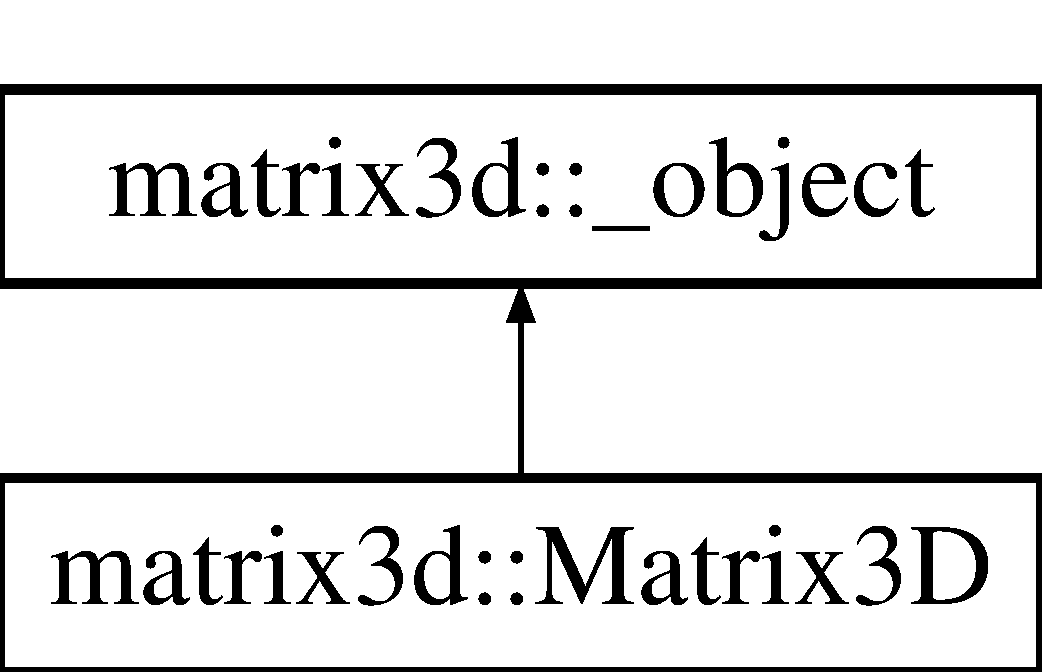
\includegraphics[height=2cm]{d4/dbb/classmatrix3d_1_1Matrix3D}
\end{center}
\end{figure}
\subsection*{Public Member Functions}
\begin{DoxyCompactItemize}
\item 
\hypertarget{classmatrix3d_1_1Matrix3D_afc828ef75c2d6fda473bab6673006fc2}{
def {\bfseries \_\-\_\-init\_\-\_\-}}
\label{d4/dbb/classmatrix3d_1_1Matrix3D_afc828ef75c2d6fda473bab6673006fc2}

\item 
\hypertarget{classmatrix3d_1_1Matrix3D_a9647e57d80350d7910056de98e6bfc2a}{
def {\bfseries GetVal}}
\label{d4/dbb/classmatrix3d_1_1Matrix3D_a9647e57d80350d7910056de98e6bfc2a}

\item 
\hypertarget{classmatrix3d_1_1Matrix3D_a1996596a1f5a693c6f8e320aef7b7710}{
def {\bfseries SetVal}}
\label{d4/dbb/classmatrix3d_1_1Matrix3D_a1996596a1f5a693c6f8e320aef7b7710}

\item 
\hypertarget{classmatrix3d_1_1Matrix3D_a6b2c6828d4b23fac9e5d73947cd8fd5c}{
def {\bfseries GetNumDim1}}
\label{d4/dbb/classmatrix3d_1_1Matrix3D_a6b2c6828d4b23fac9e5d73947cd8fd5c}

\item 
\hypertarget{classmatrix3d_1_1Matrix3D_a11ba8f2b438f400343f199d3eb858714}{
def {\bfseries GetNumDim2}}
\label{d4/dbb/classmatrix3d_1_1Matrix3D_a11ba8f2b438f400343f199d3eb858714}

\item 
\hypertarget{classmatrix3d_1_1Matrix3D_a23d415fad6978cae908870e45ebc30cc}{
def {\bfseries GetNumDim3}}
\label{d4/dbb/classmatrix3d_1_1Matrix3D_a23d415fad6978cae908870e45ebc30cc}

\end{DoxyCompactItemize}
\subsection*{Public Attributes}
\begin{DoxyCompactItemize}
\item 
\hypertarget{classmatrix3d_1_1Matrix3D_adb19e1ac1341d747d9f7a9e70e89f053}{
{\bfseries this}}
\label{d4/dbb/classmatrix3d_1_1Matrix3D_adb19e1ac1341d747d9f7a9e70e89f053}

\end{DoxyCompactItemize}


The documentation for this class was generated from the following file:\begin{DoxyCompactItemize}
\item 
src/matrix3d.py\end{DoxyCompactItemize}

\hypertarget{classMatrix4D}{
\section{Matrix4D Class Reference}
\label{d7/d9c/classMatrix4D}\index{Matrix4D@{Matrix4D}}
}
\subsection*{Public Member Functions}
\begin{DoxyCompactItemize}
\item 
\hypertarget{classMatrix4D_ac4ef4cb38ec681c8ae057081aa1235ef}{
\hyperlink{classMatrix4D_ac4ef4cb38ec681c8ae057081aa1235ef}{Matrix4D} (int dim1, int dim2, int dim3, int dim4)}
\label{d7/d9c/classMatrix4D_ac4ef4cb38ec681c8ae057081aa1235ef}

\begin{DoxyCompactList}\small\item\em Constructor. \item\end{DoxyCompactList}\item 
\hypertarget{classMatrix4D_a90b64981f087dfcb496b8f5a0449803c}{
\hyperlink{classMatrix4D_a90b64981f087dfcb496b8f5a0449803c}{$\sim$Matrix4D} ()}
\label{d7/d9c/classMatrix4D_a90b64981f087dfcb496b8f5a0449803c}

\begin{DoxyCompactList}\small\item\em Destructor. \item\end{DoxyCompactList}\item 
\hypertarget{classMatrix4D_a03f55155ae67a6741a662494ac7da18a}{
double \hyperlink{classMatrix4D_a03f55155ae67a6741a662494ac7da18a}{GetVal} (int i, int j, int k, int l) const }
\label{d7/d9c/classMatrix4D_a03f55155ae67a6741a662494ac7da18a}

\begin{DoxyCompactList}\small\item\em Get the value at a specified index. \item\end{DoxyCompactList}\item 
\hypertarget{classMatrix4D_a113ab746b94d6c253823f53cae3b8181}{
void \hyperlink{classMatrix4D_a113ab746b94d6c253823f53cae3b8181}{SetVal} (int i, int j, int k, int l, double val)}
\label{d7/d9c/classMatrix4D_a113ab746b94d6c253823f53cae3b8181}

\begin{DoxyCompactList}\small\item\em Set the value at a specified index. \item\end{DoxyCompactList}\item 
\hypertarget{classMatrix4D_a7582cae941bf64578b9099ad91afc869}{
int \hyperlink{classMatrix4D_a7582cae941bf64578b9099ad91afc869}{GetNumDim1} () const }
\label{d7/d9c/classMatrix4D_a7582cae941bf64578b9099ad91afc869}

\begin{DoxyCompactList}\small\item\em Return dim1. \item\end{DoxyCompactList}\item 
\hypertarget{classMatrix4D_a911bf63762bff343b18402a6c1dd9345}{
int \hyperlink{classMatrix4D_a911bf63762bff343b18402a6c1dd9345}{GetNumDim2} () const }
\label{d7/d9c/classMatrix4D_a911bf63762bff343b18402a6c1dd9345}

\begin{DoxyCompactList}\small\item\em Return dim2. \item\end{DoxyCompactList}\item 
\hypertarget{classMatrix4D_a65fcee9bc1c4eff1210799cf5d72bbe2}{
int \hyperlink{classMatrix4D_a65fcee9bc1c4eff1210799cf5d72bbe2}{GetNumDim3} () const }
\label{d7/d9c/classMatrix4D_a65fcee9bc1c4eff1210799cf5d72bbe2}

\begin{DoxyCompactList}\small\item\em Return dim3. \item\end{DoxyCompactList}\item 
\hypertarget{classMatrix4D_abf9f0c77981cd832b6baaf2c934d92ef}{
int \hyperlink{classMatrix4D_abf9f0c77981cd832b6baaf2c934d92ef}{GetNumDim4} () const }
\label{d7/d9c/classMatrix4D_abf9f0c77981cd832b6baaf2c934d92ef}

\begin{DoxyCompactList}\small\item\em Return dim4. \item\end{DoxyCompactList}\end{DoxyCompactItemize}


The documentation for this class was generated from the following files:\begin{DoxyCompactItemize}
\item 
src/matrix4d.h\item 
src/matrix4d.cc\end{DoxyCompactItemize}

\hypertarget{classmatrix4d_1_1Matrix4D}{
\section{matrix4d::Matrix4D Class Reference}
\label{d8/d2d/classmatrix4d_1_1Matrix4D}\index{matrix4d::Matrix4D@{matrix4d::Matrix4D}}
}
Inheritance diagram for matrix4d::Matrix4D::\begin{figure}[H]
\begin{center}
\leavevmode
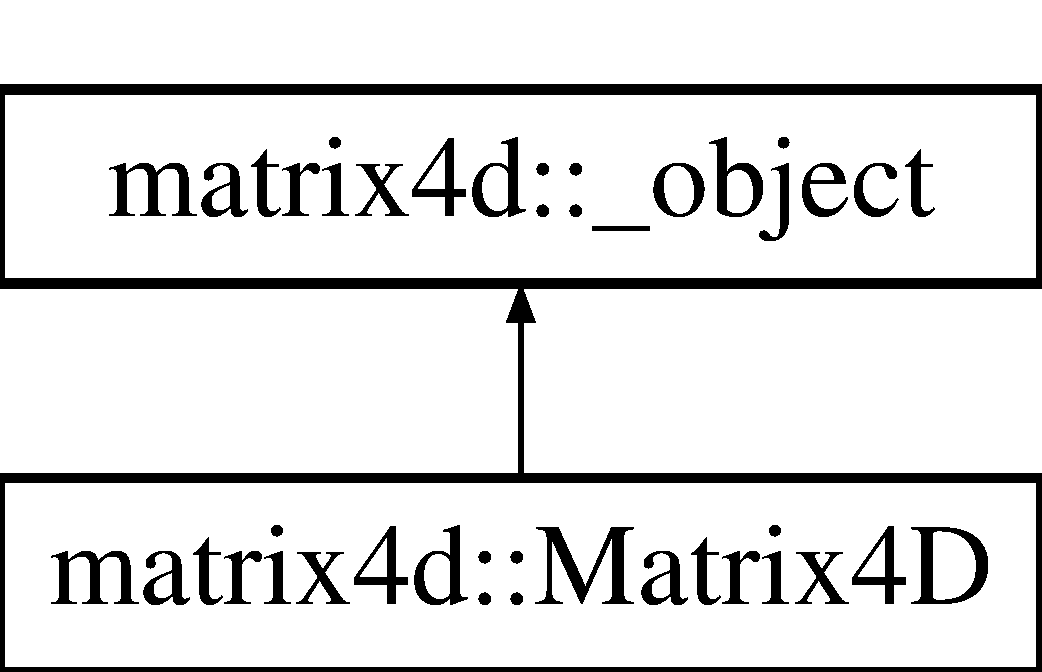
\includegraphics[height=2cm]{d8/d2d/classmatrix4d_1_1Matrix4D}
\end{center}
\end{figure}
\subsection*{Public Member Functions}
\begin{DoxyCompactItemize}
\item 
\hypertarget{classmatrix4d_1_1Matrix4D_aa8d774229c413810f9b45e3f9639e14a}{
def {\bfseries \_\-\_\-init\_\-\_\-}}
\label{d8/d2d/classmatrix4d_1_1Matrix4D_aa8d774229c413810f9b45e3f9639e14a}

\item 
\hypertarget{classmatrix4d_1_1Matrix4D_a6fafbf238ef7c28349d531f83fd8cf33}{
def {\bfseries GetVal}}
\label{d8/d2d/classmatrix4d_1_1Matrix4D_a6fafbf238ef7c28349d531f83fd8cf33}

\item 
\hypertarget{classmatrix4d_1_1Matrix4D_a2b5889d9f828b99718de148fca1be9f9}{
def {\bfseries SetVal}}
\label{d8/d2d/classmatrix4d_1_1Matrix4D_a2b5889d9f828b99718de148fca1be9f9}

\item 
\hypertarget{classmatrix4d_1_1Matrix4D_a3f9d959c9d4c8d5320747d7ee04c9fec}{
def {\bfseries GetNumDim1}}
\label{d8/d2d/classmatrix4d_1_1Matrix4D_a3f9d959c9d4c8d5320747d7ee04c9fec}

\item 
\hypertarget{classmatrix4d_1_1Matrix4D_a95aa43f9651d99efa51c414cbde29838}{
def {\bfseries GetNumDim2}}
\label{d8/d2d/classmatrix4d_1_1Matrix4D_a95aa43f9651d99efa51c414cbde29838}

\item 
\hypertarget{classmatrix4d_1_1Matrix4D_af60a9f91fa2c528f76bea466db63dd12}{
def {\bfseries GetNumDim3}}
\label{d8/d2d/classmatrix4d_1_1Matrix4D_af60a9f91fa2c528f76bea466db63dd12}

\item 
\hypertarget{classmatrix4d_1_1Matrix4D_ad1da489a0f84e1092e77a7586c03a062}{
def {\bfseries GetNumDim4}}
\label{d8/d2d/classmatrix4d_1_1Matrix4D_ad1da489a0f84e1092e77a7586c03a062}

\end{DoxyCompactItemize}
\subsection*{Public Attributes}
\begin{DoxyCompactItemize}
\item 
\hypertarget{classmatrix4d_1_1Matrix4D_a874437e826daf81e59bd8dad0fb64f00}{
{\bfseries this}}
\label{d8/d2d/classmatrix4d_1_1Matrix4D_a874437e826daf81e59bd8dad0fb64f00}

\end{DoxyCompactItemize}


The documentation for this class was generated from the following file:\begin{DoxyCompactItemize}
\item 
src/matrix4d.py\end{DoxyCompactItemize}

\hypertarget{classMaxSlope}{
\section{MaxSlope Class Reference}
\label{d0/d39/classMaxSlope}\index{MaxSlope@{MaxSlope}}
}
Inheritance diagram for MaxSlope::\begin{figure}[H]
\begin{center}
\leavevmode
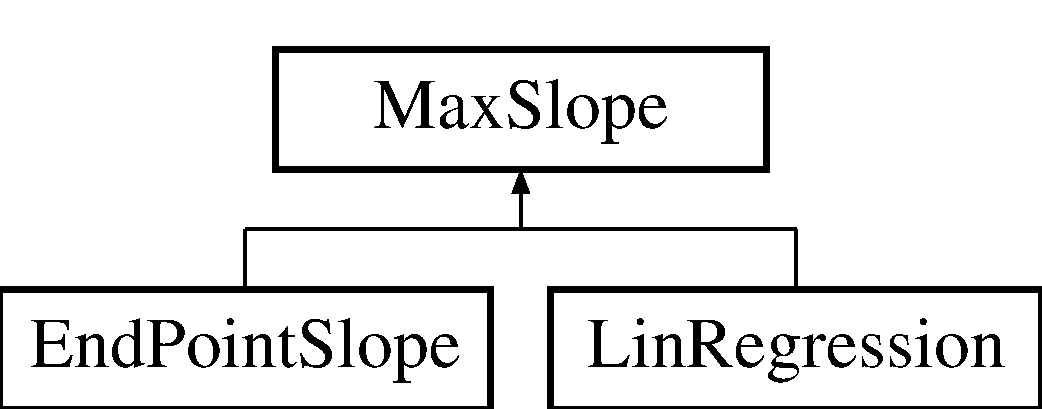
\includegraphics[height=2cm]{d0/d39/classMaxSlope}
\end{center}
\end{figure}
\subsection*{Public Member Functions}
\begin{DoxyCompactItemize}
\item 
\hypertarget{classMaxSlope_a494b1b1ae073d3b29fe7cdc023ce7861}{
virtual int \hyperlink{classMaxSlope_a494b1b1ae073d3b29fe7cdc023ce7861}{MostMonotonic} (int $\ast$monoAry, const int ncols, const int col)=0}
\label{d0/d39/classMaxSlope_a494b1b1ae073d3b29fe7cdc023ce7861}

\begin{DoxyCompactList}\small\item\em Virtual function to be inherited by each monotonicity checking algorithm to determine the most monotonic progress variable. \item\end{DoxyCompactList}\end{DoxyCompactItemize}


The documentation for this class was generated from the following file:\begin{DoxyCompactItemize}
\item 
src/maxslope.h\end{DoxyCompactItemize}

\hypertarget{classmaxslope_1_1MaxSlope}{
\section{maxslope::MaxSlope Class Reference}
\label{d8/deb/classmaxslope_1_1MaxSlope}\index{maxslope::MaxSlope@{maxslope::MaxSlope}}
}
Inheritance diagram for maxslope::MaxSlope::\begin{figure}[H]
\begin{center}
\leavevmode
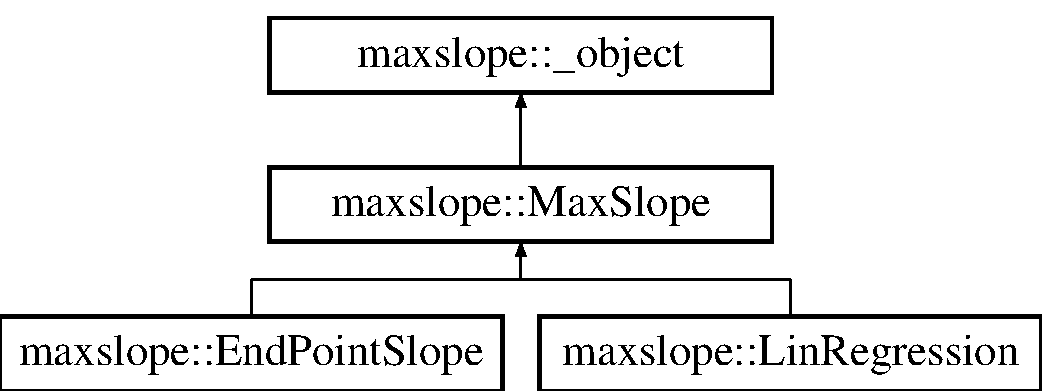
\includegraphics[height=3cm]{d8/deb/classmaxslope_1_1MaxSlope}
\end{center}
\end{figure}
\subsection*{Public Member Functions}
\begin{DoxyCompactItemize}
\item 
\hypertarget{classmaxslope_1_1MaxSlope_a362903e9e198c5d097c7c09ae6f74dd8}{
def {\bfseries \_\-\_\-init\_\-\_\-}}
\label{d8/deb/classmaxslope_1_1MaxSlope_a362903e9e198c5d097c7c09ae6f74dd8}

\item 
\hypertarget{classmaxslope_1_1MaxSlope_a6fda530ba01a2b4bc78f7c1ad841cabf}{
def {\bfseries MostMonotonic}}
\label{d8/deb/classmaxslope_1_1MaxSlope_a6fda530ba01a2b4bc78f7c1ad841cabf}

\end{DoxyCompactItemize}


The documentation for this class was generated from the following file:\begin{DoxyCompactItemize}
\item 
src/maxslope.py\end{DoxyCompactItemize}

\hypertarget{classmonocheck_1_1MonoCheck}{
\section{monocheck::MonoCheck Class Reference}
\label{d7/de1/classmonocheck_1_1MonoCheck}\index{monocheck::MonoCheck@{monocheck::MonoCheck}}
}
Inheritance diagram for monocheck::MonoCheck::\begin{figure}[H]
\begin{center}
\leavevmode
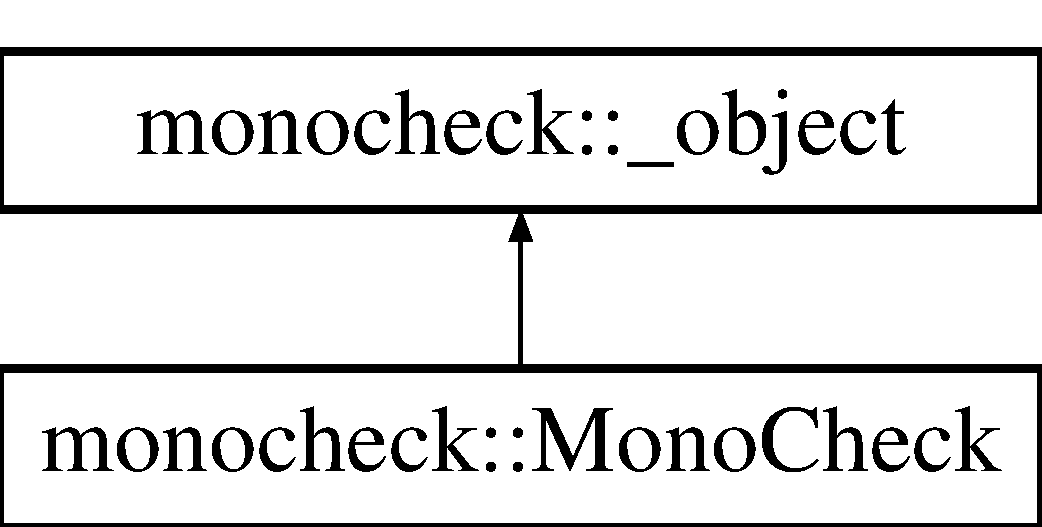
\includegraphics[height=2cm]{d7/de1/classmonocheck_1_1MonoCheck}
\end{center}
\end{figure}
\subsection*{Public Member Functions}
\begin{DoxyCompactItemize}
\item 
\hypertarget{classmonocheck_1_1MonoCheck_a69a5e0b89b39ff0c0caac2604605dddd}{
def {\bfseries \_\-\_\-init\_\-\_\-}}
\label{d7/de1/classmonocheck_1_1MonoCheck_a69a5e0b89b39ff0c0caac2604605dddd}

\item 
\hypertarget{classmonocheck_1_1MonoCheck_a9684b1459e63268cf3a3962e79827355}{
def {\bfseries CheckStrictMonoticity}}
\label{d7/de1/classmonocheck_1_1MonoCheck_a9684b1459e63268cf3a3962e79827355}

\end{DoxyCompactItemize}
\subsection*{Public Attributes}
\begin{DoxyCompactItemize}
\item 
\hypertarget{classmonocheck_1_1MonoCheck_a4e896031c1c1933907b882f4c4807cae}{
{\bfseries this}}
\label{d7/de1/classmonocheck_1_1MonoCheck_a4e896031c1c1933907b882f4c4807cae}

\end{DoxyCompactItemize}


The documentation for this class was generated from the following file:\begin{DoxyCompactItemize}
\item 
src/monocheck.py\end{DoxyCompactItemize}

\hypertarget{classMonoCheck}{
\section{MonoCheck Class Reference}
\label{d8/ddf/classMonoCheck}\index{MonoCheck@{MonoCheck}}
}
\subsection*{Public Member Functions}
\begin{DoxyCompactItemize}
\item 
\hyperlink{classMonoCheck_a4cee9c89dd8a6c19cd01d597343c4d99}{MonoCheck} (const \hyperlink{classMatrix}{Matrix} \&progVar)
\begin{DoxyCompactList}\small\item\em Constructor. \item\end{DoxyCompactList}\item 
\hypertarget{classMonoCheck_a97dc563e5cad68eafabd498d66e86590}{
\hyperlink{classMonoCheck_a97dc563e5cad68eafabd498d66e86590}{$\sim$MonoCheck} ()}
\label{d8/ddf/classMonoCheck_a97dc563e5cad68eafabd498d66e86590}

\begin{DoxyCompactList}\small\item\em Destructor. \item\end{DoxyCompactList}\item 
int \hyperlink{classMonoCheck_af34f3d72ec2d1575526d42bfe4cdfe7a}{CheckStrictMonoticity} (int $\ast$monoAry, const int ncols, int col)
\begin{DoxyCompactList}\small\item\em Method to check whether each progress variable is strictly monotonic. \item\end{DoxyCompactList}\end{DoxyCompactItemize}


\subsection{Constructor \& Destructor Documentation}
\hypertarget{classMonoCheck_a4cee9c89dd8a6c19cd01d597343c4d99}{
\index{MonoCheck@{MonoCheck}!MonoCheck@{MonoCheck}}
\index{MonoCheck@{MonoCheck}!MonoCheck@{MonoCheck}}
\subsubsection[{MonoCheck}]{\setlength{\rightskip}{0pt plus 5cm}MonoCheck::MonoCheck (const {\bf Matrix} \& {\em progVar})}}
\label{d8/ddf/classMonoCheck_a4cee9c89dd8a6c19cd01d597343c4d99}


Constructor. monocheck is a class which checks whether a specified progress variable is strictly increasing or strictly decreasing with respect to temperature (or another specified column). That is, C(T1)$<$C(T2) or C(T1)$>$C(T2) for T1$<$T2, where T1 and T2 are any two temperatures and C is the progress variable. 

\subsection{Member Function Documentation}
\hypertarget{classMonoCheck_af34f3d72ec2d1575526d42bfe4cdfe7a}{
\index{MonoCheck@{MonoCheck}!CheckStrictMonoticity@{CheckStrictMonoticity}}
\index{CheckStrictMonoticity@{CheckStrictMonoticity}!MonoCheck@{MonoCheck}}
\subsubsection[{CheckStrictMonoticity}]{\setlength{\rightskip}{0pt plus 5cm}int MonoCheck::CheckStrictMonoticity (int $\ast$ {\em monoAry}, \/  const int {\em ncols}, \/  int {\em col})}}
\label{d8/ddf/classMonoCheck_af34f3d72ec2d1575526d42bfe4cdfe7a}


Method to check whether each progress variable is strictly monotonic. CheckStrictMonoticity checks the monotonicity of each column (AKA progress variable \char`\"{}C\char`\"{}) in progVar with respect to column \char`\"{}col\char`\"{}. The output array monoAry must be of length ncols\_\-, where each cell holds a value of 3 if C is strictly increasing or strictly decreasing and 0 otherwise. 

The documentation for this class was generated from the following files:\begin{DoxyCompactItemize}
\item 
src/monocheck.h\item 
src/monocheck.cc\end{DoxyCompactItemize}

\hypertarget{classPDF}{
\section{PDF Class Reference}
\label{dc/d2d/classPDF}\index{PDF@{PDF}}
}
Inheritance diagram for PDF::\begin{figure}[H]
\begin{center}
\leavevmode
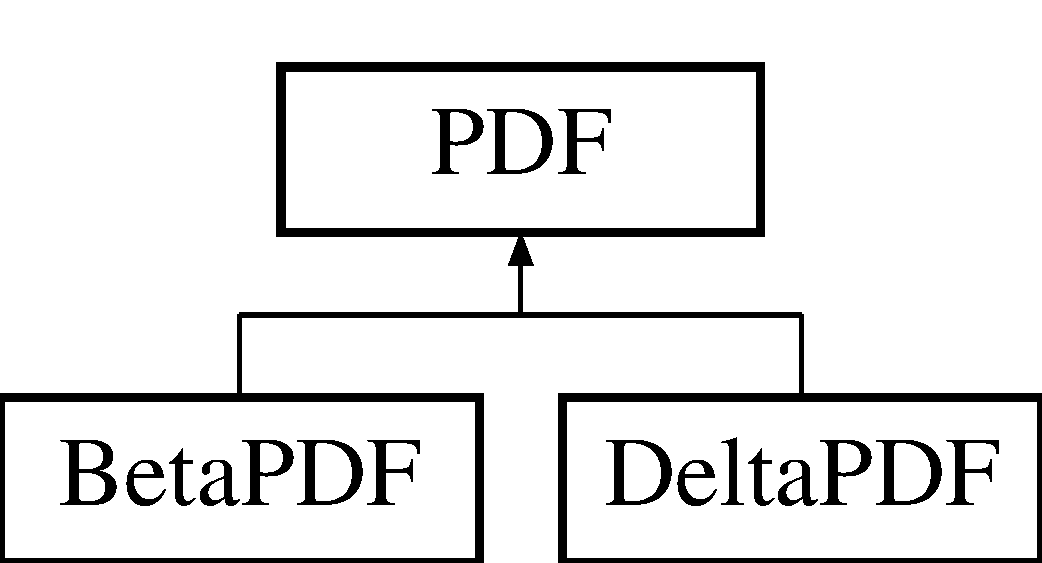
\includegraphics[height=2cm]{dc/d2d/classPDF}
\end{center}
\end{figure}
\subsection*{Public Member Functions}
\begin{DoxyCompactItemize}
\item 
\hypertarget{classPDF_aa1c76d504f181d271734bba54068c51b}{
virtual int {\bfseries pdfVal} (const double $\ast$Z, const int ZPoints, \hyperlink{classMatrix3D}{Matrix3D} $\ast$pdfValM)=0}
\label{dc/d2d/classPDF_aa1c76d504f181d271734bba54068c51b}

\end{DoxyCompactItemize}


The documentation for this class was generated from the following file:\begin{DoxyCompactItemize}
\item 
src/pdf.h\end{DoxyCompactItemize}

\hypertarget{classpdf_1_1PDF}{
\section{pdf::PDF Class Reference}
\label{dd/d66/classpdf_1_1PDF}\index{pdf::PDF@{pdf::PDF}}
}
Inheritance diagram for pdf::PDF::\begin{figure}[H]
\begin{center}
\leavevmode
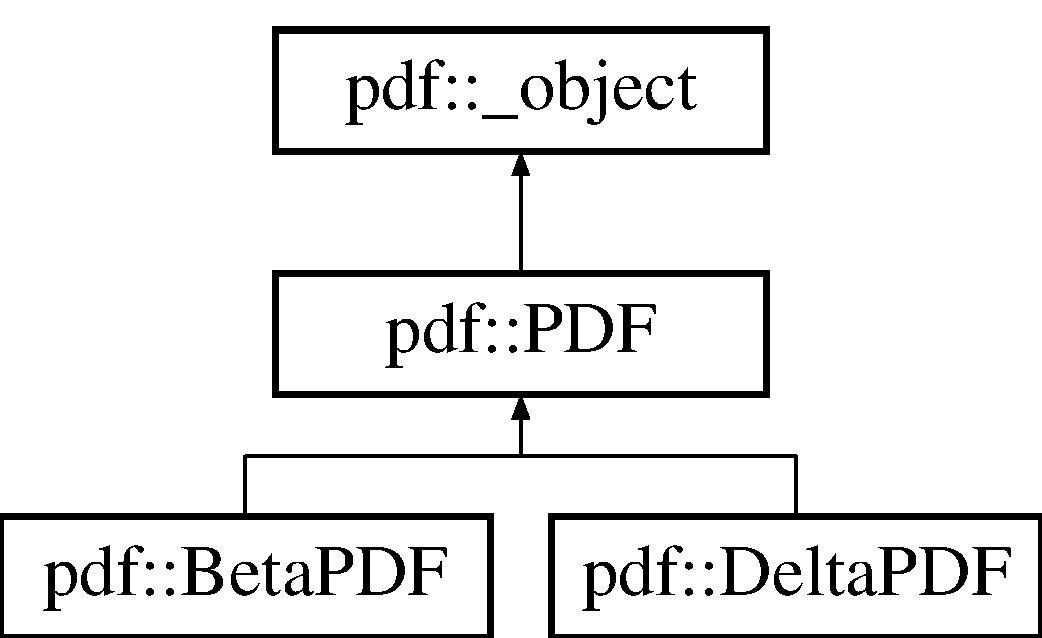
\includegraphics[height=3cm]{dd/d66/classpdf_1_1PDF}
\end{center}
\end{figure}
\subsection*{Public Member Functions}
\begin{DoxyCompactItemize}
\item 
\hypertarget{classpdf_1_1PDF_ad3afb94bbbcb72475c89d7bb3f946da2}{
def {\bfseries \_\-\_\-init\_\-\_\-}}
\label{dd/d66/classpdf_1_1PDF_ad3afb94bbbcb72475c89d7bb3f946da2}

\item 
\hypertarget{classpdf_1_1PDF_a44e17a10e5b431ab10ed1f5741d05e30}{
def {\bfseries pdfVal}}
\label{dd/d66/classpdf_1_1PDF_a44e17a10e5b431ab10ed1f5741d05e30}

\end{DoxyCompactItemize}


The documentation for this class was generated from the following file:\begin{DoxyCompactItemize}
\item 
src/pdf.py\end{DoxyCompactItemize}

\hypertarget{classiofuncs_1_1ProcFile}{
\section{iofuncs::ProcFile Class Reference}
\label{d3/d16/classiofuncs_1_1ProcFile}\index{iofuncs::ProcFile@{iofuncs::ProcFile}}
}
\subsection*{Public Member Functions}
\begin{DoxyCompactItemize}
\item 
def \hyperlink{classiofuncs_1_1ProcFile_aaf57101eb0b922217a240ca283fc5d9d}{\_\-\_\-init\_\-\_\-}
\begin{DoxyCompactList}\small\item\em The Constructor. \item\end{DoxyCompactList}\item 
def \hyperlink{classiofuncs_1_1ProcFile_a88f142260af3fd70b1b8613da471f858}{gettitles}
\begin{DoxyCompactList}\small\item\em Function that returns a vector containing the column headers in the 2nd row of the data file. \item\end{DoxyCompactList}\item 
def \hyperlink{classiofuncs_1_1ProcFile_ae7f8d6213747a8d1e41b771ec71cd2be}{interpolate}
\begin{DoxyCompactList}\small\item\em Interpolate function extracts/interpolates a row of data in the data file at the specified value in the first column. \item\end{DoxyCompactList}\end{DoxyCompactItemize}


\subsection{Detailed Description}
\begin{DoxyVerb}Class for processing .kg datafiles, including extracting column headers and interpolating a row of data.\end{DoxyVerb}
 

\subsection{Member Function Documentation}
\hypertarget{classiofuncs_1_1ProcFile_aaf57101eb0b922217a240ca283fc5d9d}{
\index{iofuncs::ProcFile@{iofuncs::ProcFile}!\_\-\_\-init\_\-\_\-@{\_\-\_\-init\_\-\_\-}}
\index{\_\-\_\-init\_\-\_\-@{\_\-\_\-init\_\-\_\-}!iofuncs::ProcFile@{iofuncs::ProcFile}}
\subsubsection[{\_\-\_\-init\_\-\_\-}]{\setlength{\rightskip}{0pt plus 5cm}def iofuncs::ProcFile::\_\-\_\-init\_\-\_\- ( {\em self}, \/   {\em sfile})}}
\label{d3/d16/classiofuncs_1_1ProcFile_aaf57101eb0b922217a240ca283fc5d9d}


The Constructor. SFILE: a string contiaining the name of the data file to be processed or path to that file \hypertarget{classiofuncs_1_1ProcFile_a88f142260af3fd70b1b8613da471f858}{
\index{iofuncs::ProcFile@{iofuncs::ProcFile}!gettitles@{gettitles}}
\index{gettitles@{gettitles}!iofuncs::ProcFile@{iofuncs::ProcFile}}
\subsubsection[{gettitles}]{\setlength{\rightskip}{0pt plus 5cm}def iofuncs::ProcFile::gettitles ( {\em self})}}
\label{d3/d16/classiofuncs_1_1ProcFile_a88f142260af3fd70b1b8613da471f858}


Function that returns a vector containing the column headers in the 2nd row of the data file. Ignores 1st row, returns contents of 2nd row as elements of a vector (assuming datafile is tab delimited). \hypertarget{classiofuncs_1_1ProcFile_ae7f8d6213747a8d1e41b771ec71cd2be}{
\index{iofuncs::ProcFile@{iofuncs::ProcFile}!interpolate@{interpolate}}
\index{interpolate@{interpolate}!iofuncs::ProcFile@{iofuncs::ProcFile}}
\subsubsection[{interpolate}]{\setlength{\rightskip}{0pt plus 5cm}def iofuncs::ProcFile::interpolate ( {\em self}, \/   {\em inputvars}, \/   {\em locs}, \/   {\em datavec}, \/   {\em interpval} = {\ttfamily 0.27}, \/   {\em interpmethod} = {\ttfamily 'linear'})}}
\label{d3/d16/classiofuncs_1_1ProcFile_ae7f8d6213747a8d1e41b771ec71cd2be}


Interpolate function extracts/interpolates a row of data in the data file at the specified value in the first column. Read the columns of the data file with headers matching the strings in the INPUTVARS vector.

Write the column numbers corresponding to these column headers into LOCS vector.

Interpolate to find values of each column corresponding to INTERPVAL in the 1st column, using interpolation method specified by the INTERPMETHOD string.

Write interpolated values to DATAVEC. 

The documentation for this class was generated from the following file:\begin{DoxyCompactItemize}
\item 
python/iofuncs.py\end{DoxyCompactItemize}

\hypertarget{classSequenceGen}{
\section{SequenceGen Class Reference}
\label{d4/d99/classSequenceGen}\index{SequenceGen@{SequenceGen}}
}


Sequence generator for the standard sorting algorithm.  
\subsection*{Public Member Functions}
\begin{DoxyCompactItemize}
\item 
\hypertarget{classSequenceGen_a4d1ef90f7ec766284371caf9e6c4f791}{
{\bfseries SequenceGen} (int start=0)}
\label{d4/d99/classSequenceGen_a4d1ef90f7ec766284371caf9e6c4f791}

\item 
\hypertarget{classSequenceGen_af63e6e7ae3a2fdcb86a6ed263f953c84}{
int {\bfseries operator()} ()}
\label{d4/d99/classSequenceGen_af63e6e7ae3a2fdcb86a6ed263f953c84}

\end{DoxyCompactItemize}


\subsection{Detailed Description}
Sequence generator for the standard sorting algorithm. 

The documentation for this class was generated from the following file:\begin{DoxyCompactItemize}
\item 
src/standardsort.cc\end{DoxyCompactItemize}

\hypertarget{classSimpleLNM}{
\section{SimpleLNM Class Reference}
\label{d8/dfe/classSimpleLNM}\index{SimpleLNM@{SimpleLNM}}
}
Inheritance diagram for SimpleLNM::\begin{figure}[H]
\begin{center}
\leavevmode
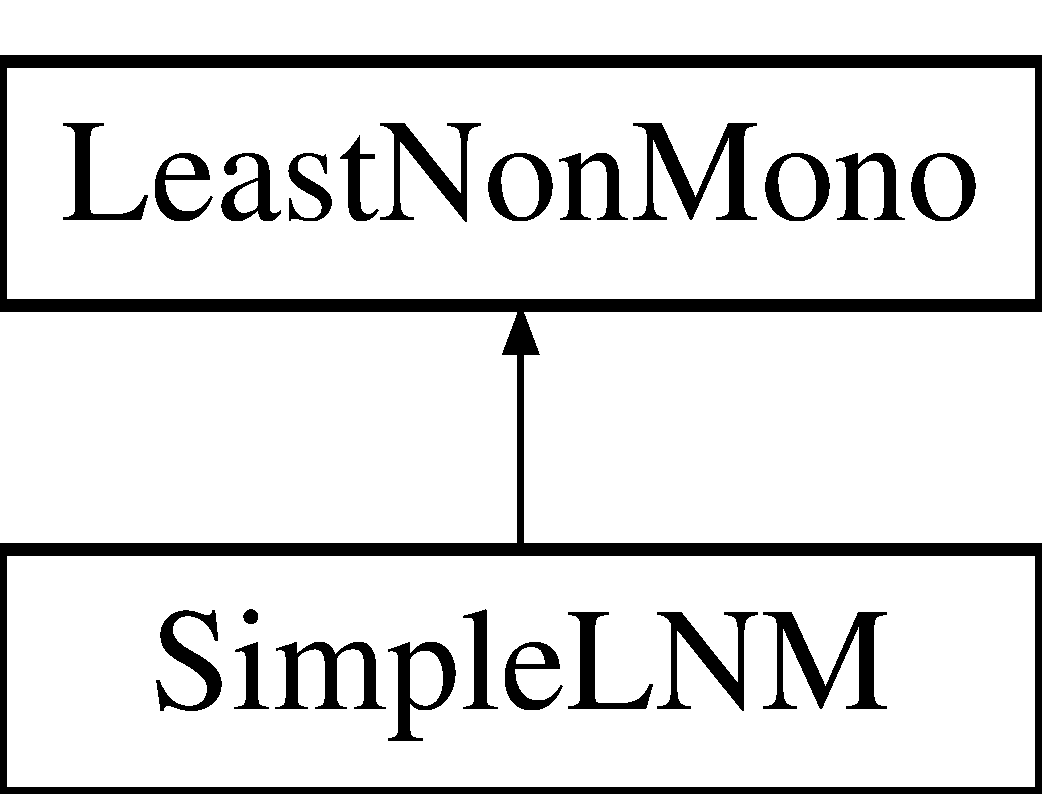
\includegraphics[height=2cm]{d8/dfe/classSimpleLNM}
\end{center}
\end{figure}
\subsection*{Public Member Functions}
\begin{DoxyCompactItemize}
\item 
\hyperlink{classSimpleLNM_a45bd676f6bb504baf1b46ddcbf2f8fb8}{SimpleLNM} (const \hyperlink{classMatrix}{Matrix} \&progVar)
\begin{DoxyCompactList}\small\item\em Constructor. \item\end{DoxyCompactList}\item 
\hypertarget{classSimpleLNM_a89cbe5270c4846ebba8ab1660149112f}{
\hyperlink{classSimpleLNM_a89cbe5270c4846ebba8ab1660149112f}{$\sim$SimpleLNM} ()}
\label{d8/dfe/classSimpleLNM_a89cbe5270c4846ebba8ab1660149112f}

\begin{DoxyCompactList}\small\item\em Destructor. \item\end{DoxyCompactList}\item 
int \hyperlink{classSimpleLNM_a9d296839ca84467c0f6241b1393bd6d5}{LeastNonMonotonic} (int $\ast$monoAry, const int ncols, const int col)
\begin{DoxyCompactList}\small\item\em Method to find the least non monotonic progress variable. \item\end{DoxyCompactList}\end{DoxyCompactItemize}


\subsection{Constructor \& Destructor Documentation}
\hypertarget{classSimpleLNM_a45bd676f6bb504baf1b46ddcbf2f8fb8}{
\index{SimpleLNM@{SimpleLNM}!SimpleLNM@{SimpleLNM}}
\index{SimpleLNM@{SimpleLNM}!SimpleLNM@{SimpleLNM}}
\subsubsection[{SimpleLNM}]{\setlength{\rightskip}{0pt plus 5cm}SimpleLNM::SimpleLNM (const {\bf Matrix} \& {\em progVar})}}
\label{d8/dfe/classSimpleLNM_a45bd676f6bb504baf1b46ddcbf2f8fb8}


Constructor. \hyperlink{classSimpleLNM}{SimpleLNM} is a class that determines the least non-\/monotonic progress variable with respect to temperature (or another specified column). It determines the percentage which the progress variable is strictly increasing and the percentage which the progress variable is strictly decreasing. The larger percentage not only determines whether the progress variable is increasing or decreasing, but will also be compared with the percentages of other progress variables. The progress variable with the largest percentage of increasing or decreasing values is the least non-\/monotonic progress variable.

If two or more progress variables share the highest percentage, then the progress variable with the greatest magnitude slope (by endpoints) is selected. Progress variables with neither increasing nor decreasing data are considered strongly non-\/monotonic. 

\subsection{Member Function Documentation}
\hypertarget{classSimpleLNM_a9d296839ca84467c0f6241b1393bd6d5}{
\index{SimpleLNM@{SimpleLNM}!LeastNonMonotonic@{LeastNonMonotonic}}
\index{LeastNonMonotonic@{LeastNonMonotonic}!SimpleLNM@{SimpleLNM}}
\subsubsection[{LeastNonMonotonic}]{\setlength{\rightskip}{0pt plus 5cm}int SimpleLNM::LeastNonMonotonic (int $\ast$ {\em monoAry}, \/  const int {\em ncols}, \/  const int {\em col})\hspace{0.3cm}{\ttfamily  \mbox{[}virtual\mbox{]}}}}
\label{d8/dfe/classSimpleLNM_a9d296839ca84467c0f6241b1393bd6d5}


Method to find the least non monotonic progress variable. LeastNonMonotonic calculates how much each progress variable is strictly increasing and strictly decreasing. The input array monoAry will initially be filled with 0s since all progress variables are non-\/monotonic. This method will select the least non-\/monotonic and change its value in monoAry to 1. col is the reference column.

\begin{DoxyVerb}
INPUTS: 

int *monoAry      array containing integer flags that denote the monotonicity of candidate slope variables

const int ncols   number of columns of monoAry

const int col     the reference column

OUTPUT:

int               flag specifying whether or not the function succeeded 
                   = 0: success
		  != 0: something went wrong

\end{DoxyVerb}
 

Implements \hyperlink{classLeastNonMono}{LeastNonMono}.

The documentation for this class was generated from the following files:\begin{DoxyCompactItemize}
\item 
src/simplelnm.h\item 
src/simplelnm.cc\end{DoxyCompactItemize}

\hypertarget{classleastnonmono_1_1SimpleLNM}{
\section{leastnonmono::SimpleLNM Class Reference}
\label{d8/df0/classleastnonmono_1_1SimpleLNM}\index{leastnonmono::SimpleLNM@{leastnonmono::SimpleLNM}}
}
Inheritance diagram for leastnonmono::SimpleLNM::\begin{figure}[H]
\begin{center}
\leavevmode
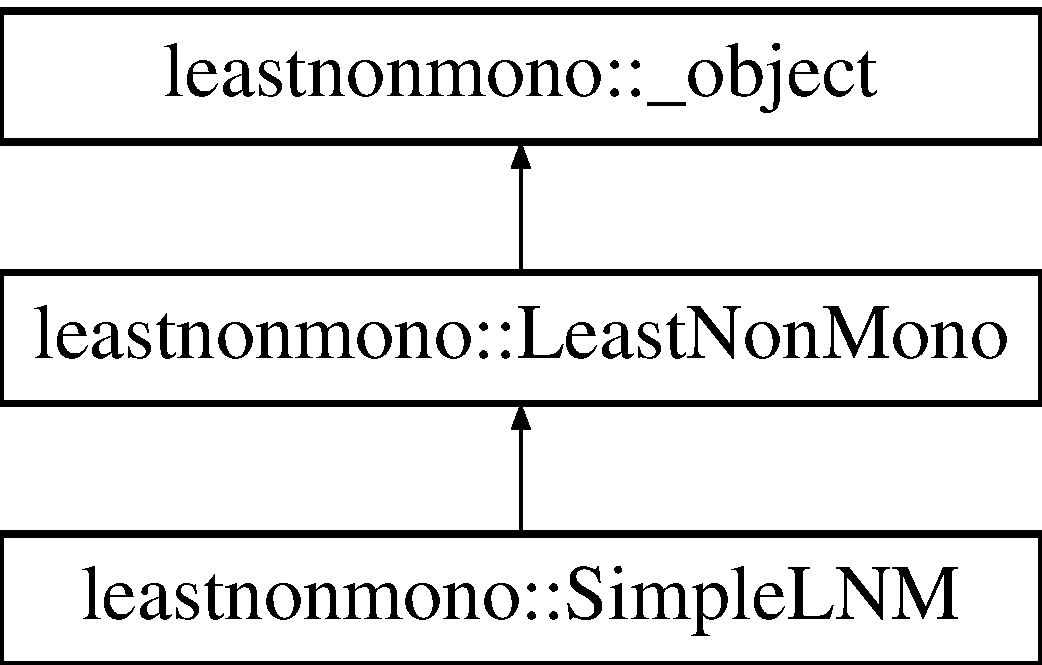
\includegraphics[height=3cm]{d8/df0/classleastnonmono_1_1SimpleLNM}
\end{center}
\end{figure}
\subsection*{Public Member Functions}
\begin{DoxyCompactItemize}
\item 
\hypertarget{classleastnonmono_1_1SimpleLNM_a60b4300be3d34df4505fa4a58eb214dd}{
def {\bfseries \_\-\_\-init\_\-\_\-}}
\label{d8/df0/classleastnonmono_1_1SimpleLNM_a60b4300be3d34df4505fa4a58eb214dd}

\item 
\hypertarget{classleastnonmono_1_1SimpleLNM_ac5c0bed3e296b52b508ad9f45860ac75}{
def {\bfseries LeastNonMonotonic}}
\label{d8/df0/classleastnonmono_1_1SimpleLNM_ac5c0bed3e296b52b508ad9f45860ac75}

\end{DoxyCompactItemize}
\subsection*{Public Attributes}
\begin{DoxyCompactItemize}
\item 
\hypertarget{classleastnonmono_1_1SimpleLNM_a0e7014df02df6a20c4a5d1a78e574303}{
{\bfseries this}}
\label{d8/df0/classleastnonmono_1_1SimpleLNM_a0e7014df02df6a20c4a5d1a78e574303}

\end{DoxyCompactItemize}


The documentation for this class was generated from the following file:\begin{DoxyCompactItemize}
\item 
src/leastnonmono.py\end{DoxyCompactItemize}

\hypertarget{classSimpson}{
\section{Simpson Class Reference}
\label{d7/d99/classSimpson}\index{Simpson@{Simpson}}
}


Calculates integral using Simpson's rule.  


{\ttfamily \#include $<$simpson.h$>$}Inheritance diagram for Simpson::\begin{figure}[H]
\begin{center}
\leavevmode
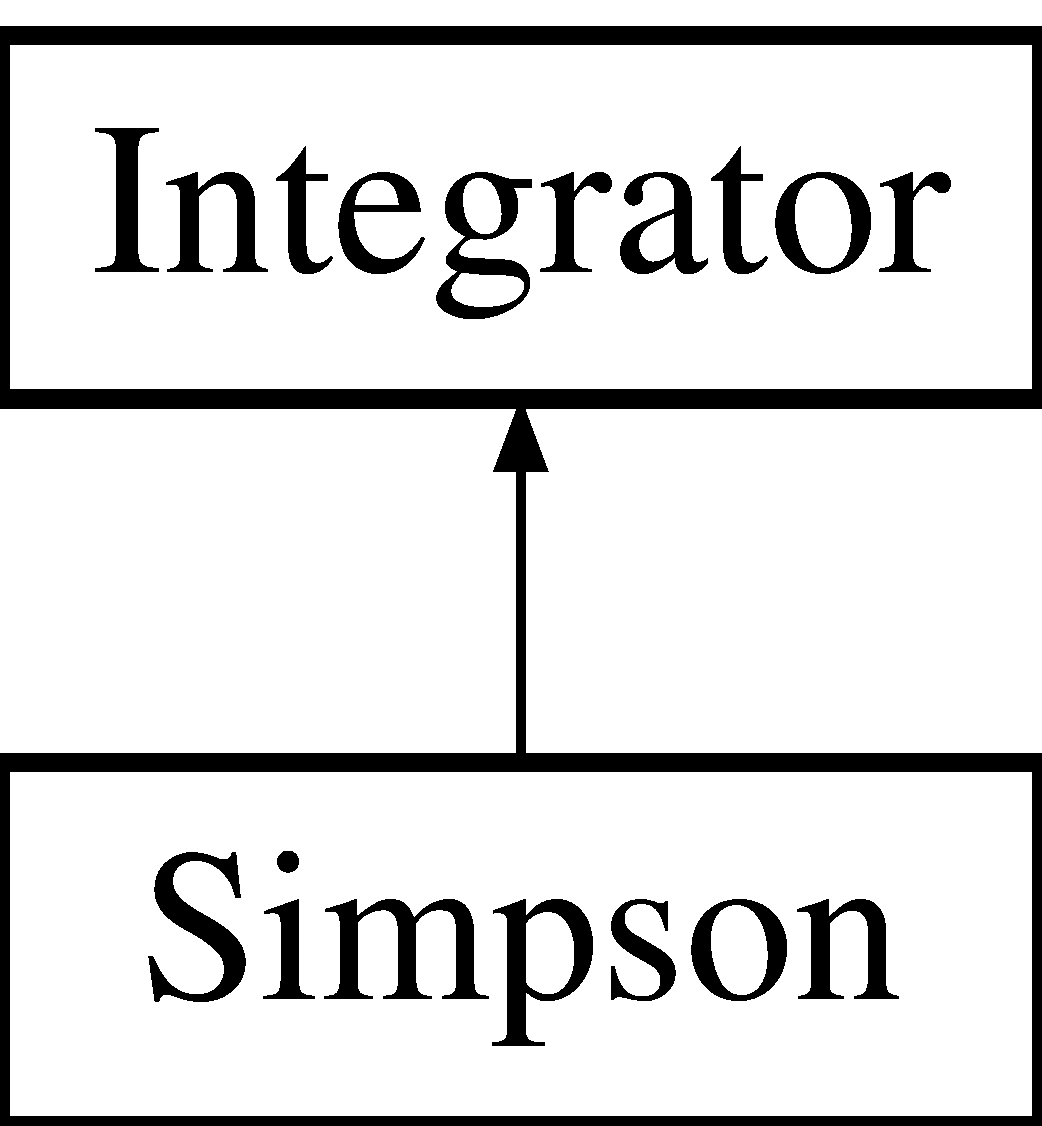
\includegraphics[height=2cm]{d7/d99/classSimpson}
\end{center}
\end{figure}
\subsection*{Public Member Functions}
\begin{DoxyCompactItemize}
\item 
\hypertarget{classSimpson_a67630263e3dafdfaa033f566324b4799}{
\hyperlink{classSimpson_a67630263e3dafdfaa033f566324b4799}{Simpson} ()}
\label{d7/d99/classSimpson_a67630263e3dafdfaa033f566324b4799}

\begin{DoxyCompactList}\small\item\em Constructor. \item\end{DoxyCompactList}\item 
\hypertarget{classSimpson_a92c73e59a11fdf7a156b3682676de6b8}{
\hyperlink{classSimpson_a92c73e59a11fdf7a156b3682676de6b8}{$\sim$Simpson} ()}
\label{d7/d99/classSimpson_a92c73e59a11fdf7a156b3682676de6b8}

\begin{DoxyCompactList}\small\item\em Destructor. \item\end{DoxyCompactList}\item 
double \hyperlink{classSimpson_ab90da2fb197efe2f4a669bf5029a16f4}{integrate} (const double $\ast$integrand, const double $\ast$Z, const int ZPoints)
\begin{DoxyCompactList}\small\item\em Main function that integrates a given data set using Simpson's Rule. \item\end{DoxyCompactList}\end{DoxyCompactItemize}


\subsection{Detailed Description}
Calculates integral using Simpson's rule. \hyperlink{classSimpson}{Simpson} takes in an array (the integrand) and returns the integral of that array using Simpson's rule. 

\subsection{Member Function Documentation}
\hypertarget{classSimpson_ab90da2fb197efe2f4a669bf5029a16f4}{
\index{Simpson@{Simpson}!integrate@{integrate}}
\index{integrate@{integrate}!Simpson@{Simpson}}
\subsubsection[{integrate}]{\setlength{\rightskip}{0pt plus 5cm}double Simpson::integrate (const double $\ast$ {\em integrand}, \/  const double $\ast$ {\em Z}, \/  const int {\em ZPoints})\hspace{0.3cm}{\ttfamily  \mbox{[}virtual\mbox{]}}}}
\label{d7/d99/classSimpson_ab90da2fb197efe2f4a669bf5029a16f4}


Main function that integrates a given data set using Simpson's Rule. Simpson's rule is applied to integrate a given integrand over a given double array, Z.

\begin{DoxyVerb}
  INPUTS: 

  const double *integrand           array that contains function values to be integrated

  const double *Z                   array that contains the mixture fraction values which the integrand will be integrated over

  const int ZPoints                 number of values, size of the integrand and Z arrays


  OUTPUT:

  double                            result of the integration

  \end{DoxyVerb}
 

Implements \hyperlink{classIntegrator_a89fbef2f7923ce4e2c979b2ff1d1f4ac}{Integrator}.

The documentation for this class was generated from the following files:\begin{DoxyCompactItemize}
\item 
src/simpson.h\item 
src/simpson.cc\end{DoxyCompactItemize}

\hypertarget{classintegrator_1_1Simpson}{
\section{integrator::Simpson Class Reference}
\label{d0/d4a/classintegrator_1_1Simpson}\index{integrator::Simpson@{integrator::Simpson}}
}
Inheritance diagram for integrator::Simpson::\begin{figure}[H]
\begin{center}
\leavevmode
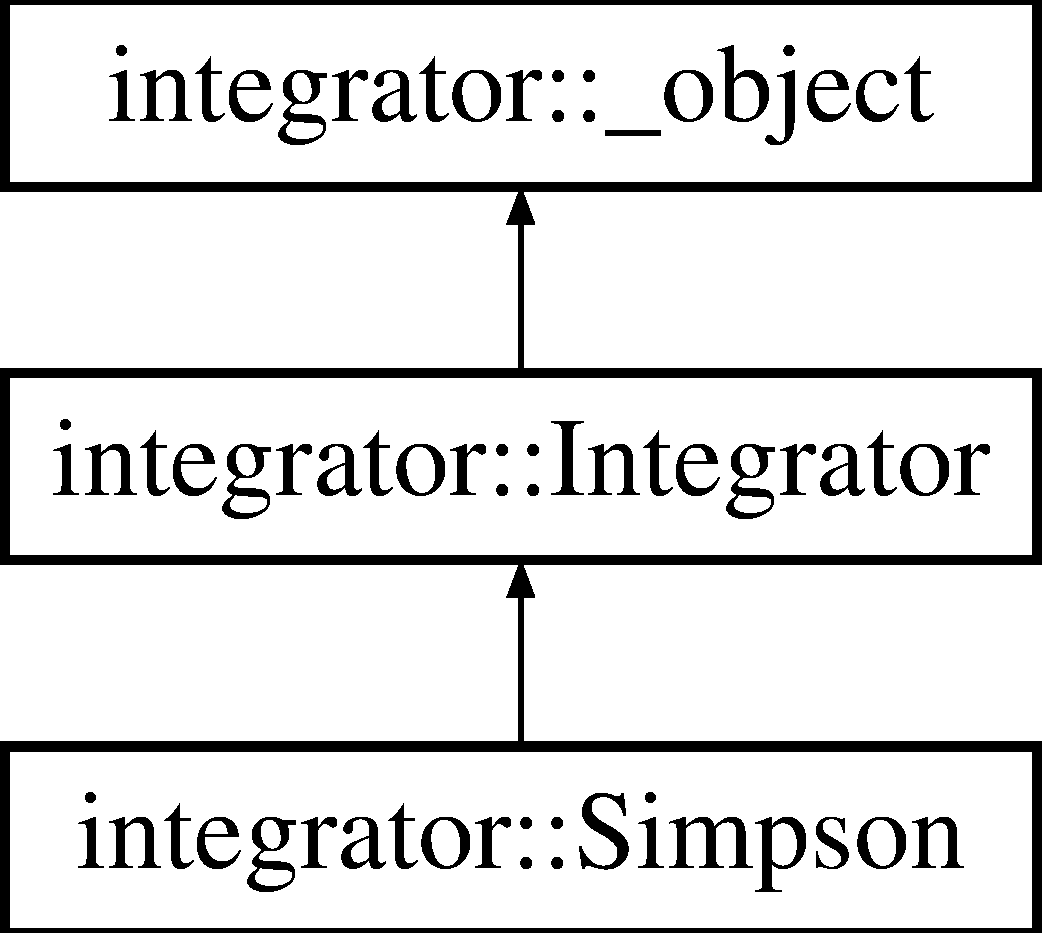
\includegraphics[height=3cm]{d0/d4a/classintegrator_1_1Simpson}
\end{center}
\end{figure}
\subsection*{Public Member Functions}
\begin{DoxyCompactItemize}
\item 
\hypertarget{classintegrator_1_1Simpson_a17d1008804885fc6afe3790365ffa9e7}{
def {\bfseries \_\-\_\-init\_\-\_\-}}
\label{d0/d4a/classintegrator_1_1Simpson_a17d1008804885fc6afe3790365ffa9e7}

\item 
\hypertarget{classintegrator_1_1Simpson_a8af6b307046196ddefc88456f2341b16}{
def {\bfseries integrate}}
\label{d0/d4a/classintegrator_1_1Simpson_a8af6b307046196ddefc88456f2341b16}

\end{DoxyCompactItemize}
\subsection*{Public Attributes}
\begin{DoxyCompactItemize}
\item 
\hypertarget{classintegrator_1_1Simpson_a891a4cebf60a703f96f1bbd8d1add1e2}{
{\bfseries this}}
\label{d0/d4a/classintegrator_1_1Simpson_a891a4cebf60a703f96f1bbd8d1add1e2}

\end{DoxyCompactItemize}


The documentation for this class was generated from the following file:\begin{DoxyCompactItemize}
\item 
src/integrator.py\end{DoxyCompactItemize}

\hypertarget{classsorting}{
\section{sorting Class Reference}
\label{df/d42/classsorting}\index{sorting@{sorting}}
}
Inheritance diagram for sorting::\begin{figure}[H]
\begin{center}
\leavevmode
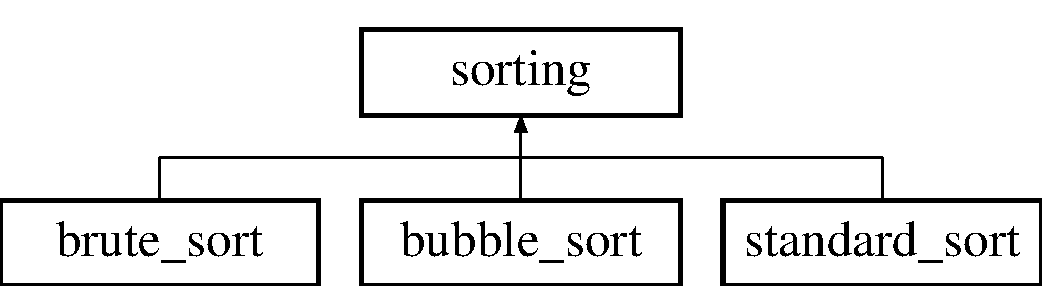
\includegraphics[height=2cm]{df/d42/classsorting}
\end{center}
\end{figure}
\subsection*{Public Member Functions}
\begin{DoxyCompactItemize}
\item 
\hypertarget{classsorting_a94c4b729732743299f3dcd2505312381}{
virtual int \hyperlink{classsorting_a94c4b729732743299f3dcd2505312381}{sort\_\-data} ()=0}
\label{df/d42/classsorting_a94c4b729732743299f3dcd2505312381}

\begin{DoxyCompactList}\small\item\em Virtual function to be inherited by each \hyperlink{classsorting}{sorting} algorithm to sort the give data. \item\end{DoxyCompactList}\item 
\hypertarget{classsorting_aee6e7f2f0ea31873c500e0692e4fc00c}{
virtual void \hyperlink{classsorting_aee6e7f2f0ea31873c500e0692e4fc00c}{SetRefColNum} (int num)}
\label{df/d42/classsorting_aee6e7f2f0ea31873c500e0692e4fc00c}

\begin{DoxyCompactList}\small\item\em Setting the reference column according to which the data will be sorted. \item\end{DoxyCompactList}\end{DoxyCompactItemize}


The documentation for this class was generated from the following file:\begin{DoxyCompactItemize}
\item 
src/sorting.h\end{DoxyCompactItemize}

\hypertarget{classsorting_1_1sorting}{
\section{sorting::sorting Class Reference}
\label{d8/d91/classsorting_1_1sorting}\index{sorting::sorting@{sorting::sorting}}
}
Inheritance diagram for sorting::sorting::\begin{figure}[H]
\begin{center}
\leavevmode
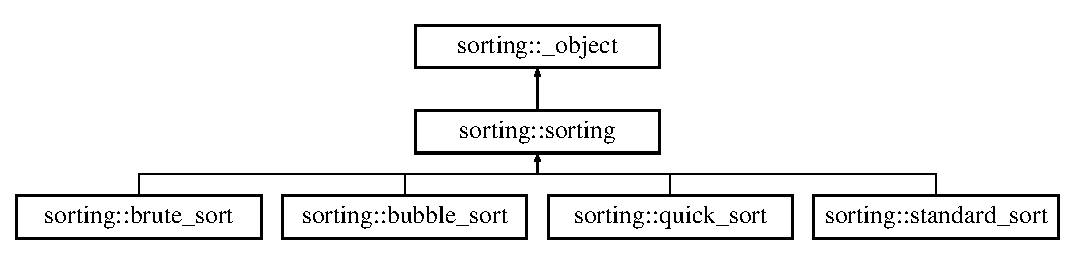
\includegraphics[height=3cm]{d8/d91/classsorting_1_1sorting}
\end{center}
\end{figure}
\subsection*{Public Member Functions}
\begin{DoxyCompactItemize}
\item 
\hypertarget{classsorting_1_1sorting_a487be5019cf669d6d4930ad1a7b4d31e}{
def {\bfseries \_\-\_\-init\_\-\_\-}}
\label{d8/d91/classsorting_1_1sorting_a487be5019cf669d6d4930ad1a7b4d31e}

\item 
\hypertarget{classsorting_1_1sorting_a2c7684816ed4940fb02326561d442cb1}{
def {\bfseries sort\_\-data}}
\label{d8/d91/classsorting_1_1sorting_a2c7684816ed4940fb02326561d442cb1}

\item 
\hypertarget{classsorting_1_1sorting_a4cafa3bef073b1b54155bda4e1f8e216}{
def {\bfseries SetRefColNum}}
\label{d8/d91/classsorting_1_1sorting_a4cafa3bef073b1b54155bda4e1f8e216}

\end{DoxyCompactItemize}


The documentation for this class was generated from the following file:\begin{DoxyCompactItemize}
\item 
src/sorting.py\end{DoxyCompactItemize}

\hypertarget{classstandard__sort}{
\section{standard\_\-sort Class Reference}
\label{d4/dec/classstandard__sort}\index{standard\_\-sort@{standard\_\-sort}}
}
Inheritance diagram for standard\_\-sort::\begin{figure}[H]
\begin{center}
\leavevmode
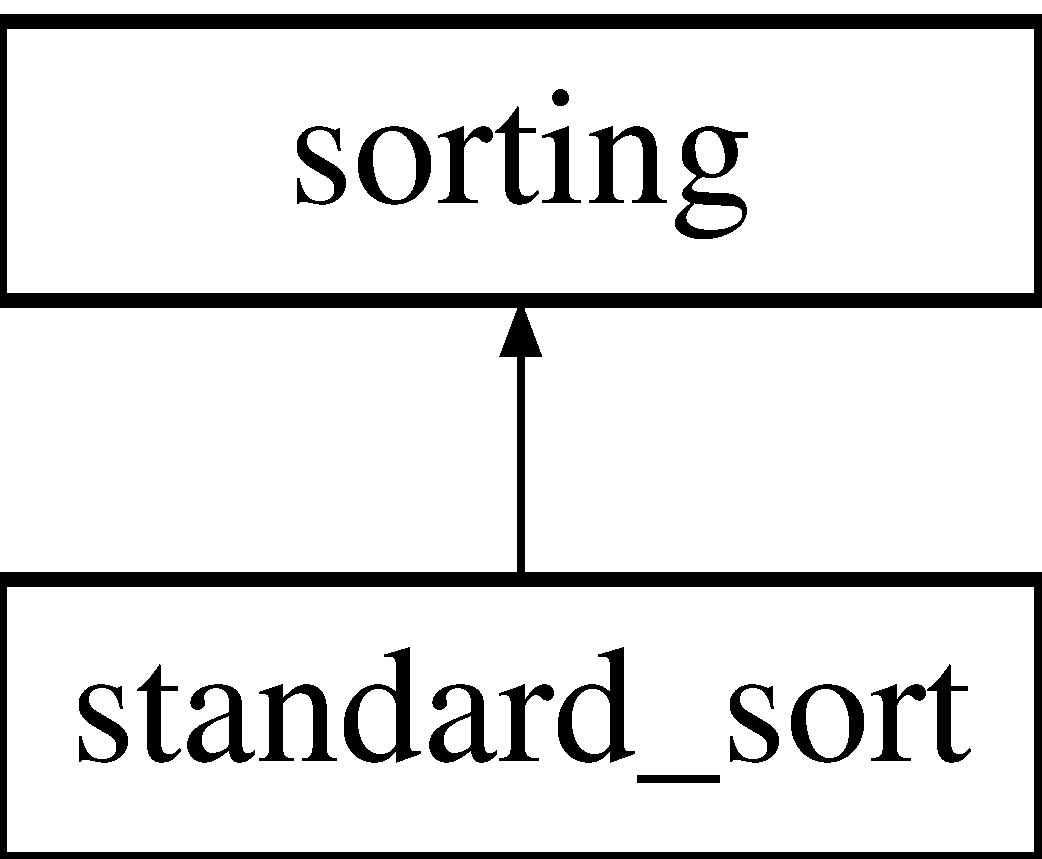
\includegraphics[height=2cm]{d4/dec/classstandard__sort}
\end{center}
\end{figure}
\subsection*{Public Member Functions}
\begin{DoxyCompactItemize}
\item 
\hypertarget{classstandard__sort_a70a7e1ba1cae2d294b252f6182f81436}{
\hyperlink{classstandard__sort_a70a7e1ba1cae2d294b252f6182f81436}{standard\_\-sort} (\hyperlink{classMatrix}{Matrix} $\ast$data)}
\label{d4/dec/classstandard__sort_a70a7e1ba1cae2d294b252f6182f81436}

\begin{DoxyCompactList}\small\item\em Constructor. \item\end{DoxyCompactList}\item 
\hypertarget{classstandard__sort_af40099379c12e092519a20afbad5c6b9}{
\hyperlink{classstandard__sort_af40099379c12e092519a20afbad5c6b9}{$\sim$standard\_\-sort} ()}
\label{d4/dec/classstandard__sort_af40099379c12e092519a20afbad5c6b9}

\begin{DoxyCompactList}\small\item\em Destructor. \item\end{DoxyCompactList}\item 
int \hyperlink{classstandard__sort_a34a0d914ebac6e328dfe371a1e1a8afb}{sort\_\-data} ()
\begin{DoxyCompactList}\small\item\em Main function that sorts the given data. \item\end{DoxyCompactList}\item 
\hypertarget{classstandard__sort_a5bf11721c6c6147440c68409b830a31a}{
void \hyperlink{classstandard__sort_a5bf11721c6c6147440c68409b830a31a}{SetRefColNum} (int num)}
\label{d4/dec/classstandard__sort_a5bf11721c6c6147440c68409b830a31a}

\begin{DoxyCompactList}\small\item\em Set the reference column number. \item\end{DoxyCompactList}\end{DoxyCompactItemize}


\subsection{Member Function Documentation}
\hypertarget{classstandard__sort_a34a0d914ebac6e328dfe371a1e1a8afb}{
\index{standard\_\-sort@{standard\_\-sort}!sort\_\-data@{sort\_\-data}}
\index{sort\_\-data@{sort\_\-data}!standard_sort@{standard\_\-sort}}
\subsubsection[{sort\_\-data}]{\setlength{\rightskip}{0pt plus 5cm}int standard\_\-sort::sort\_\-data ()\hspace{0.3cm}{\ttfamily  \mbox{[}virtual\mbox{]}}}}
\label{d4/dec/classstandard__sort_a34a0d914ebac6e328dfe371a1e1a8afb}


Main function that sorts the given data. The algorithm sends the reference column to the standard \hyperlink{classsorting}{sorting} operator that is embedded into the C++ standard library 

Implements \hyperlink{classsorting_a94c4b729732743299f3dcd2505312381}{sorting}.

The documentation for this class was generated from the following files:\begin{DoxyCompactItemize}
\item 
src/standard\_\-sort.h\item 
src/standard\_\-sort.cc\end{DoxyCompactItemize}

\hypertarget{classsorting_1_1standard__sort}{
\section{sorting::standard\_\-sort Class Reference}
\label{d4/d39/classsorting_1_1standard__sort}\index{sorting::standard\_\-sort@{sorting::standard\_\-sort}}
}
Inheritance diagram for sorting::standard\_\-sort::\begin{figure}[H]
\begin{center}
\leavevmode
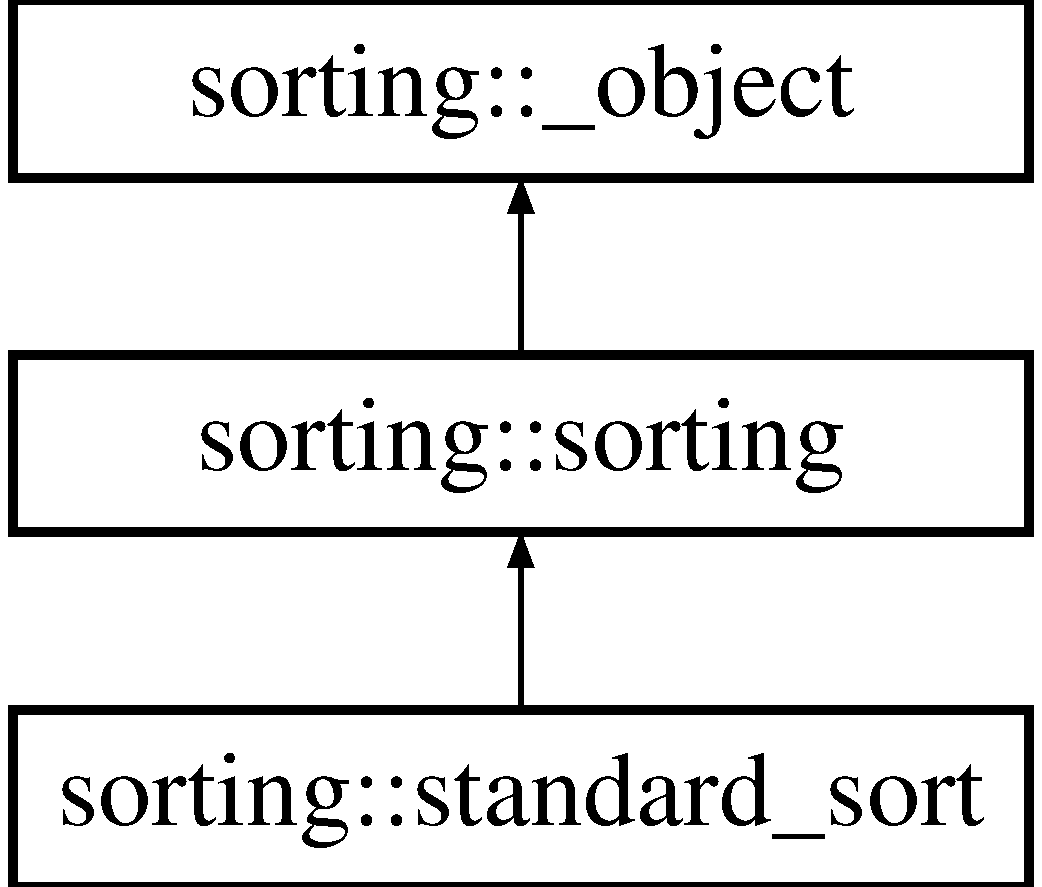
\includegraphics[height=3cm]{d4/d39/classsorting_1_1standard__sort}
\end{center}
\end{figure}
\subsection*{Public Member Functions}
\begin{DoxyCompactItemize}
\item 
\hypertarget{classsorting_1_1standard__sort_ac29c41191d3be95569953afbdb59da3a}{
def {\bfseries \_\-\_\-init\_\-\_\-}}
\label{d4/d39/classsorting_1_1standard__sort_ac29c41191d3be95569953afbdb59da3a}

\item 
\hypertarget{classsorting_1_1standard__sort_a64f0375377b5e5d50001a4bab84bdd4d}{
def {\bfseries sort\_\-data}}
\label{d4/d39/classsorting_1_1standard__sort_a64f0375377b5e5d50001a4bab84bdd4d}

\item 
\hypertarget{classsorting_1_1standard__sort_ae1cbf3955b9ebd842e64266ec49b7456}{
def {\bfseries SetRefColNum}}
\label{d4/d39/classsorting_1_1standard__sort_ae1cbf3955b9ebd842e64266ec49b7456}

\item 
\hypertarget{classsorting_1_1standard__sort_a155072ea34fb041e442fa07f8b0f9240}{
def {\bfseries extractRefCol}}
\label{d4/d39/classsorting_1_1standard__sort_a155072ea34fb041e442fa07f8b0f9240}

\item 
\hypertarget{classsorting_1_1standard__sort_a8c6a1a636ca8ae65fe840eace3d5e01f}{
def {\bfseries generateIndexArray}}
\label{d4/d39/classsorting_1_1standard__sort_a8c6a1a636ca8ae65fe840eace3d5e01f}

\item 
\hypertarget{classsorting_1_1standard__sort_a65791ddb85af50eb23cb3c5f3404b274}{
def {\bfseries SetSortStartIndex}}
\label{d4/d39/classsorting_1_1standard__sort_a65791ddb85af50eb23cb3c5f3404b274}

\item 
\hypertarget{classsorting_1_1standard__sort_a918324b3f1f31c351e421a56fde07f44}{
def {\bfseries SetSortEndIndex}}
\label{d4/d39/classsorting_1_1standard__sort_a918324b3f1f31c351e421a56fde07f44}

\end{DoxyCompactItemize}
\subsection*{Public Attributes}
\begin{DoxyCompactItemize}
\item 
\hypertarget{classsorting_1_1standard__sort_ac6fd3f180176bf5f8f3b2aed73833219}{
{\bfseries this}}
\label{d4/d39/classsorting_1_1standard__sort_ac6fd3f180176bf5f8f3b2aed73833219}

\end{DoxyCompactItemize}


The documentation for this class was generated from the following file:\begin{DoxyCompactItemize}
\item 
src/sorting.py\end{DoxyCompactItemize}

\hypertarget{structswig__cast__info}{
\section{swig\_\-cast\_\-info Struct Reference}
\label{d2/d87/structswig__cast__info}\index{swig\_\-cast\_\-info@{swig\_\-cast\_\-info}}
}
\subsection*{Public Attributes}
\begin{DoxyCompactItemize}
\item 
\hypertarget{structswig__cast__info_a06b74832d16cc0c4fd147e4c39095cd9}{
\hyperlink{structswig__type__info}{swig\_\-type\_\-info} $\ast$ {\bfseries type}}
\label{d2/d87/structswig__cast__info_a06b74832d16cc0c4fd147e4c39095cd9}

\item 
\hypertarget{structswig__cast__info_aa630fddfbb1bf9c97a03f9479ba32f76}{
swig\_\-converter\_\-func {\bfseries converter}}
\label{d2/d87/structswig__cast__info_aa630fddfbb1bf9c97a03f9479ba32f76}

\item 
\hypertarget{structswig__cast__info_a2fc1b5702ec07bc23135df5c5db8e53e}{
struct \hyperlink{structswig__cast__info}{swig\_\-cast\_\-info} $\ast$ {\bfseries next}}
\label{d2/d87/structswig__cast__info_a2fc1b5702ec07bc23135df5c5db8e53e}

\item 
\hypertarget{structswig__cast__info_a0f5d1fc81b494c3e032a153609fd3268}{
struct \hyperlink{structswig__cast__info}{swig\_\-cast\_\-info} $\ast$ {\bfseries prev}}
\label{d2/d87/structswig__cast__info_a0f5d1fc81b494c3e032a153609fd3268}

\end{DoxyCompactItemize}


The documentation for this struct was generated from the following files:\begin{DoxyCompactItemize}
\item 
src/convolute\_\-wrap.cxx\item 
src/fittogrid\_\-wrap.cxx\item 
src/integrator\_\-wrap.cxx\item 
src/leastnonmono\_\-wrap.cxx\item 
src/lininterp\_\-wrap.cxx\item 
src/matrix3d\_\-wrap.cxx\item 
src/matrix4d\_\-wrap.cxx\item 
src/matrix\_\-wrap.cxx\item 
src/maxslope\_\-wrap.cxx\item 
src/monocheck\_\-wrap.cxx\item 
src/pdf\_\-wrap.cxx\item 
src/sorting\_\-wrap.cxx\end{DoxyCompactItemize}

\hypertarget{structswig__const__info}{
\section{swig\_\-const\_\-info Struct Reference}
\label{d6/d72/structswig__const__info}\index{swig\_\-const\_\-info@{swig\_\-const\_\-info}}
}
\subsection*{Public Attributes}
\begin{DoxyCompactItemize}
\item 
\hypertarget{structswig__const__info_ae8bbc99e1cda11f24e306365cbf33893}{
int {\bfseries type}}
\label{d6/d72/structswig__const__info_ae8bbc99e1cda11f24e306365cbf33893}

\item 
\hypertarget{structswig__const__info_adb8a1bc6fcbfb39737a9dc72dfabf8f1}{
char $\ast$ {\bfseries name}}
\label{d6/d72/structswig__const__info_adb8a1bc6fcbfb39737a9dc72dfabf8f1}

\item 
\hypertarget{structswig__const__info_af142e4c21ad4fe61f6c2624bff034583}{
long {\bfseries lvalue}}
\label{d6/d72/structswig__const__info_af142e4c21ad4fe61f6c2624bff034583}

\item 
\hypertarget{structswig__const__info_a74e477f1dbf515bcb7e2ef07a1d34c35}{
double {\bfseries dvalue}}
\label{d6/d72/structswig__const__info_a74e477f1dbf515bcb7e2ef07a1d34c35}

\item 
\hypertarget{structswig__const__info_a37585059046a4951907eb779c97e7cc8}{
void $\ast$ {\bfseries pvalue}}
\label{d6/d72/structswig__const__info_a37585059046a4951907eb779c97e7cc8}

\item 
\hypertarget{structswig__const__info_a374efde326bb281d91791c91306e3f08}{
\hyperlink{structswig__type__info}{swig\_\-type\_\-info} $\ast$$\ast$ {\bfseries ptype}}
\label{d6/d72/structswig__const__info_a374efde326bb281d91791c91306e3f08}

\end{DoxyCompactItemize}


The documentation for this struct was generated from the following files:\begin{DoxyCompactItemize}
\item 
src/convolute\_\-wrap.cxx\item 
src/fittogrid\_\-wrap.cxx\item 
src/integrator\_\-wrap.cxx\item 
src/leastnonmono\_\-wrap.cxx\item 
src/lininterp\_\-wrap.cxx\item 
src/matrix3d\_\-wrap.cxx\item 
src/matrix4d\_\-wrap.cxx\item 
src/matrix\_\-wrap.cxx\item 
src/maxslope\_\-wrap.cxx\item 
src/monocheck\_\-wrap.cxx\item 
src/pdf\_\-wrap.cxx\item 
src/sorting\_\-wrap.cxx\end{DoxyCompactItemize}

\hypertarget{structswig__globalvar}{
\section{swig\_\-globalvar Struct Reference}
\label{d4/ddc/structswig__globalvar}\index{swig\_\-globalvar@{swig\_\-globalvar}}
}
\subsection*{Public Attributes}
\begin{DoxyCompactItemize}
\item 
\hypertarget{structswig__globalvar_afbf8fc90fadf3be87612f68d2af889f7}{
char $\ast$ {\bfseries name}}
\label{d4/ddc/structswig__globalvar_afbf8fc90fadf3be87612f68d2af889f7}

\item 
\hypertarget{structswig__globalvar_a493a5974e1e2509ba48001f1a53d26ae}{
PyObject $\ast$($\ast$ {\bfseries get\_\-attr} )(void)}
\label{d4/ddc/structswig__globalvar_a493a5974e1e2509ba48001f1a53d26ae}

\item 
\hypertarget{structswig__globalvar_a494e3d5a5f1fb694b7738fdd1ffdd657}{
int($\ast$ {\bfseries set\_\-attr} )(PyObject $\ast$)}
\label{d4/ddc/structswig__globalvar_a494e3d5a5f1fb694b7738fdd1ffdd657}

\item 
\hypertarget{structswig__globalvar_a9b2b63ce956d35d5270e6460e3a1601e}{
struct \hyperlink{structswig__globalvar}{swig\_\-globalvar} $\ast$ {\bfseries next}}
\label{d4/ddc/structswig__globalvar_a9b2b63ce956d35d5270e6460e3a1601e}

\end{DoxyCompactItemize}


The documentation for this struct was generated from the following files:\begin{DoxyCompactItemize}
\item 
src/convolute\_\-wrap.cxx\item 
src/fittogrid\_\-wrap.cxx\item 
src/integrator\_\-wrap.cxx\item 
src/leastnonmono\_\-wrap.cxx\item 
src/lininterp\_\-wrap.cxx\item 
src/matrix3d\_\-wrap.cxx\item 
src/matrix4d\_\-wrap.cxx\item 
src/matrix\_\-wrap.cxx\item 
src/maxslope\_\-wrap.cxx\item 
src/monocheck\_\-wrap.cxx\item 
src/pdf\_\-wrap.cxx\item 
src/sorting\_\-wrap.cxx\end{DoxyCompactItemize}

\hypertarget{structswig__module__info}{
\section{swig\_\-module\_\-info Struct Reference}
\label{d8/d1b/structswig__module__info}\index{swig\_\-module\_\-info@{swig\_\-module\_\-info}}
}
\subsection*{Public Attributes}
\begin{DoxyCompactItemize}
\item 
\hypertarget{structswig__module__info_a0a70e9ae189c2a26c92adbf2fabcd549}{
\hyperlink{structswig__type__info}{swig\_\-type\_\-info} $\ast$$\ast$ {\bfseries types}}
\label{d8/d1b/structswig__module__info_a0a70e9ae189c2a26c92adbf2fabcd549}

\item 
\hypertarget{structswig__module__info_aaf8907cf8509ee0464af8c9dfd909042}{
size\_\-t {\bfseries size}}
\label{d8/d1b/structswig__module__info_aaf8907cf8509ee0464af8c9dfd909042}

\item 
\hypertarget{structswig__module__info_adc59649870cda1ab12f45e57de99e572}{
struct \hyperlink{structswig__module__info}{swig\_\-module\_\-info} $\ast$ {\bfseries next}}
\label{d8/d1b/structswig__module__info_adc59649870cda1ab12f45e57de99e572}

\item 
\hypertarget{structswig__module__info_aaf36c0bb2e9e796ff1576359d52507c9}{
\hyperlink{structswig__type__info}{swig\_\-type\_\-info} $\ast$$\ast$ {\bfseries type\_\-initial}}
\label{d8/d1b/structswig__module__info_aaf36c0bb2e9e796ff1576359d52507c9}

\item 
\hypertarget{structswig__module__info_a14e4f7b0c9e0ff10543475c269b83507}{
\hyperlink{structswig__cast__info}{swig\_\-cast\_\-info} $\ast$$\ast$ {\bfseries cast\_\-initial}}
\label{d8/d1b/structswig__module__info_a14e4f7b0c9e0ff10543475c269b83507}

\item 
\hypertarget{structswig__module__info_a39999692b76f191b66a5ce746681dc84}{
void $\ast$ {\bfseries clientdata}}
\label{d8/d1b/structswig__module__info_a39999692b76f191b66a5ce746681dc84}

\end{DoxyCompactItemize}


The documentation for this struct was generated from the following files:\begin{DoxyCompactItemize}
\item 
src/convolute\_\-wrap.cxx\item 
src/fittogrid\_\-wrap.cxx\item 
src/integrator\_\-wrap.cxx\item 
src/leastnonmono\_\-wrap.cxx\item 
src/lininterp\_\-wrap.cxx\item 
src/matrix3d\_\-wrap.cxx\item 
src/matrix4d\_\-wrap.cxx\item 
src/matrix\_\-wrap.cxx\item 
src/maxslope\_\-wrap.cxx\item 
src/monocheck\_\-wrap.cxx\item 
src/pdf\_\-wrap.cxx\item 
src/sorting\_\-wrap.cxx\end{DoxyCompactItemize}

\hypertarget{structswig__type__info}{
\section{swig\_\-type\_\-info Struct Reference}
\label{dd/dee/structswig__type__info}\index{swig\_\-type\_\-info@{swig\_\-type\_\-info}}
}
\subsection*{Public Attributes}
\begin{DoxyCompactItemize}
\item 
\hypertarget{structswig__type__info_aa6c9f9ed3037043b6d346162cf932daf}{
const char $\ast$ {\bfseries name}}
\label{dd/dee/structswig__type__info_aa6c9f9ed3037043b6d346162cf932daf}

\item 
\hypertarget{structswig__type__info_aaafd19f362ddc521d6a846ce41044471}{
const char $\ast$ {\bfseries str}}
\label{dd/dee/structswig__type__info_aaafd19f362ddc521d6a846ce41044471}

\item 
\hypertarget{structswig__type__info_a07df4bedf85be77b23756b531b60e0dd}{
swig\_\-dycast\_\-func {\bfseries dcast}}
\label{dd/dee/structswig__type__info_a07df4bedf85be77b23756b531b60e0dd}

\item 
\hypertarget{structswig__type__info_ae535f16234db99893f07880cb94a848e}{
struct \hyperlink{structswig__cast__info}{swig\_\-cast\_\-info} $\ast$ {\bfseries cast}}
\label{dd/dee/structswig__type__info_ae535f16234db99893f07880cb94a848e}

\item 
\hypertarget{structswig__type__info_a2e1f9087e639dd7c8c131fbc6e399194}{
void $\ast$ {\bfseries clientdata}}
\label{dd/dee/structswig__type__info_a2e1f9087e639dd7c8c131fbc6e399194}

\item 
\hypertarget{structswig__type__info_a93c25d5903cbfcb82208eea7227c32bd}{
int {\bfseries owndata}}
\label{dd/dee/structswig__type__info_a93c25d5903cbfcb82208eea7227c32bd}

\end{DoxyCompactItemize}


The documentation for this struct was generated from the following files:\begin{DoxyCompactItemize}
\item 
src/convolute\_\-wrap.cxx\item 
src/fittogrid\_\-wrap.cxx\item 
src/integrator\_\-wrap.cxx\item 
src/leastnonmono\_\-wrap.cxx\item 
src/lininterp\_\-wrap.cxx\item 
src/matrix3d\_\-wrap.cxx\item 
src/matrix4d\_\-wrap.cxx\item 
src/matrix\_\-wrap.cxx\item 
src/maxslope\_\-wrap.cxx\item 
src/monocheck\_\-wrap.cxx\item 
src/pdf\_\-wrap.cxx\item 
src/sorting\_\-wrap.cxx\end{DoxyCompactItemize}

\hypertarget{structswig__varlinkobject}{
\section{swig\_\-varlinkobject Struct Reference}
\label{d8/d89/structswig__varlinkobject}\index{swig\_\-varlinkobject@{swig\_\-varlinkobject}}
}
\subsection*{Public Attributes}
\begin{DoxyCompactItemize}
\item 
\hypertarget{structswig__varlinkobject_a7c03e9f19969e73923a456aefd82ff05}{
PyObject\_\-HEAD \hyperlink{structswig__globalvar}{swig\_\-globalvar} $\ast$ {\bfseries vars}}
\label{d8/d89/structswig__varlinkobject_a7c03e9f19969e73923a456aefd82ff05}

\end{DoxyCompactItemize}


The documentation for this struct was generated from the following files:\begin{DoxyCompactItemize}
\item 
src/convolute\_\-wrap.cxx\item 
src/fittogrid\_\-wrap.cxx\item 
src/integrator\_\-wrap.cxx\item 
src/leastnonmono\_\-wrap.cxx\item 
src/lininterp\_\-wrap.cxx\item 
src/matrix3d\_\-wrap.cxx\item 
src/matrix4d\_\-wrap.cxx\item 
src/matrix\_\-wrap.cxx\item 
src/maxslope\_\-wrap.cxx\item 
src/monocheck\_\-wrap.cxx\item 
src/pdf\_\-wrap.cxx\item 
src/sorting\_\-wrap.cxx\end{DoxyCompactItemize}

\hypertarget{classswig_1_1SwigPtr__PyObject}{
\section{swig::SwigPtr\_\-PyObject Class Reference}
\label{d2/d50/classswig_1_1SwigPtr__PyObject}\index{swig::SwigPtr\_\-PyObject@{swig::SwigPtr\_\-PyObject}}
}
Inheritance diagram for swig::SwigPtr\_\-PyObject::\begin{figure}[H]
\begin{center}
\leavevmode
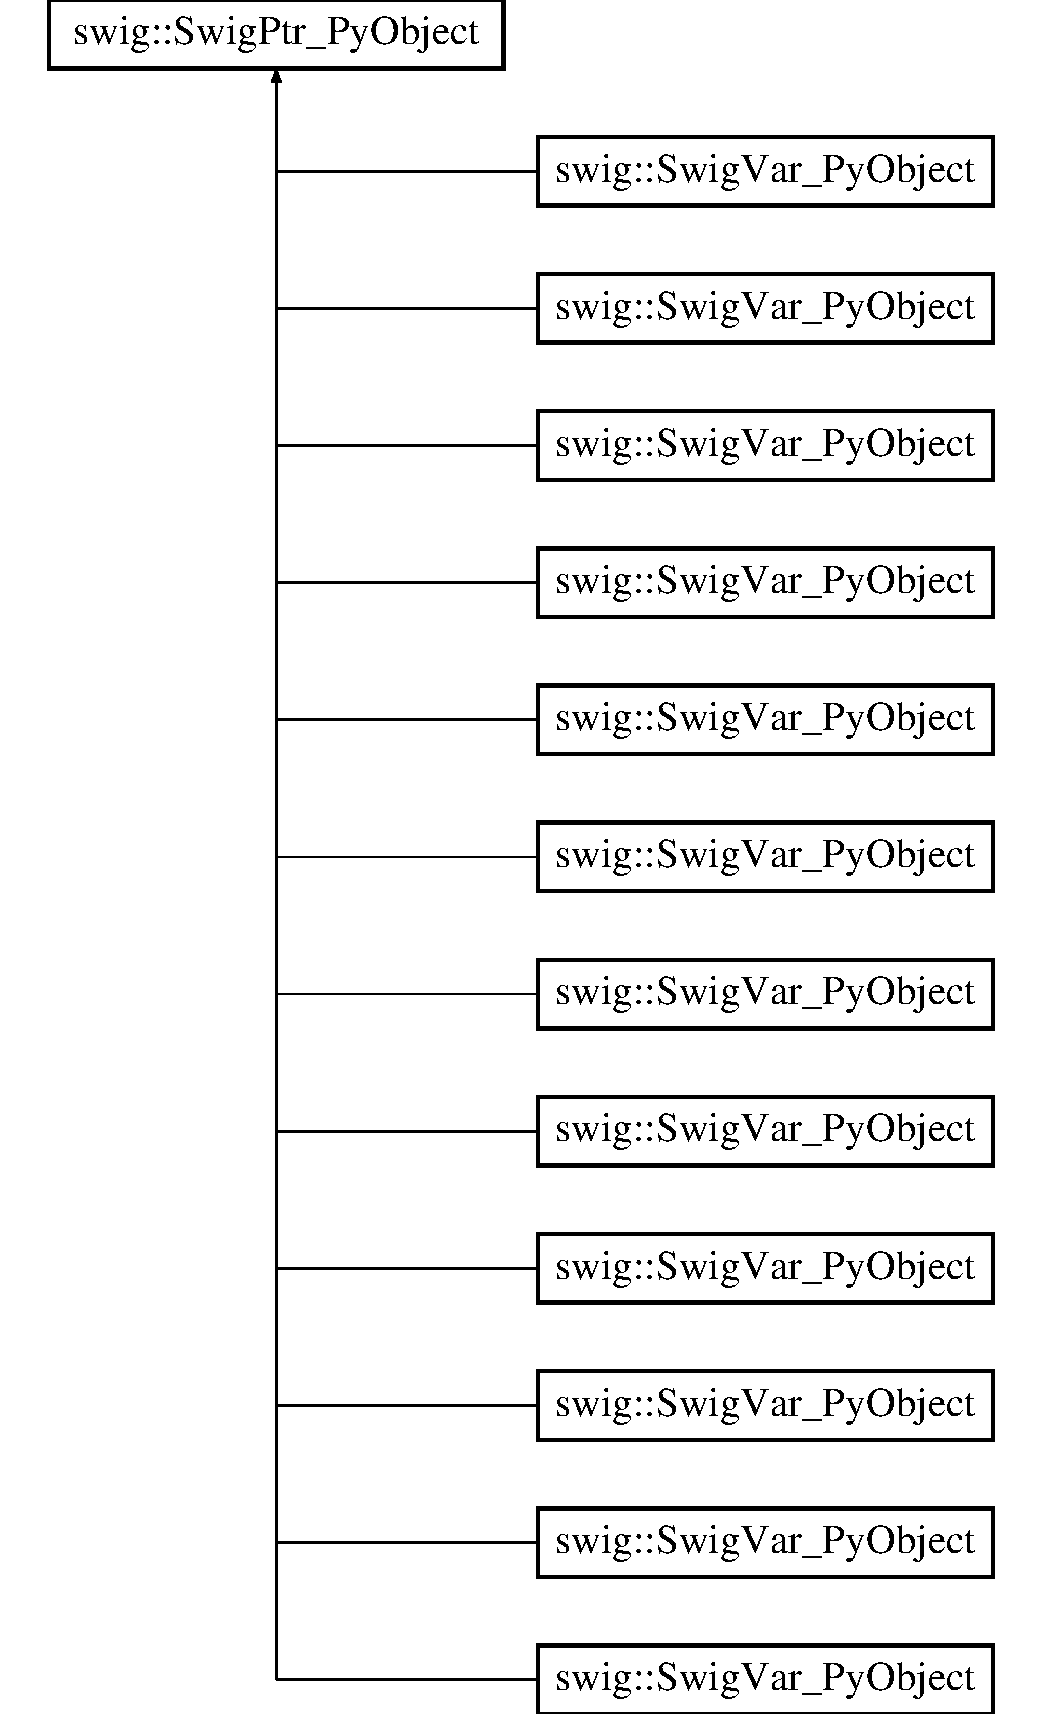
\includegraphics[height=12cm]{d2/d50/classswig_1_1SwigPtr__PyObject}
\end{center}
\end{figure}
\subsection*{Public Member Functions}
\begin{DoxyCompactItemize}
\item 
\hypertarget{classswig_1_1SwigPtr__PyObject_a4282f20207f8cd22c9b079203c832a04}{
{\bfseries SwigPtr\_\-PyObject} (const \hyperlink{classswig_1_1SwigPtr__PyObject}{SwigPtr\_\-PyObject} \&item)}
\label{d2/d50/classswig_1_1SwigPtr__PyObject_a4282f20207f8cd22c9b079203c832a04}

\item 
\hypertarget{classswig_1_1SwigPtr__PyObject_a4503d58d577d209f5e1fa67026852505}{
{\bfseries SwigPtr\_\-PyObject} (PyObject $\ast$obj, bool initial\_\-ref=true)}
\label{d2/d50/classswig_1_1SwigPtr__PyObject_a4503d58d577d209f5e1fa67026852505}

\item 
\hypertarget{classswig_1_1SwigPtr__PyObject_a86d8657d6b4a27c8e9e6942bc1ba572c}{
\hyperlink{classswig_1_1SwigPtr__PyObject}{SwigPtr\_\-PyObject} \& {\bfseries operator=} (const \hyperlink{classswig_1_1SwigPtr__PyObject}{SwigPtr\_\-PyObject} \&item)}
\label{d2/d50/classswig_1_1SwigPtr__PyObject_a86d8657d6b4a27c8e9e6942bc1ba572c}

\item 
\hypertarget{classswig_1_1SwigPtr__PyObject_aa2f1cdba0651c7a52482d225faef0574}{
{\bfseries operator PyObject $\ast$} () const }
\label{d2/d50/classswig_1_1SwigPtr__PyObject_aa2f1cdba0651c7a52482d225faef0574}

\item 
\hypertarget{classswig_1_1SwigPtr__PyObject_a97a20cad6a2b0916f39c45555fb559f0}{
PyObject $\ast$ {\bfseries operator-\/$>$} () const }
\label{d2/d50/classswig_1_1SwigPtr__PyObject_a97a20cad6a2b0916f39c45555fb559f0}

\item 
\hypertarget{classswig_1_1SwigPtr__PyObject_a4282f20207f8cd22c9b079203c832a04}{
{\bfseries SwigPtr\_\-PyObject} (const \hyperlink{classswig_1_1SwigPtr__PyObject}{SwigPtr\_\-PyObject} \&item)}
\label{d2/d50/classswig_1_1SwigPtr__PyObject_a4282f20207f8cd22c9b079203c832a04}

\item 
\hypertarget{classswig_1_1SwigPtr__PyObject_a4503d58d577d209f5e1fa67026852505}{
{\bfseries SwigPtr\_\-PyObject} (PyObject $\ast$obj, bool initial\_\-ref=true)}
\label{d2/d50/classswig_1_1SwigPtr__PyObject_a4503d58d577d209f5e1fa67026852505}

\item 
\hypertarget{classswig_1_1SwigPtr__PyObject_a86d8657d6b4a27c8e9e6942bc1ba572c}{
\hyperlink{classswig_1_1SwigPtr__PyObject}{SwigPtr\_\-PyObject} \& {\bfseries operator=} (const \hyperlink{classswig_1_1SwigPtr__PyObject}{SwigPtr\_\-PyObject} \&item)}
\label{d2/d50/classswig_1_1SwigPtr__PyObject_a86d8657d6b4a27c8e9e6942bc1ba572c}

\item 
\hypertarget{classswig_1_1SwigPtr__PyObject_aa2f1cdba0651c7a52482d225faef0574}{
{\bfseries operator PyObject $\ast$} () const }
\label{d2/d50/classswig_1_1SwigPtr__PyObject_aa2f1cdba0651c7a52482d225faef0574}

\item 
\hypertarget{classswig_1_1SwigPtr__PyObject_a97a20cad6a2b0916f39c45555fb559f0}{
PyObject $\ast$ {\bfseries operator-\/$>$} () const }
\label{d2/d50/classswig_1_1SwigPtr__PyObject_a97a20cad6a2b0916f39c45555fb559f0}

\item 
\hypertarget{classswig_1_1SwigPtr__PyObject_a4282f20207f8cd22c9b079203c832a04}{
{\bfseries SwigPtr\_\-PyObject} (const \hyperlink{classswig_1_1SwigPtr__PyObject}{SwigPtr\_\-PyObject} \&item)}
\label{d2/d50/classswig_1_1SwigPtr__PyObject_a4282f20207f8cd22c9b079203c832a04}

\item 
\hypertarget{classswig_1_1SwigPtr__PyObject_a4503d58d577d209f5e1fa67026852505}{
{\bfseries SwigPtr\_\-PyObject} (PyObject $\ast$obj, bool initial\_\-ref=true)}
\label{d2/d50/classswig_1_1SwigPtr__PyObject_a4503d58d577d209f5e1fa67026852505}

\item 
\hypertarget{classswig_1_1SwigPtr__PyObject_a86d8657d6b4a27c8e9e6942bc1ba572c}{
\hyperlink{classswig_1_1SwigPtr__PyObject}{SwigPtr\_\-PyObject} \& {\bfseries operator=} (const \hyperlink{classswig_1_1SwigPtr__PyObject}{SwigPtr\_\-PyObject} \&item)}
\label{d2/d50/classswig_1_1SwigPtr__PyObject_a86d8657d6b4a27c8e9e6942bc1ba572c}

\item 
\hypertarget{classswig_1_1SwigPtr__PyObject_aa2f1cdba0651c7a52482d225faef0574}{
{\bfseries operator PyObject $\ast$} () const }
\label{d2/d50/classswig_1_1SwigPtr__PyObject_aa2f1cdba0651c7a52482d225faef0574}

\item 
\hypertarget{classswig_1_1SwigPtr__PyObject_a97a20cad6a2b0916f39c45555fb559f0}{
PyObject $\ast$ {\bfseries operator-\/$>$} () const }
\label{d2/d50/classswig_1_1SwigPtr__PyObject_a97a20cad6a2b0916f39c45555fb559f0}

\item 
\hypertarget{classswig_1_1SwigPtr__PyObject_a4282f20207f8cd22c9b079203c832a04}{
{\bfseries SwigPtr\_\-PyObject} (const \hyperlink{classswig_1_1SwigPtr__PyObject}{SwigPtr\_\-PyObject} \&item)}
\label{d2/d50/classswig_1_1SwigPtr__PyObject_a4282f20207f8cd22c9b079203c832a04}

\item 
\hypertarget{classswig_1_1SwigPtr__PyObject_a4503d58d577d209f5e1fa67026852505}{
{\bfseries SwigPtr\_\-PyObject} (PyObject $\ast$obj, bool initial\_\-ref=true)}
\label{d2/d50/classswig_1_1SwigPtr__PyObject_a4503d58d577d209f5e1fa67026852505}

\item 
\hypertarget{classswig_1_1SwigPtr__PyObject_a86d8657d6b4a27c8e9e6942bc1ba572c}{
\hyperlink{classswig_1_1SwigPtr__PyObject}{SwigPtr\_\-PyObject} \& {\bfseries operator=} (const \hyperlink{classswig_1_1SwigPtr__PyObject}{SwigPtr\_\-PyObject} \&item)}
\label{d2/d50/classswig_1_1SwigPtr__PyObject_a86d8657d6b4a27c8e9e6942bc1ba572c}

\item 
\hypertarget{classswig_1_1SwigPtr__PyObject_aa2f1cdba0651c7a52482d225faef0574}{
{\bfseries operator PyObject $\ast$} () const }
\label{d2/d50/classswig_1_1SwigPtr__PyObject_aa2f1cdba0651c7a52482d225faef0574}

\item 
\hypertarget{classswig_1_1SwigPtr__PyObject_a97a20cad6a2b0916f39c45555fb559f0}{
PyObject $\ast$ {\bfseries operator-\/$>$} () const }
\label{d2/d50/classswig_1_1SwigPtr__PyObject_a97a20cad6a2b0916f39c45555fb559f0}

\item 
\hypertarget{classswig_1_1SwigPtr__PyObject_a4282f20207f8cd22c9b079203c832a04}{
{\bfseries SwigPtr\_\-PyObject} (const \hyperlink{classswig_1_1SwigPtr__PyObject}{SwigPtr\_\-PyObject} \&item)}
\label{d2/d50/classswig_1_1SwigPtr__PyObject_a4282f20207f8cd22c9b079203c832a04}

\item 
\hypertarget{classswig_1_1SwigPtr__PyObject_a4503d58d577d209f5e1fa67026852505}{
{\bfseries SwigPtr\_\-PyObject} (PyObject $\ast$obj, bool initial\_\-ref=true)}
\label{d2/d50/classswig_1_1SwigPtr__PyObject_a4503d58d577d209f5e1fa67026852505}

\item 
\hypertarget{classswig_1_1SwigPtr__PyObject_a86d8657d6b4a27c8e9e6942bc1ba572c}{
\hyperlink{classswig_1_1SwigPtr__PyObject}{SwigPtr\_\-PyObject} \& {\bfseries operator=} (const \hyperlink{classswig_1_1SwigPtr__PyObject}{SwigPtr\_\-PyObject} \&item)}
\label{d2/d50/classswig_1_1SwigPtr__PyObject_a86d8657d6b4a27c8e9e6942bc1ba572c}

\item 
\hypertarget{classswig_1_1SwigPtr__PyObject_aa2f1cdba0651c7a52482d225faef0574}{
{\bfseries operator PyObject $\ast$} () const }
\label{d2/d50/classswig_1_1SwigPtr__PyObject_aa2f1cdba0651c7a52482d225faef0574}

\item 
\hypertarget{classswig_1_1SwigPtr__PyObject_a97a20cad6a2b0916f39c45555fb559f0}{
PyObject $\ast$ {\bfseries operator-\/$>$} () const }
\label{d2/d50/classswig_1_1SwigPtr__PyObject_a97a20cad6a2b0916f39c45555fb559f0}

\item 
\hypertarget{classswig_1_1SwigPtr__PyObject_a4282f20207f8cd22c9b079203c832a04}{
{\bfseries SwigPtr\_\-PyObject} (const \hyperlink{classswig_1_1SwigPtr__PyObject}{SwigPtr\_\-PyObject} \&item)}
\label{d2/d50/classswig_1_1SwigPtr__PyObject_a4282f20207f8cd22c9b079203c832a04}

\item 
\hypertarget{classswig_1_1SwigPtr__PyObject_a4503d58d577d209f5e1fa67026852505}{
{\bfseries SwigPtr\_\-PyObject} (PyObject $\ast$obj, bool initial\_\-ref=true)}
\label{d2/d50/classswig_1_1SwigPtr__PyObject_a4503d58d577d209f5e1fa67026852505}

\item 
\hypertarget{classswig_1_1SwigPtr__PyObject_a86d8657d6b4a27c8e9e6942bc1ba572c}{
\hyperlink{classswig_1_1SwigPtr__PyObject}{SwigPtr\_\-PyObject} \& {\bfseries operator=} (const \hyperlink{classswig_1_1SwigPtr__PyObject}{SwigPtr\_\-PyObject} \&item)}
\label{d2/d50/classswig_1_1SwigPtr__PyObject_a86d8657d6b4a27c8e9e6942bc1ba572c}

\item 
\hypertarget{classswig_1_1SwigPtr__PyObject_aa2f1cdba0651c7a52482d225faef0574}{
{\bfseries operator PyObject $\ast$} () const }
\label{d2/d50/classswig_1_1SwigPtr__PyObject_aa2f1cdba0651c7a52482d225faef0574}

\item 
\hypertarget{classswig_1_1SwigPtr__PyObject_a97a20cad6a2b0916f39c45555fb559f0}{
PyObject $\ast$ {\bfseries operator-\/$>$} () const }
\label{d2/d50/classswig_1_1SwigPtr__PyObject_a97a20cad6a2b0916f39c45555fb559f0}

\item 
\hypertarget{classswig_1_1SwigPtr__PyObject_a4282f20207f8cd22c9b079203c832a04}{
{\bfseries SwigPtr\_\-PyObject} (const \hyperlink{classswig_1_1SwigPtr__PyObject}{SwigPtr\_\-PyObject} \&item)}
\label{d2/d50/classswig_1_1SwigPtr__PyObject_a4282f20207f8cd22c9b079203c832a04}

\item 
\hypertarget{classswig_1_1SwigPtr__PyObject_a4503d58d577d209f5e1fa67026852505}{
{\bfseries SwigPtr\_\-PyObject} (PyObject $\ast$obj, bool initial\_\-ref=true)}
\label{d2/d50/classswig_1_1SwigPtr__PyObject_a4503d58d577d209f5e1fa67026852505}

\item 
\hypertarget{classswig_1_1SwigPtr__PyObject_a86d8657d6b4a27c8e9e6942bc1ba572c}{
\hyperlink{classswig_1_1SwigPtr__PyObject}{SwigPtr\_\-PyObject} \& {\bfseries operator=} (const \hyperlink{classswig_1_1SwigPtr__PyObject}{SwigPtr\_\-PyObject} \&item)}
\label{d2/d50/classswig_1_1SwigPtr__PyObject_a86d8657d6b4a27c8e9e6942bc1ba572c}

\item 
\hypertarget{classswig_1_1SwigPtr__PyObject_aa2f1cdba0651c7a52482d225faef0574}{
{\bfseries operator PyObject $\ast$} () const }
\label{d2/d50/classswig_1_1SwigPtr__PyObject_aa2f1cdba0651c7a52482d225faef0574}

\item 
\hypertarget{classswig_1_1SwigPtr__PyObject_a97a20cad6a2b0916f39c45555fb559f0}{
PyObject $\ast$ {\bfseries operator-\/$>$} () const }
\label{d2/d50/classswig_1_1SwigPtr__PyObject_a97a20cad6a2b0916f39c45555fb559f0}

\item 
\hypertarget{classswig_1_1SwigPtr__PyObject_a4282f20207f8cd22c9b079203c832a04}{
{\bfseries SwigPtr\_\-PyObject} (const \hyperlink{classswig_1_1SwigPtr__PyObject}{SwigPtr\_\-PyObject} \&item)}
\label{d2/d50/classswig_1_1SwigPtr__PyObject_a4282f20207f8cd22c9b079203c832a04}

\item 
\hypertarget{classswig_1_1SwigPtr__PyObject_a4503d58d577d209f5e1fa67026852505}{
{\bfseries SwigPtr\_\-PyObject} (PyObject $\ast$obj, bool initial\_\-ref=true)}
\label{d2/d50/classswig_1_1SwigPtr__PyObject_a4503d58d577d209f5e1fa67026852505}

\item 
\hypertarget{classswig_1_1SwigPtr__PyObject_a86d8657d6b4a27c8e9e6942bc1ba572c}{
\hyperlink{classswig_1_1SwigPtr__PyObject}{SwigPtr\_\-PyObject} \& {\bfseries operator=} (const \hyperlink{classswig_1_1SwigPtr__PyObject}{SwigPtr\_\-PyObject} \&item)}
\label{d2/d50/classswig_1_1SwigPtr__PyObject_a86d8657d6b4a27c8e9e6942bc1ba572c}

\item 
\hypertarget{classswig_1_1SwigPtr__PyObject_aa2f1cdba0651c7a52482d225faef0574}{
{\bfseries operator PyObject $\ast$} () const }
\label{d2/d50/classswig_1_1SwigPtr__PyObject_aa2f1cdba0651c7a52482d225faef0574}

\item 
\hypertarget{classswig_1_1SwigPtr__PyObject_a97a20cad6a2b0916f39c45555fb559f0}{
PyObject $\ast$ {\bfseries operator-\/$>$} () const }
\label{d2/d50/classswig_1_1SwigPtr__PyObject_a97a20cad6a2b0916f39c45555fb559f0}

\item 
\hypertarget{classswig_1_1SwigPtr__PyObject_a4282f20207f8cd22c9b079203c832a04}{
{\bfseries SwigPtr\_\-PyObject} (const \hyperlink{classswig_1_1SwigPtr__PyObject}{SwigPtr\_\-PyObject} \&item)}
\label{d2/d50/classswig_1_1SwigPtr__PyObject_a4282f20207f8cd22c9b079203c832a04}

\item 
\hypertarget{classswig_1_1SwigPtr__PyObject_a4503d58d577d209f5e1fa67026852505}{
{\bfseries SwigPtr\_\-PyObject} (PyObject $\ast$obj, bool initial\_\-ref=true)}
\label{d2/d50/classswig_1_1SwigPtr__PyObject_a4503d58d577d209f5e1fa67026852505}

\item 
\hypertarget{classswig_1_1SwigPtr__PyObject_a86d8657d6b4a27c8e9e6942bc1ba572c}{
\hyperlink{classswig_1_1SwigPtr__PyObject}{SwigPtr\_\-PyObject} \& {\bfseries operator=} (const \hyperlink{classswig_1_1SwigPtr__PyObject}{SwigPtr\_\-PyObject} \&item)}
\label{d2/d50/classswig_1_1SwigPtr__PyObject_a86d8657d6b4a27c8e9e6942bc1ba572c}

\item 
\hypertarget{classswig_1_1SwigPtr__PyObject_aa2f1cdba0651c7a52482d225faef0574}{
{\bfseries operator PyObject $\ast$} () const }
\label{d2/d50/classswig_1_1SwigPtr__PyObject_aa2f1cdba0651c7a52482d225faef0574}

\item 
\hypertarget{classswig_1_1SwigPtr__PyObject_a97a20cad6a2b0916f39c45555fb559f0}{
PyObject $\ast$ {\bfseries operator-\/$>$} () const }
\label{d2/d50/classswig_1_1SwigPtr__PyObject_a97a20cad6a2b0916f39c45555fb559f0}

\item 
\hypertarget{classswig_1_1SwigPtr__PyObject_a4282f20207f8cd22c9b079203c832a04}{
{\bfseries SwigPtr\_\-PyObject} (const \hyperlink{classswig_1_1SwigPtr__PyObject}{SwigPtr\_\-PyObject} \&item)}
\label{d2/d50/classswig_1_1SwigPtr__PyObject_a4282f20207f8cd22c9b079203c832a04}

\item 
\hypertarget{classswig_1_1SwigPtr__PyObject_a4503d58d577d209f5e1fa67026852505}{
{\bfseries SwigPtr\_\-PyObject} (PyObject $\ast$obj, bool initial\_\-ref=true)}
\label{d2/d50/classswig_1_1SwigPtr__PyObject_a4503d58d577d209f5e1fa67026852505}

\item 
\hypertarget{classswig_1_1SwigPtr__PyObject_a86d8657d6b4a27c8e9e6942bc1ba572c}{
\hyperlink{classswig_1_1SwigPtr__PyObject}{SwigPtr\_\-PyObject} \& {\bfseries operator=} (const \hyperlink{classswig_1_1SwigPtr__PyObject}{SwigPtr\_\-PyObject} \&item)}
\label{d2/d50/classswig_1_1SwigPtr__PyObject_a86d8657d6b4a27c8e9e6942bc1ba572c}

\item 
\hypertarget{classswig_1_1SwigPtr__PyObject_aa2f1cdba0651c7a52482d225faef0574}{
{\bfseries operator PyObject $\ast$} () const }
\label{d2/d50/classswig_1_1SwigPtr__PyObject_aa2f1cdba0651c7a52482d225faef0574}

\item 
\hypertarget{classswig_1_1SwigPtr__PyObject_a97a20cad6a2b0916f39c45555fb559f0}{
PyObject $\ast$ {\bfseries operator-\/$>$} () const }
\label{d2/d50/classswig_1_1SwigPtr__PyObject_a97a20cad6a2b0916f39c45555fb559f0}

\item 
\hypertarget{classswig_1_1SwigPtr__PyObject_a4282f20207f8cd22c9b079203c832a04}{
{\bfseries SwigPtr\_\-PyObject} (const \hyperlink{classswig_1_1SwigPtr__PyObject}{SwigPtr\_\-PyObject} \&item)}
\label{d2/d50/classswig_1_1SwigPtr__PyObject_a4282f20207f8cd22c9b079203c832a04}

\item 
\hypertarget{classswig_1_1SwigPtr__PyObject_a4503d58d577d209f5e1fa67026852505}{
{\bfseries SwigPtr\_\-PyObject} (PyObject $\ast$obj, bool initial\_\-ref=true)}
\label{d2/d50/classswig_1_1SwigPtr__PyObject_a4503d58d577d209f5e1fa67026852505}

\item 
\hypertarget{classswig_1_1SwigPtr__PyObject_a86d8657d6b4a27c8e9e6942bc1ba572c}{
\hyperlink{classswig_1_1SwigPtr__PyObject}{SwigPtr\_\-PyObject} \& {\bfseries operator=} (const \hyperlink{classswig_1_1SwigPtr__PyObject}{SwigPtr\_\-PyObject} \&item)}
\label{d2/d50/classswig_1_1SwigPtr__PyObject_a86d8657d6b4a27c8e9e6942bc1ba572c}

\item 
\hypertarget{classswig_1_1SwigPtr__PyObject_aa2f1cdba0651c7a52482d225faef0574}{
{\bfseries operator PyObject $\ast$} () const }
\label{d2/d50/classswig_1_1SwigPtr__PyObject_aa2f1cdba0651c7a52482d225faef0574}

\item 
\hypertarget{classswig_1_1SwigPtr__PyObject_a97a20cad6a2b0916f39c45555fb559f0}{
PyObject $\ast$ {\bfseries operator-\/$>$} () const }
\label{d2/d50/classswig_1_1SwigPtr__PyObject_a97a20cad6a2b0916f39c45555fb559f0}

\item 
\hypertarget{classswig_1_1SwigPtr__PyObject_a4282f20207f8cd22c9b079203c832a04}{
{\bfseries SwigPtr\_\-PyObject} (const \hyperlink{classswig_1_1SwigPtr__PyObject}{SwigPtr\_\-PyObject} \&item)}
\label{d2/d50/classswig_1_1SwigPtr__PyObject_a4282f20207f8cd22c9b079203c832a04}

\item 
\hypertarget{classswig_1_1SwigPtr__PyObject_a4503d58d577d209f5e1fa67026852505}{
{\bfseries SwigPtr\_\-PyObject} (PyObject $\ast$obj, bool initial\_\-ref=true)}
\label{d2/d50/classswig_1_1SwigPtr__PyObject_a4503d58d577d209f5e1fa67026852505}

\item 
\hypertarget{classswig_1_1SwigPtr__PyObject_a86d8657d6b4a27c8e9e6942bc1ba572c}{
\hyperlink{classswig_1_1SwigPtr__PyObject}{SwigPtr\_\-PyObject} \& {\bfseries operator=} (const \hyperlink{classswig_1_1SwigPtr__PyObject}{SwigPtr\_\-PyObject} \&item)}
\label{d2/d50/classswig_1_1SwigPtr__PyObject_a86d8657d6b4a27c8e9e6942bc1ba572c}

\item 
\hypertarget{classswig_1_1SwigPtr__PyObject_aa2f1cdba0651c7a52482d225faef0574}{
{\bfseries operator PyObject $\ast$} () const }
\label{d2/d50/classswig_1_1SwigPtr__PyObject_aa2f1cdba0651c7a52482d225faef0574}

\item 
\hypertarget{classswig_1_1SwigPtr__PyObject_a97a20cad6a2b0916f39c45555fb559f0}{
PyObject $\ast$ {\bfseries operator-\/$>$} () const }
\label{d2/d50/classswig_1_1SwigPtr__PyObject_a97a20cad6a2b0916f39c45555fb559f0}

\end{DoxyCompactItemize}
\subsection*{Protected Attributes}
\begin{DoxyCompactItemize}
\item 
\hypertarget{classswig_1_1SwigPtr__PyObject_abb14c2948572bd4bf429540f7770831e}{
PyObject $\ast$ {\bfseries \_\-obj}}
\label{d2/d50/classswig_1_1SwigPtr__PyObject_abb14c2948572bd4bf429540f7770831e}

\end{DoxyCompactItemize}


The documentation for this class was generated from the following files:\begin{DoxyCompactItemize}
\item 
src/convolute\_\-wrap.cxx\item 
src/fittogrid\_\-wrap.cxx\item 
src/integrator\_\-wrap.cxx\item 
src/leastnonmono\_\-wrap.cxx\item 
src/lininterp\_\-wrap.cxx\item 
src/matrix3d\_\-wrap.cxx\item 
src/matrix4d\_\-wrap.cxx\item 
src/matrix\_\-wrap.cxx\item 
src/maxslope\_\-wrap.cxx\item 
src/monocheck\_\-wrap.cxx\item 
src/pdf\_\-wrap.cxx\item 
src/sorting\_\-wrap.cxx\end{DoxyCompactItemize}

\hypertarget{structSwigPyClientData}{
\section{SwigPyClientData Struct Reference}
\label{d5/d6b/structSwigPyClientData}\index{SwigPyClientData@{SwigPyClientData}}
}
\subsection*{Public Attributes}
\begin{DoxyCompactItemize}
\item 
\hypertarget{structSwigPyClientData_afe15f48c719784bf245534c4999ea387}{
PyObject $\ast$ {\bfseries klass}}
\label{d5/d6b/structSwigPyClientData_afe15f48c719784bf245534c4999ea387}

\item 
\hypertarget{structSwigPyClientData_aef35885524e7defa5cbcc00714c4a5c1}{
PyObject $\ast$ {\bfseries newraw}}
\label{d5/d6b/structSwigPyClientData_aef35885524e7defa5cbcc00714c4a5c1}

\item 
\hypertarget{structSwigPyClientData_a8080712504b1249851e64d0baa3926bb}{
PyObject $\ast$ {\bfseries newargs}}
\label{d5/d6b/structSwigPyClientData_a8080712504b1249851e64d0baa3926bb}

\item 
\hypertarget{structSwigPyClientData_a1e3e0efca34cf915f74fdd66ecb9a01e}{
PyObject $\ast$ {\bfseries destroy}}
\label{d5/d6b/structSwigPyClientData_a1e3e0efca34cf915f74fdd66ecb9a01e}

\item 
\hypertarget{structSwigPyClientData_a9cb4b9b02743d09dbe216f304e2b7df0}{
int {\bfseries delargs}}
\label{d5/d6b/structSwigPyClientData_a9cb4b9b02743d09dbe216f304e2b7df0}

\item 
\hypertarget{structSwigPyClientData_a5f9ebdbc04a774559a64b926b6ec4070}{
int {\bfseries implicitconv}}
\label{d5/d6b/structSwigPyClientData_a5f9ebdbc04a774559a64b926b6ec4070}

\end{DoxyCompactItemize}


The documentation for this struct was generated from the following files:\begin{DoxyCompactItemize}
\item 
src/convolute\_\-wrap.cxx\item 
src/fittogrid\_\-wrap.cxx\item 
src/integrator\_\-wrap.cxx\item 
src/leastnonmono\_\-wrap.cxx\item 
src/lininterp\_\-wrap.cxx\item 
src/matrix3d\_\-wrap.cxx\item 
src/matrix4d\_\-wrap.cxx\item 
src/matrix\_\-wrap.cxx\item 
src/maxslope\_\-wrap.cxx\item 
src/monocheck\_\-wrap.cxx\item 
src/pdf\_\-wrap.cxx\item 
src/sorting\_\-wrap.cxx\end{DoxyCompactItemize}

\hypertarget{structSwigPyObject}{
\section{SwigPyObject Struct Reference}
\label{d4/d88/structSwigPyObject}\index{SwigPyObject@{SwigPyObject}}
}
\subsection*{Public Attributes}
\begin{DoxyCompactItemize}
\item 
\hypertarget{structSwigPyObject_a96e168de04fa2da0125cf00f26ea6b9c}{
PyObject\_\-HEAD void $\ast$ {\bfseries ptr}}
\label{d4/d88/structSwigPyObject_a96e168de04fa2da0125cf00f26ea6b9c}

\item 
\hypertarget{structSwigPyObject_a77f6f8357ce9c50f7c18c2a4ea72ea62}{
\hyperlink{structswig__type__info}{swig\_\-type\_\-info} $\ast$ {\bfseries ty}}
\label{d4/d88/structSwigPyObject_a77f6f8357ce9c50f7c18c2a4ea72ea62}

\item 
\hypertarget{structSwigPyObject_a83cb6489fb1b171467f06c091ae6f283}{
int {\bfseries own}}
\label{d4/d88/structSwigPyObject_a83cb6489fb1b171467f06c091ae6f283}

\item 
\hypertarget{structSwigPyObject_a6d423675e9561f658562d3d24f4f70d0}{
PyObject $\ast$ {\bfseries next}}
\label{d4/d88/structSwigPyObject_a6d423675e9561f658562d3d24f4f70d0}

\end{DoxyCompactItemize}


The documentation for this struct was generated from the following files:\begin{DoxyCompactItemize}
\item 
src/convolute\_\-wrap.cxx\item 
src/fittogrid\_\-wrap.cxx\item 
src/integrator\_\-wrap.cxx\item 
src/leastnonmono\_\-wrap.cxx\item 
src/lininterp\_\-wrap.cxx\item 
src/matrix3d\_\-wrap.cxx\item 
src/matrix4d\_\-wrap.cxx\item 
src/matrix\_\-wrap.cxx\item 
src/maxslope\_\-wrap.cxx\item 
src/monocheck\_\-wrap.cxx\item 
src/pdf\_\-wrap.cxx\item 
src/sorting\_\-wrap.cxx\end{DoxyCompactItemize}

\hypertarget{structSwigPyPacked}{
\section{SwigPyPacked Struct Reference}
\label{db/d08/structSwigPyPacked}\index{SwigPyPacked@{SwigPyPacked}}
}
\subsection*{Public Attributes}
\begin{DoxyCompactItemize}
\item 
\hypertarget{structSwigPyPacked_a90bf060d4d9b7924acc8bc81525244d4}{
PyObject\_\-HEAD void $\ast$ {\bfseries pack}}
\label{db/d08/structSwigPyPacked_a90bf060d4d9b7924acc8bc81525244d4}

\item 
\hypertarget{structSwigPyPacked_ae179dcfa49ddb42652601334198d4271}{
\hyperlink{structswig__type__info}{swig\_\-type\_\-info} $\ast$ {\bfseries ty}}
\label{db/d08/structSwigPyPacked_ae179dcfa49ddb42652601334198d4271}

\item 
\hypertarget{structSwigPyPacked_aed2bfb8fb3c9f804c386215db63921cb}{
size\_\-t {\bfseries size}}
\label{db/d08/structSwigPyPacked_aed2bfb8fb3c9f804c386215db63921cb}

\end{DoxyCompactItemize}


The documentation for this struct was generated from the following files:\begin{DoxyCompactItemize}
\item 
src/convolute\_\-wrap.cxx\item 
src/fittogrid\_\-wrap.cxx\item 
src/integrator\_\-wrap.cxx\item 
src/leastnonmono\_\-wrap.cxx\item 
src/lininterp\_\-wrap.cxx\item 
src/matrix3d\_\-wrap.cxx\item 
src/matrix4d\_\-wrap.cxx\item 
src/matrix\_\-wrap.cxx\item 
src/maxslope\_\-wrap.cxx\item 
src/monocheck\_\-wrap.cxx\item 
src/pdf\_\-wrap.cxx\item 
src/sorting\_\-wrap.cxx\end{DoxyCompactItemize}

\hypertarget{structswig_1_1SwigVar__PyObject}{
\section{swig::SwigVar\_\-PyObject Struct Reference}
\label{de/d74/structswig_1_1SwigVar__PyObject}\index{swig::SwigVar\_\-PyObject@{swig::SwigVar\_\-PyObject}}
}
Inheritance diagram for swig::SwigVar\_\-PyObject::\begin{figure}[H]
\begin{center}
\leavevmode
\includegraphics[height=12cm]{de/d74/structswig_1_1SwigVar__PyObject}
\end{center}
\end{figure}
\subsection*{Public Member Functions}
\begin{DoxyCompactItemize}
\item 
\hypertarget{structswig_1_1SwigVar__PyObject_a2b61f843215bceaff8ec2ea6e92d46c2}{
{\bfseries SwigVar\_\-PyObject} (PyObject $\ast$obj=0)}
\label{de/d74/structswig_1_1SwigVar__PyObject_a2b61f843215bceaff8ec2ea6e92d46c2}

\item 
\hypertarget{structswig_1_1SwigVar__PyObject_a7e6053b64cf6e787b99a67b09cdc6d89}{
\hyperlink{structswig_1_1SwigVar__PyObject}{SwigVar\_\-PyObject} \& {\bfseries operator=} (PyObject $\ast$obj)}
\label{de/d74/structswig_1_1SwigVar__PyObject_a7e6053b64cf6e787b99a67b09cdc6d89}

\item 
\hypertarget{structswig_1_1SwigVar__PyObject_a2b61f843215bceaff8ec2ea6e92d46c2}{
{\bfseries SwigVar\_\-PyObject} (PyObject $\ast$obj=0)}
\label{de/d74/structswig_1_1SwigVar__PyObject_a2b61f843215bceaff8ec2ea6e92d46c2}

\item 
\hypertarget{structswig_1_1SwigVar__PyObject_a7e6053b64cf6e787b99a67b09cdc6d89}{
\hyperlink{structswig_1_1SwigVar__PyObject}{SwigVar\_\-PyObject} \& {\bfseries operator=} (PyObject $\ast$obj)}
\label{de/d74/structswig_1_1SwigVar__PyObject_a7e6053b64cf6e787b99a67b09cdc6d89}

\item 
\hypertarget{structswig_1_1SwigVar__PyObject_a2b61f843215bceaff8ec2ea6e92d46c2}{
{\bfseries SwigVar\_\-PyObject} (PyObject $\ast$obj=0)}
\label{de/d74/structswig_1_1SwigVar__PyObject_a2b61f843215bceaff8ec2ea6e92d46c2}

\item 
\hypertarget{structswig_1_1SwigVar__PyObject_a7e6053b64cf6e787b99a67b09cdc6d89}{
\hyperlink{structswig_1_1SwigVar__PyObject}{SwigVar\_\-PyObject} \& {\bfseries operator=} (PyObject $\ast$obj)}
\label{de/d74/structswig_1_1SwigVar__PyObject_a7e6053b64cf6e787b99a67b09cdc6d89}

\item 
\hypertarget{structswig_1_1SwigVar__PyObject_a2b61f843215bceaff8ec2ea6e92d46c2}{
{\bfseries SwigVar\_\-PyObject} (PyObject $\ast$obj=0)}
\label{de/d74/structswig_1_1SwigVar__PyObject_a2b61f843215bceaff8ec2ea6e92d46c2}

\item 
\hypertarget{structswig_1_1SwigVar__PyObject_a7e6053b64cf6e787b99a67b09cdc6d89}{
\hyperlink{structswig_1_1SwigVar__PyObject}{SwigVar\_\-PyObject} \& {\bfseries operator=} (PyObject $\ast$obj)}
\label{de/d74/structswig_1_1SwigVar__PyObject_a7e6053b64cf6e787b99a67b09cdc6d89}

\item 
\hypertarget{structswig_1_1SwigVar__PyObject_a2b61f843215bceaff8ec2ea6e92d46c2}{
{\bfseries SwigVar\_\-PyObject} (PyObject $\ast$obj=0)}
\label{de/d74/structswig_1_1SwigVar__PyObject_a2b61f843215bceaff8ec2ea6e92d46c2}

\item 
\hypertarget{structswig_1_1SwigVar__PyObject_a7e6053b64cf6e787b99a67b09cdc6d89}{
\hyperlink{structswig_1_1SwigVar__PyObject}{SwigVar\_\-PyObject} \& {\bfseries operator=} (PyObject $\ast$obj)}
\label{de/d74/structswig_1_1SwigVar__PyObject_a7e6053b64cf6e787b99a67b09cdc6d89}

\item 
\hypertarget{structswig_1_1SwigVar__PyObject_a2b61f843215bceaff8ec2ea6e92d46c2}{
{\bfseries SwigVar\_\-PyObject} (PyObject $\ast$obj=0)}
\label{de/d74/structswig_1_1SwigVar__PyObject_a2b61f843215bceaff8ec2ea6e92d46c2}

\item 
\hypertarget{structswig_1_1SwigVar__PyObject_a7e6053b64cf6e787b99a67b09cdc6d89}{
\hyperlink{structswig_1_1SwigVar__PyObject}{SwigVar\_\-PyObject} \& {\bfseries operator=} (PyObject $\ast$obj)}
\label{de/d74/structswig_1_1SwigVar__PyObject_a7e6053b64cf6e787b99a67b09cdc6d89}

\item 
\hypertarget{structswig_1_1SwigVar__PyObject_a2b61f843215bceaff8ec2ea6e92d46c2}{
{\bfseries SwigVar\_\-PyObject} (PyObject $\ast$obj=0)}
\label{de/d74/structswig_1_1SwigVar__PyObject_a2b61f843215bceaff8ec2ea6e92d46c2}

\item 
\hypertarget{structswig_1_1SwigVar__PyObject_a7e6053b64cf6e787b99a67b09cdc6d89}{
\hyperlink{structswig_1_1SwigVar__PyObject}{SwigVar\_\-PyObject} \& {\bfseries operator=} (PyObject $\ast$obj)}
\label{de/d74/structswig_1_1SwigVar__PyObject_a7e6053b64cf6e787b99a67b09cdc6d89}

\item 
\hypertarget{structswig_1_1SwigVar__PyObject_a2b61f843215bceaff8ec2ea6e92d46c2}{
{\bfseries SwigVar\_\-PyObject} (PyObject $\ast$obj=0)}
\label{de/d74/structswig_1_1SwigVar__PyObject_a2b61f843215bceaff8ec2ea6e92d46c2}

\item 
\hypertarget{structswig_1_1SwigVar__PyObject_a7e6053b64cf6e787b99a67b09cdc6d89}{
\hyperlink{structswig_1_1SwigVar__PyObject}{SwigVar\_\-PyObject} \& {\bfseries operator=} (PyObject $\ast$obj)}
\label{de/d74/structswig_1_1SwigVar__PyObject_a7e6053b64cf6e787b99a67b09cdc6d89}

\item 
\hypertarget{structswig_1_1SwigVar__PyObject_a2b61f843215bceaff8ec2ea6e92d46c2}{
{\bfseries SwigVar\_\-PyObject} (PyObject $\ast$obj=0)}
\label{de/d74/structswig_1_1SwigVar__PyObject_a2b61f843215bceaff8ec2ea6e92d46c2}

\item 
\hypertarget{structswig_1_1SwigVar__PyObject_a7e6053b64cf6e787b99a67b09cdc6d89}{
\hyperlink{structswig_1_1SwigVar__PyObject}{SwigVar\_\-PyObject} \& {\bfseries operator=} (PyObject $\ast$obj)}
\label{de/d74/structswig_1_1SwigVar__PyObject_a7e6053b64cf6e787b99a67b09cdc6d89}

\item 
\hypertarget{structswig_1_1SwigVar__PyObject_a2b61f843215bceaff8ec2ea6e92d46c2}{
{\bfseries SwigVar\_\-PyObject} (PyObject $\ast$obj=0)}
\label{de/d74/structswig_1_1SwigVar__PyObject_a2b61f843215bceaff8ec2ea6e92d46c2}

\item 
\hypertarget{structswig_1_1SwigVar__PyObject_a7e6053b64cf6e787b99a67b09cdc6d89}{
\hyperlink{structswig_1_1SwigVar__PyObject}{SwigVar\_\-PyObject} \& {\bfseries operator=} (PyObject $\ast$obj)}
\label{de/d74/structswig_1_1SwigVar__PyObject_a7e6053b64cf6e787b99a67b09cdc6d89}

\item 
\hypertarget{structswig_1_1SwigVar__PyObject_a2b61f843215bceaff8ec2ea6e92d46c2}{
{\bfseries SwigVar\_\-PyObject} (PyObject $\ast$obj=0)}
\label{de/d74/structswig_1_1SwigVar__PyObject_a2b61f843215bceaff8ec2ea6e92d46c2}

\item 
\hypertarget{structswig_1_1SwigVar__PyObject_a7e6053b64cf6e787b99a67b09cdc6d89}{
\hyperlink{structswig_1_1SwigVar__PyObject}{SwigVar\_\-PyObject} \& {\bfseries operator=} (PyObject $\ast$obj)}
\label{de/d74/structswig_1_1SwigVar__PyObject_a7e6053b64cf6e787b99a67b09cdc6d89}

\item 
\hypertarget{structswig_1_1SwigVar__PyObject_a2b61f843215bceaff8ec2ea6e92d46c2}{
{\bfseries SwigVar\_\-PyObject} (PyObject $\ast$obj=0)}
\label{de/d74/structswig_1_1SwigVar__PyObject_a2b61f843215bceaff8ec2ea6e92d46c2}

\item 
\hypertarget{structswig_1_1SwigVar__PyObject_a7e6053b64cf6e787b99a67b09cdc6d89}{
\hyperlink{structswig_1_1SwigVar__PyObject}{SwigVar\_\-PyObject} \& {\bfseries operator=} (PyObject $\ast$obj)}
\label{de/d74/structswig_1_1SwigVar__PyObject_a7e6053b64cf6e787b99a67b09cdc6d89}

\end{DoxyCompactItemize}


The documentation for this struct was generated from the following files:\begin{DoxyCompactItemize}
\item 
src/convolute\_\-wrap.cxx\item 
src/fittogrid\_\-wrap.cxx\item 
src/integrator\_\-wrap.cxx\item 
src/leastnonmono\_\-wrap.cxx\item 
src/lininterp\_\-wrap.cxx\item 
src/matrix3d\_\-wrap.cxx\item 
src/matrix4d\_\-wrap.cxx\item 
src/matrix\_\-wrap.cxx\item 
src/maxslope\_\-wrap.cxx\item 
src/monocheck\_\-wrap.cxx\item 
src/pdf\_\-wrap.cxx\item 
src/sorting\_\-wrap.cxx\end{DoxyCompactItemize}

\hypertarget{classTrapz}{
\section{Trapz Class Reference}
\label{d8/da8/classTrapz}\index{Trapz@{Trapz}}
}


Calculates integral using the trapezoidal method.  


{\ttfamily \#include $<$trapz.h$>$}Inheritance diagram for Trapz::\begin{figure}[H]
\begin{center}
\leavevmode
\includegraphics[height=2cm]{d8/da8/classTrapz}
\end{center}
\end{figure}
\subsection*{Public Member Functions}
\begin{DoxyCompactItemize}
\item 
\hypertarget{classTrapz_a464cc7e5b33620d799cb89f69f70f1b4}{
\hyperlink{classTrapz_a464cc7e5b33620d799cb89f69f70f1b4}{Trapz} ()}
\label{d8/da8/classTrapz_a464cc7e5b33620d799cb89f69f70f1b4}

\begin{DoxyCompactList}\small\item\em Constructor. \item\end{DoxyCompactList}\item 
\hypertarget{classTrapz_adff2586590ecb48620b749a0966f32a7}{
\hyperlink{classTrapz_adff2586590ecb48620b749a0966f32a7}{$\sim$Trapz} ()}
\label{d8/da8/classTrapz_adff2586590ecb48620b749a0966f32a7}

\begin{DoxyCompactList}\small\item\em Destructor. \item\end{DoxyCompactList}\item 
double \hyperlink{classTrapz_a8aee327ed631f75ef3dea7e458f71cca}{integrate} (const double $\ast$integrand, const double $\ast$Z, const int ZPoints)
\begin{DoxyCompactList}\small\item\em Main function that integrates a given data set using Trapezoidal Rule. \item\end{DoxyCompactList}\end{DoxyCompactItemize}


\subsection{Detailed Description}
Calculates integral using the trapezoidal method. \hyperlink{classTrapz}{Trapz} takes in an array (the integrand) and returns the integral of that array using the trapezoidal method. 

\subsection{Member Function Documentation}
\hypertarget{classTrapz_a8aee327ed631f75ef3dea7e458f71cca}{
\index{Trapz@{Trapz}!integrate@{integrate}}
\index{integrate@{integrate}!Trapz@{Trapz}}
\subsubsection[{integrate}]{\setlength{\rightskip}{0pt plus 5cm}double Trapz::integrate (const double $\ast$ {\em integrand}, \/  const double $\ast$ {\em Z}, \/  const int {\em ZPoints})\hspace{0.3cm}{\ttfamily  \mbox{[}virtual\mbox{]}}}}
\label{d8/da8/classTrapz_a8aee327ed631f75ef3dea7e458f71cca}


Main function that integrates a given data set using Trapezoidal Rule. Trapezoidal rule is applied to integrate a given integrand over a given double array, Z.

\begin{DoxyVerb}
  INPUTS:

  const double *integrand          array that contains function values to be integrated

  const double *Z                  array that contains the mixture fraction values which the integrand will be integrated over

  const int ZPoints                number of values, size of the integrand and Z containers

  
  OUTPUT:

  double                           result of the integration
 
  \end{DoxyVerb}
 

Implements \hyperlink{classIntegrator_a89fbef2f7923ce4e2c979b2ff1d1f4ac}{Integrator}.

The documentation for this class was generated from the following files:\begin{DoxyCompactItemize}
\item 
src/trapz.h\item 
src/trapz.cc\end{DoxyCompactItemize}

\hypertarget{classintegrator_1_1Trapz}{
\section{integrator::Trapz Class Reference}
\label{db/dc8/classintegrator_1_1Trapz}\index{integrator::Trapz@{integrator::Trapz}}
}
Inheritance diagram for integrator::Trapz::\begin{figure}[H]
\begin{center}
\leavevmode
\includegraphics[height=3cm]{db/dc8/classintegrator_1_1Trapz}
\end{center}
\end{figure}
\subsection*{Public Member Functions}
\begin{DoxyCompactItemize}
\item 
\hypertarget{classintegrator_1_1Trapz_a20001d1505a9f9f5d6412e707c99a28c}{
def {\bfseries \_\-\_\-init\_\-\_\-}}
\label{db/dc8/classintegrator_1_1Trapz_a20001d1505a9f9f5d6412e707c99a28c}

\item 
\hypertarget{classintegrator_1_1Trapz_af8fade81b71ebd43ea4d8c93b7dbc490}{
def {\bfseries integrate}}
\label{db/dc8/classintegrator_1_1Trapz_af8fade81b71ebd43ea4d8c93b7dbc490}

\end{DoxyCompactItemize}
\subsection*{Public Attributes}
\begin{DoxyCompactItemize}
\item 
\hypertarget{classintegrator_1_1Trapz_a591c3fae4b831990a14bf6ac6203d599}{
{\bfseries this}}
\label{db/dc8/classintegrator_1_1Trapz_a591c3fae4b831990a14bf6ac6203d599}

\end{DoxyCompactItemize}


The documentation for this class was generated from the following file:\begin{DoxyCompactItemize}
\item 
src/integrator.py\end{DoxyCompactItemize}

\printindex
\end{document}
